\documentclass[10pt, a4paper]{article}
\usepackage[left=2.00cm, right=2.00cm, top=2.00cm, bottom=2.00cm]{geometry}
\usepackage{supertabular}
\usepackage{graphicx}
\usepackage{float}
\usepackage[fontset=windows]{ctex}
\usepackage{amsmath,amssymb,amsthm}
\usepackage{unicode-math}
\usepackage{verbatim}
\usepackage{multirow}
\usepackage{pifont}
\usepackage{caption}
\usepackage{diagbox}
\usepackage{listings}
\usepackage{algorithm}  
\usepackage{algpseudocode}
\usepackage{booktabs}   
\usepackage{underscore}
\usepackage{xcolor}
\lstset{
  %行号
  numbers=left,
  %背景框
  frame=single,
  rulecolor=\color[rgb]{0.8,0.8,0.8},         % 设置代码框颜色
  breaklines,                                 % 自动将长的代码行换行排版
  extendedchars=false,                        % 解决代码跨页时,章节标题,页眉等汉字不显示的问题
  %背景色
  %backgroundcolor=\color[rgb]{1,1,0.76},
  backgroundcolor=\color[RGB]{245,245,244},
  %样式
  keywordstyle=\bf\color{blue},
  identifierstyle=\bf,
  numberstyle=\color[RGB]{0,192,192},
  commentstyle=\it\color[RGB]{0,96,96},
  stringstyle=\rmfamily\slshape\color[RGB]{128,0,0},
  %显示空格
  showstringspaces=false
}

\setcounter{secnumdepth}{4}
\setcounter{tocdepth}{4}
\newcommand{\whiteding}[1]{\ding{\numexpr171+#1\relax}}
\newcommand\vbf{\symbfit}
\newtheorem{definition}{\hspace{2em}定义}
\newtheorem{theorem}{\hspace{2em}定理}
\renewcommand{\algorithmicrequire}{\textbf{Input:}}  % Use Input in the format of Algorithm  
\renewcommand{\algorithmicensure}{\textbf{Output:}} % Use Output in the format of Algorithm  

\title{\heiti 大作业4\phantom{   }FPU模型}
\author{ 张钰坤 \\  2000011314 \\(C语言实现)}
\date{2022年5月1日}

\begin{document}
    \maketitle
    \tableofcontents
    \newpage

    \section{题目解答}

    \subsection{第一问}

    下面解析地证明系统本征模式具有题目所给形式。
    
    对于没有高次项的情形,体系哈密顿量具有形式

    \begin{align}
        H&=\frac{1}{2}\sum_{j=1}^np_j^2+\frac{1}{2}\sum_{j=0}^n(q_j-q_{j+1})^2\\
        &=\frac{1}{2}\vbf{p}^\top \vbf{p}+\frac{1}{2}\vbf{q}^\top \vbf{Kq}
    \end{align}

    其中,

    \begin{align*}
        \vbf{K}=
        \begin{pmatrix}
            2&-1&0&\cdots&0&0\\
            -1&2&-1&\cdots&0&0\\
            0&-1&2&\cdots&0&0\\
            \vdots&\vdots&\vdots&\ddots &\vdots&\vdots\\
            0&0&0&\cdots&2&-1\\
            0&0&0&\cdots&-1&2
        \end{pmatrix}
    \end{align*}

    欲求系统本征模式,需要将K对角化。

    下面将会证明:

    \begin{align}
        \vbf{K}&=\vbf{P^\top D P}\\
        P_{kj}&=\sqrt{\frac{2}{n+1}}\sin{\frac{\pi k j}{n+1}}, \vbf{D}=diag\{\omega_1^2,\cdots,\omega_n^2\},\omega_k=2\sin\frac{\pi k}{2(n+1)}
    \end{align}

    注意到可以将K写为

    \[\vbf{K}=2\vbf{I}-\vbf{T}\]

    其中,

    \[T=
    \begin{pmatrix}
        0&1&0&\cdots&0&0\\
        1&0&1&\cdots&0&0\\
        0&1&0&\cdots&0&0\\
        \vdots&\vdots&\vdots&\ddots &\vdots&\vdots\\
        0&0&0&\cdots&0&1\\
        0&0&0&\cdots&1&0
    \end{pmatrix}\]

    可以知道,K和T的本征向量相同,K的本征值$\mu$和T的本征值$\lambda$满足关系$\mu=2-\lambda$。因此,我们只要求得T的本征值、本征向量,就可以得到K的本征值、本征向量。

    设T的本征值$\lambda=2c$(实对称矩阵T一定有$c\in \mathbb{R}$),本征向量$\vbf{v}=(v_1,v_2,\cdots,v_n)^\top$。我们稍后将会看到,把$\lambda$设为2c只是为了数学上的方便。

    于是有,

    \begin{align*}
        0=(\vbf{T}-\lambda\vbf{I})\vbf{v}&=
        \begin{pmatrix}
            -2c&1&0&\cdots&0&0\\
            1&-2c&1&\cdots&0&0\\
            0&1&-2c&\cdots&0&0\\
            \vdots&\vdots&\vdots&\ddots &\vdots&\vdots\\
            0&0&0&\cdots&-2c&1\\
            0&0&0&\cdots&1&-2c
        \end{pmatrix}
        \begin{pmatrix}
            v_1\\
            v_2\\
            v_3\\
            \vdots\\
            v_{n-1}\\
            v_n
        \end{pmatrix}\\
        &\\
        &=
        \begin{pmatrix}
            -2cv_1+v_2\\
            v_1-2cv_2+v_3\\
            \vdots\\
            v_{j-1}-2cv_j+v_{j+1}\\
            \vdots\\
            v_{n-2}-2cv_{n-1}+v_n\\
            v_{n-1}-2cv_n
        \end{pmatrix}
    \end{align*}

    除了第一个和最后一个方程,其他都有$ v_{j-1}-2cv_j+v_{j+1}=0$的形式,为了使第一个和最后一个方程也具有这样的形式,我们引入$v_0=v_{n+1}=0$,这样所有$v_i$都满足如下关系

    \begin{equation}
        v_{j-1}-2cv_j+v_{j+1}=0,j=1,2,\cdots,n
    \end{equation}\label{eq:第一问递推关系}

    如果我们把$\vbf{v}=(v_1,v_2,\cdots,v_n)^\top$中每个元素看成一个数列$\{v_j\}$,那么上式给出了这个数列的二阶递推关系。根据二阶常系数递推数列的一般解法,我们设$v_j=r^j$,方程\ref{eq:第一问递推关系}给出$1-2cr+r^2=0$,得到两个根。
    \[r_\pm=c\pm\sqrt{c^2-1}\]

    我们将对$c^2=1$和$c^2\neq 1$分别讨论。

    当$c^2=1$时,r=c并且方程\ref{eq:第一问递推关系}的通解为
    \[v_j=(A+Bj)c^j\]
    根据边界条件$v_0=v_{n+1}=0$,得到$A=0,(A+B(n+1))c^{n+1}=0$,于是$A=B=0$。由于特征向量一定非零,所以$c^2$一定不为1。

    当$c^2\neq1$时,设$r:=r_+=c+\sqrt{c^2-1}$,于是$r_-=c-\sqrt{c^2-1}=1/r$,这样,方程\ref{eq:第一问递推关系}的解就可以写为
    \[v_j=Ar_+^j+Br_-^j=Ar^j+Br^{-j},\text{   }j=0,\cdots,n+1\]

    应用边界条件$v_0=0$得到$A+B=0$,我们得到
    \[v_j=A(r^j-r^{-j}),\text{   }j=0,\cdots,n+1\]

    由于特征向量非零,需要$A\neq0$,再根据边界条件$v_{n+1}=0$我们得到
    \[r^{n+1}-r^{-(n+1)}=0\Longrightarrow r^{2(n+1)}=1\]

    设$r=e^{i\theta}$,则$c=\cos \theta$且$1=e^{2i(n+1)\theta}$。于是$\theta=k\pi/(n+1),1\le k\le n$(这里排除掉k=0和k=n+1是因为$c^2\neq1$)。接着,取$A=1/(2i)$,我们就得到了T的特征向量

    \[\vbf{v}_k=(\sin\frac{\pi k}{n+1},\sin\frac{2\pi k}{n+1},\cdots,\sin\frac{n\pi k}{n+1})^\top\]

    由于

    \begin{align*}
        &\forall k=1,2,\dots,n\\
        &\sin^2\frac{\pi k}{n+1}+\sin^2\frac{2\pi k}{n+1}+\cdots+\sin^2\frac{n\pi k}{n+1}\\
        =&\frac{1-\cos\frac{2\pi k}{n+1}}{2}+\frac{1-\cos\frac{4\pi k}{n+1}}{2}+\cdots+\frac{1-\cos\frac{2n\pi k}{n+1}}{2}\\
        =&\frac{n}{2}-\frac{1}{2}(\cos\frac{2\pi k}{n+1}+\cos\frac{4\pi k}{n+1}+\dots+\cos\frac{2n\pi k}{n+1})\\
        =&\frac{n}{2}-\frac{1}{2}(\Re(e^{i\frac{2\pi k}{n+1}}+e^{i\frac{4\pi k}{n+1}}+\dots+e^{i\frac{2n\pi k}{n+1}}))\\
        =&\frac{n+1}{2}
    \end{align*}

    所以特征向量需要引入正交化因子$\sqrt{2/(n+1)}$。

    根据上述讨论,我们得到T的特征值是$\lambda=2c=2\cos (k\pi/(n+1))$,特征向量
    
    $\vbf{v}_k=\sqrt{\frac{2}{n+1}}(\sin\frac{\pi k}{n+1},\sin\frac{2\pi k}{n+1},\cdots,\sin\frac{n\pi k}{n+1})^\top$

    再根据K和T的关系,得到K的特征值$\mu=2-\lambda=2-2\cos (k\pi/(n+1))=(2\sin\frac{k\pi}{2(n+1)})^2=\omega_k^2$,特征向量$\vbf{v}_k=\sqrt{\frac{2}{n+1}}(\sin\frac{\pi k}{n+1},\sin\frac{2\pi k}{n+1},\cdots,\sin\frac{n\pi k}{n+1})^\top$

    于是
    \[\vbf{K}=(\vbf{v}_1,\vbf{v}_2,\cdots,\vbf{v}_n)^\top diag\{\omega_1^2,\omega_2^2,\dots,\omega_n^2\}(\vbf{v}_1,\vbf{v}_2,\cdots,\vbf{v}_n)=\vbf{P}^\top\vbf{D}\vbf{P}\]

    其中P是正交矩阵。容易知道$P[i;j]=\sqrt{\frac{2}{n+1}}\sin\frac{\pi i j}{n+1}$,i、j对称,P还是对称矩阵。

    设

    \begin{equation}
        \vbf{Q}=\vbf{Pq}
    \end{equation}\label{eq:真实位形到简正模式的变换}
    
    体系哈密顿量可以改写为

    \begin{align*}
        \vbf{H}&=\frac{1}{2}\vbf{\dot{q} }^\top \vbf{\dot{q} }+\frac{1}{2}\vbf{q}^\top \vbf{Kq}=\frac{1}{2}\vbf{\dot{q} }^\top \vbf{P^\top P\dot{q} }+\frac{1}{2}\vbf{q}^\top \vbf{P^\top D P q}\\
        &=\frac{1}{2}\vbf{\dot{Q} }^\top \vbf{\dot{Q} }+\frac{1}{2}\vbf{Q}^\top \vbf{DQ}\\
        &=\frac{1}{2}\begin{pmatrix}
            Q_1,Q_2,\dots,Q_n
        \end{pmatrix}
        \begin{pmatrix}
            Q_1\\
            Q_2\\
            \vdots\\
            Q_n
        \end{pmatrix}   
        +\frac{1}{2}
        \begin{pmatrix}
            Q_1,Q_2,\dots,Q_n
        \end{pmatrix}
        \begin{pmatrix}
            \omega_1^2&&&\\
            &\omega_2^2&&\\
            &&\ddots&\\
            &&&\omega_n^2
        \end{pmatrix}
        \begin{pmatrix}
            Q_1\\
            Q_2\\
            \vdots\\
            Q_n
        \end{pmatrix}  
    \end{align*}

    于是就得到了体系n个本征模式的能量$E_k=\frac{1}{2}\dot{Q}_k^2+\frac{1}{2}\omega_k^2 Q_k^2$
    其中$Q_k=\sqrt{\frac{2}{n+1}}\sum_{j=1}^n\sin\frac{\pi k j}{n+1}q_j,\omega_k=2\sin\frac{\pi k}{2(n+1)}$

    \subsection{第二问}

    这一问本质上需要解决两个问题:

    \textbf{问题一:}根据各个简正模式的初始位置确定各个质点在真实相空间的初始位置;

    \textbf{问题二:}求解系统随时间的演化,并计算前四个简正模式的能量。

    \subsubsection{思路分析}

    \textbf{问题一:}
    由于质点的真实位形和简正模式位形通过一个正交变换联系(方程\ref{eq:真实位形到简正模式的变换}),给定简正模式位形可以求出真实位形,这只需解一个线性方程组即可。由于P是正交矩阵,是满秩的,于是可以采用列主元的Doolittle分解法求解。

    \textbf{问题二:}
    这是个哈密顿系统,为保证能量守恒,应采用辛算法求解系统随时间的演化。由于蛙跳法是辛的,这里可以采用蛙跳法进行。

    \textbf{具体代码实现见附录"q2.c"。}

    这里展示$E_1,E_2,E_3,E_4$随时间的变化,时间轴单位取$2\pi/\omega_1$。(原始数据见“q2.txt”)

    \begin{figure}[H]
        \centering
        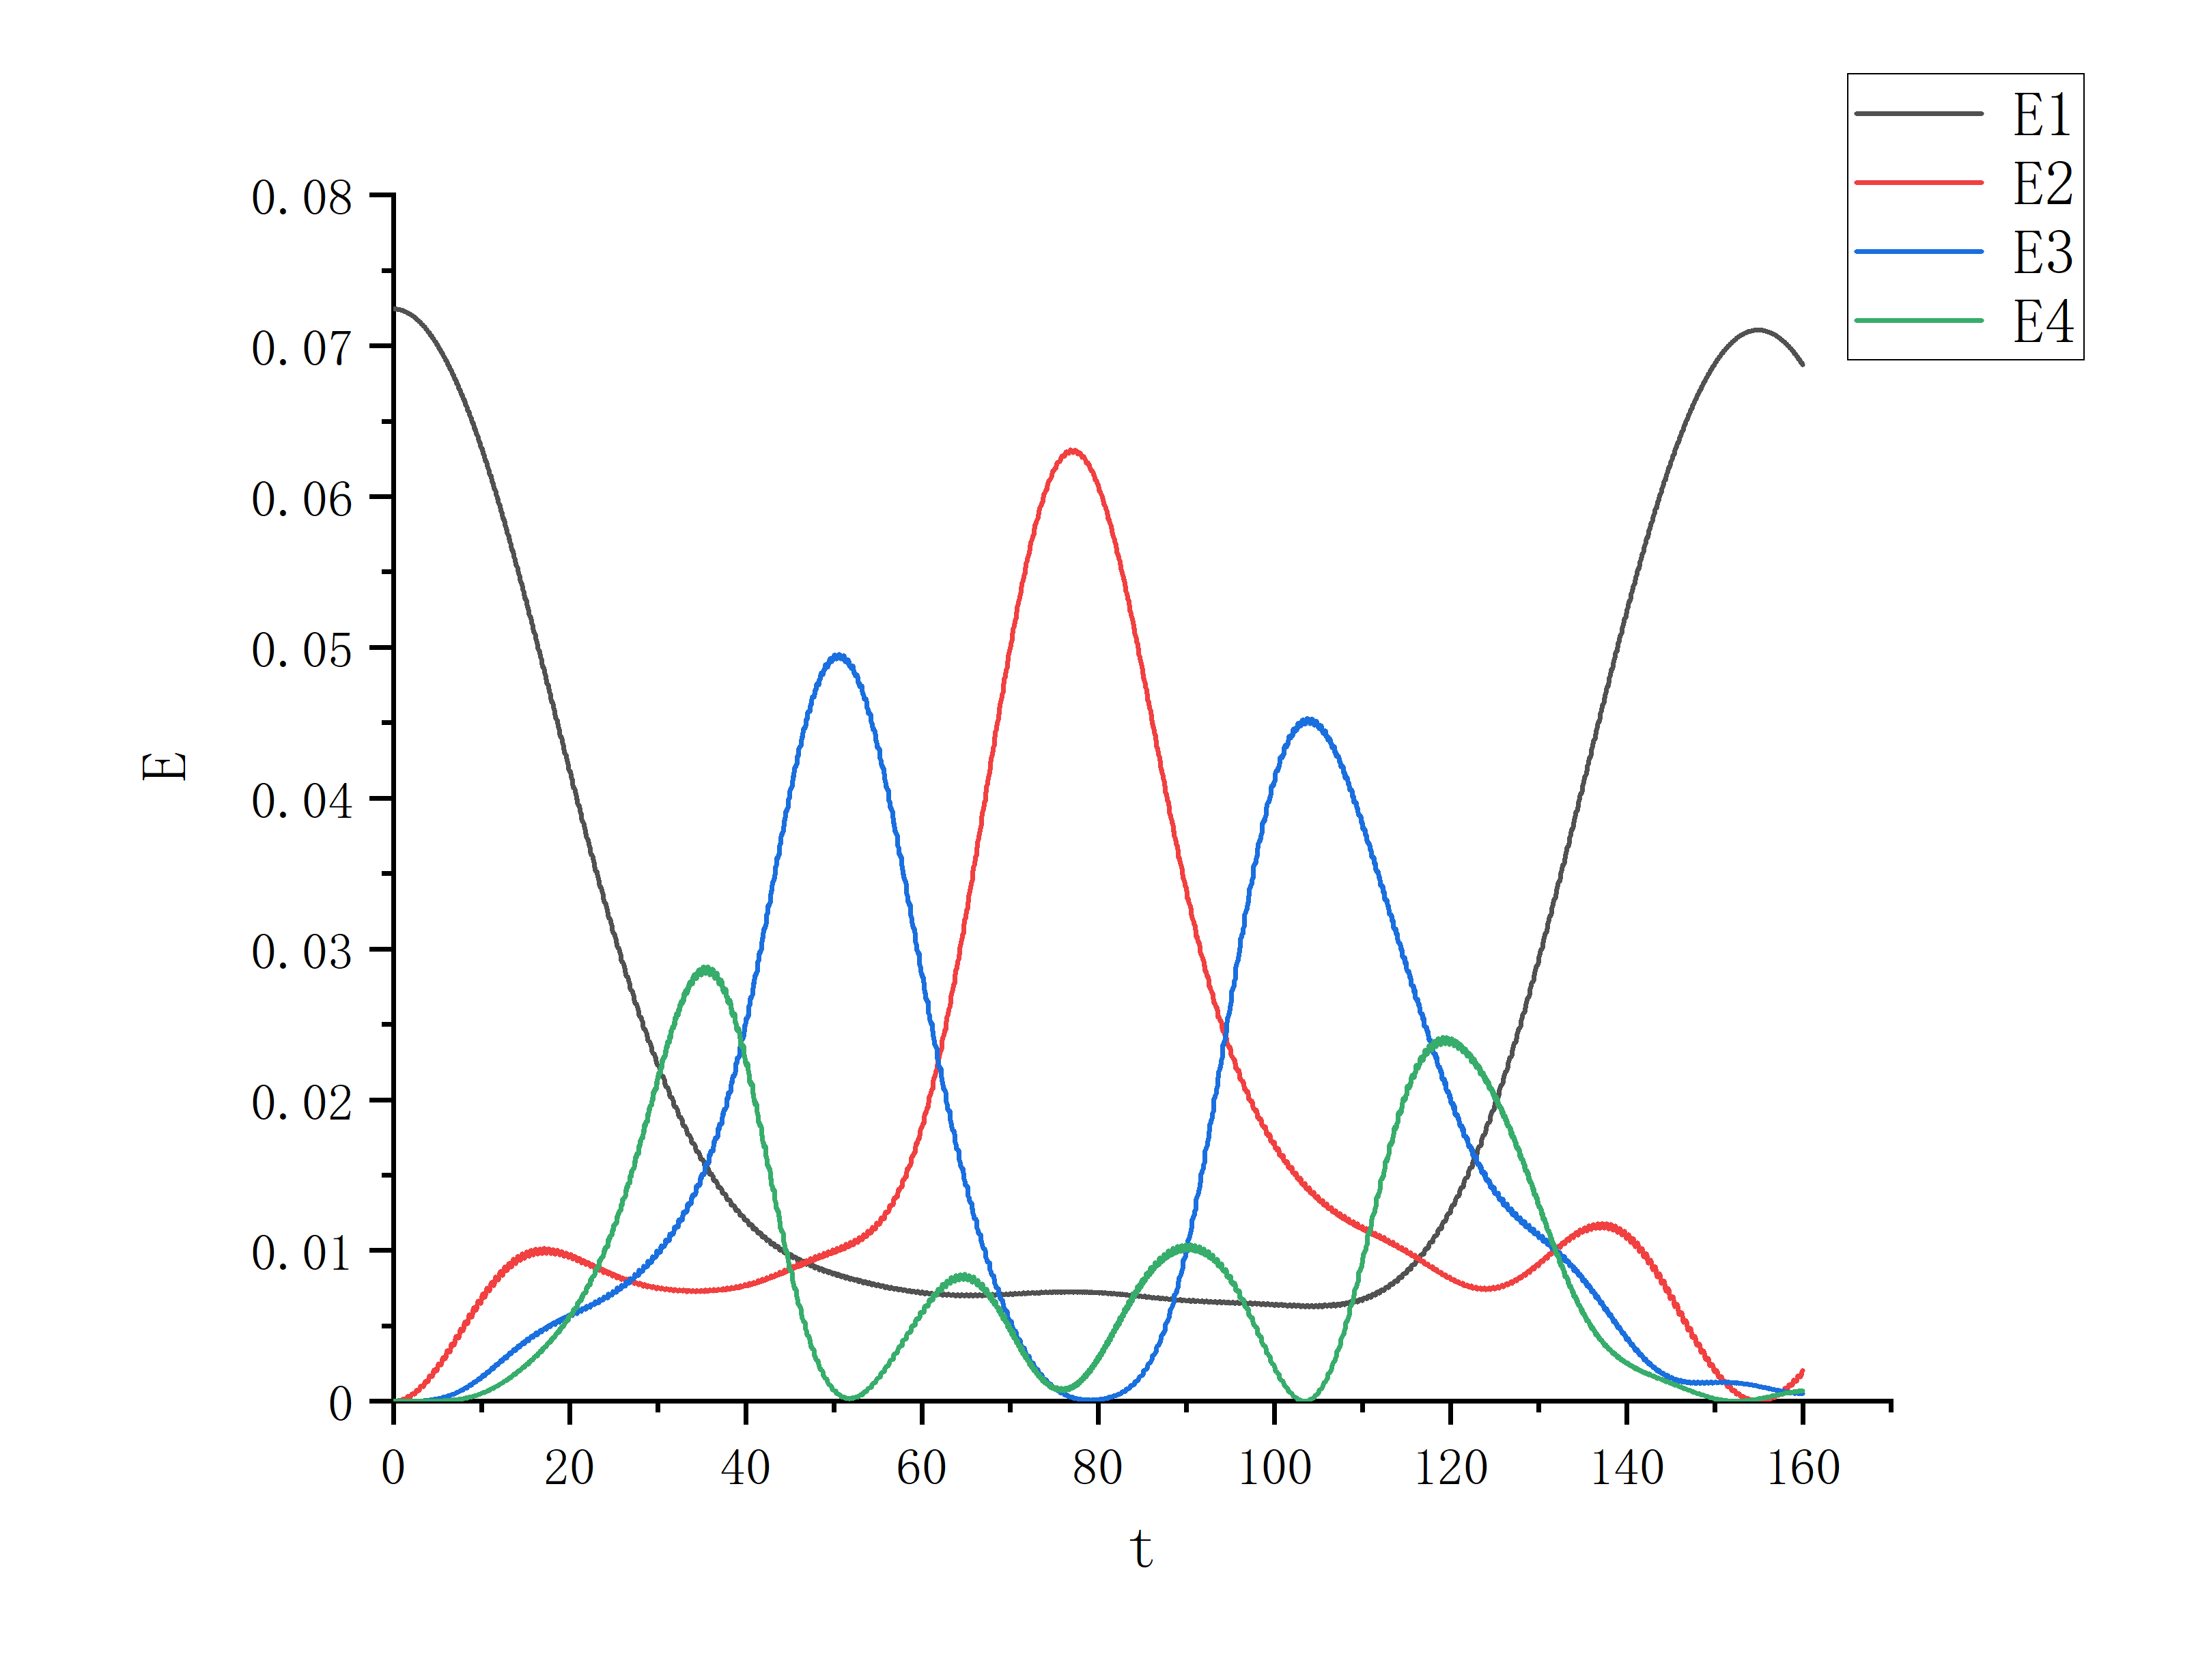
\includegraphics[width=0.8\textwidth]{第二问图.jpg}
        \caption{第二问图}\label{fig:第二问图}
    \end{figure}

    回归时刻$t=154.5$,能量比$\eta=\frac{0.071035}{0.072449}=98\%$

    \subsection{第三问}

    我们期待看到模式1逐渐弥散到其他能量模式上,最后各个模式能量基本一致,实际上却看到存在这样一个周期,体系基本回到了初态,下面提出几种可能的解释。

    \textbf{可能1:}$\alpha$不够大,非线性效应不够显著,线性效应仍然占据主导,导致能量仍然倾向于回到初始本正能量$E_1$。

    \textbf{可能2:}$n$不够大,每个弹簧非线性效应的耦合不够混乱,导致体系仍具有某种周期,就像极限情况n=1,哪怕存在非线性回复力,振子依然做周期运动。

    \textbf{可能3:}由于非线性系统的演化极大地依赖初值,这个$Q_1$初始值可能比较偶然出现了能量暂时回归的现象。

    \textbf{可能4:}体系演化时间不够长,这里虽然有高达$98\%$的能量回到初始状态,但是还是有$2\%$弥散掉了,可能让体系演化更长一段时间,会观察到能量均分的现象。

    \subsection{第四问}

    这一问与第二问求解过程几乎完全一样,只有一点点变化是体系要多演化一段时间,并且只用求每个时刻的$E_1$即可,具体代码实现见附录"q4.c"。

    这里展示$E_1$随更长的时间变化的图像。(原始数据见"q4.txt")

    \begin{figure}[H]
        \centering
        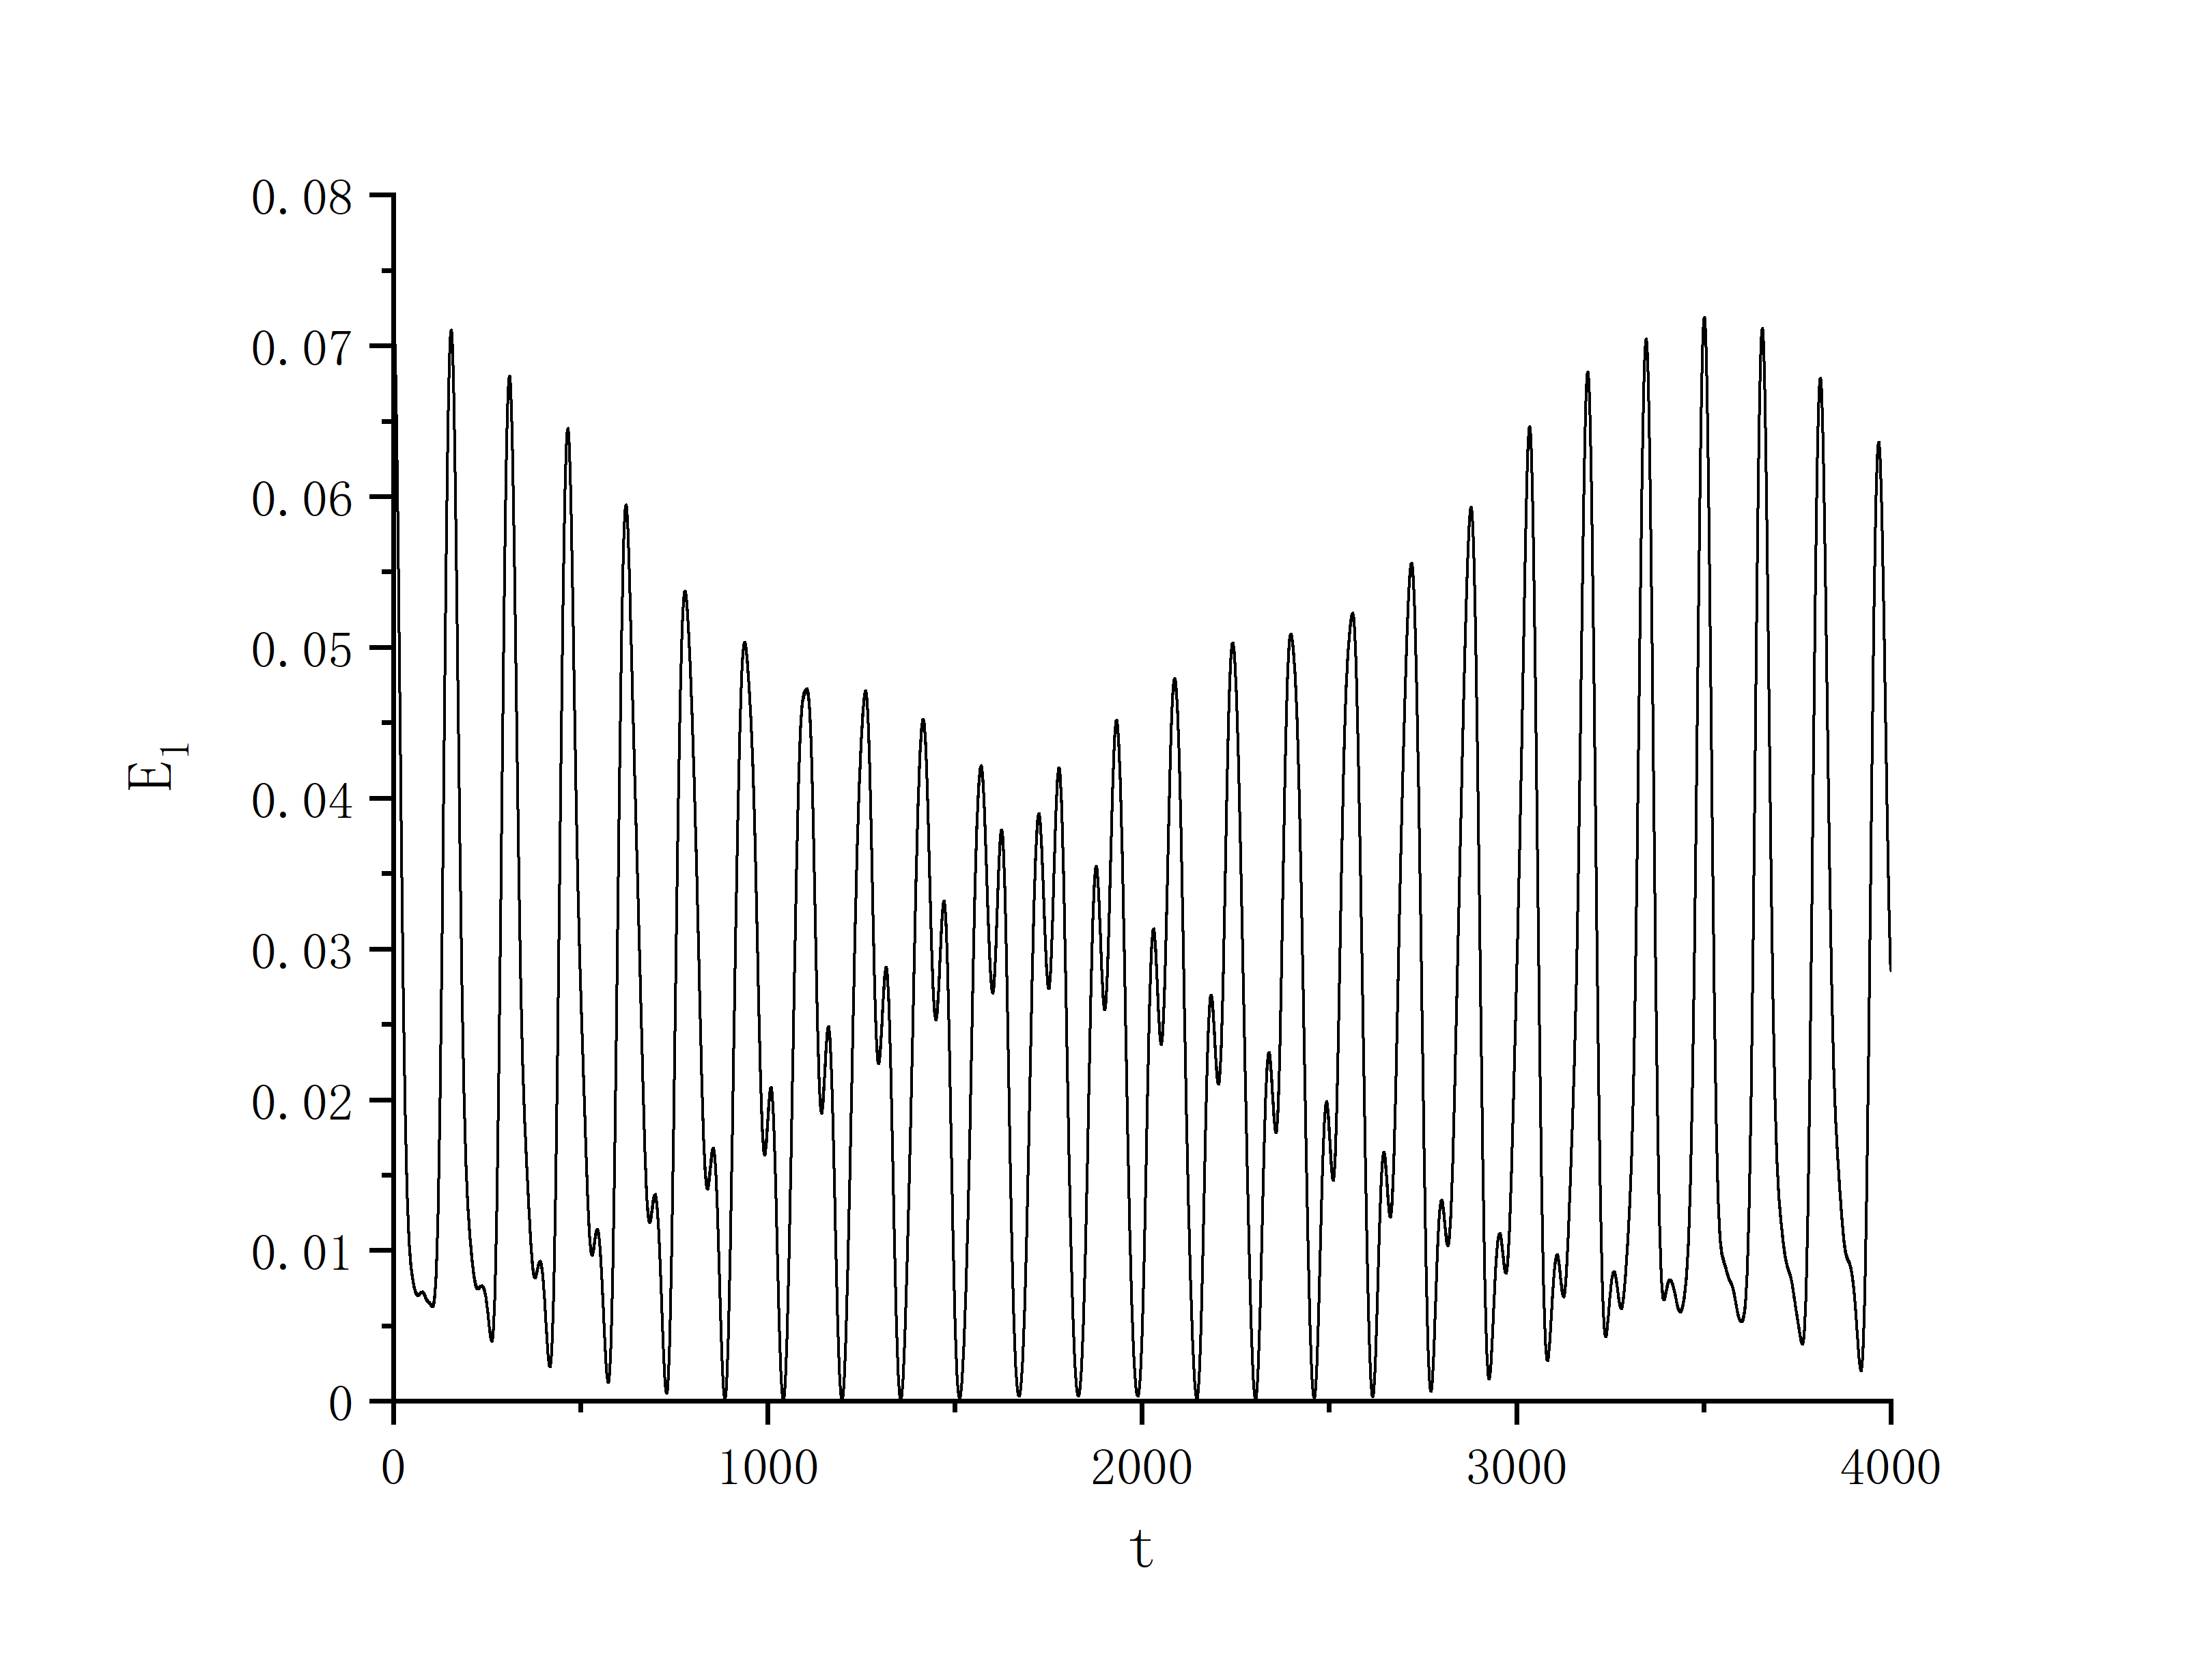
\includegraphics[width=0.8\textwidth]{第四问图.jpg}
        \caption{第四问图}\label{fig:第四问图}
    \end{figure}

    回归时刻$t=3502.18$,能量比例$\eta=\frac{0.071902}{0.072449}=99\%$

    \subsection{第五问}

    本问与前问求解过程基本一致,为探究各个模式能量随时间的变化。我们取t的单位仍为$2\pi/\omega_1$,每隔0.01计算一次全部32个模式的能量。同时,为比较不同初始条件下体系演化形式的不同,我们分别就$Q_1(0)=20$和$Q_1(0)=4$分别计算t从0至4000中所有模式能量的演化。具体代码实现见附录"q5.c"。运行结果$Q_1(0)=20$对应"q5_sparsify.txt",$Q_1(0)=4$对应"q5_cmp_sparsify.txt"。

    接下来,我们完全可以选择将数据导入origin,再绘制64幅"E-t"图,但这样十分耗时耗力。我们选择运用python的numpy和matplotlib包可以实现从txt读取数据、画图并保存。具体代码实现见附录"plotTool.py"。

    下面展示两种初始条件所有模式能量随时间的演化图。其中左侧是初态$Q_1(0)=4$的体系,右侧是初态$Q_1(0)=20$的体系,由上到下分别是$E_1$到$E_{32}$随时间的演化。

    \begin{figure}[H]
        \begin{minipage}[t]{0.49\textwidth}
            \centering
            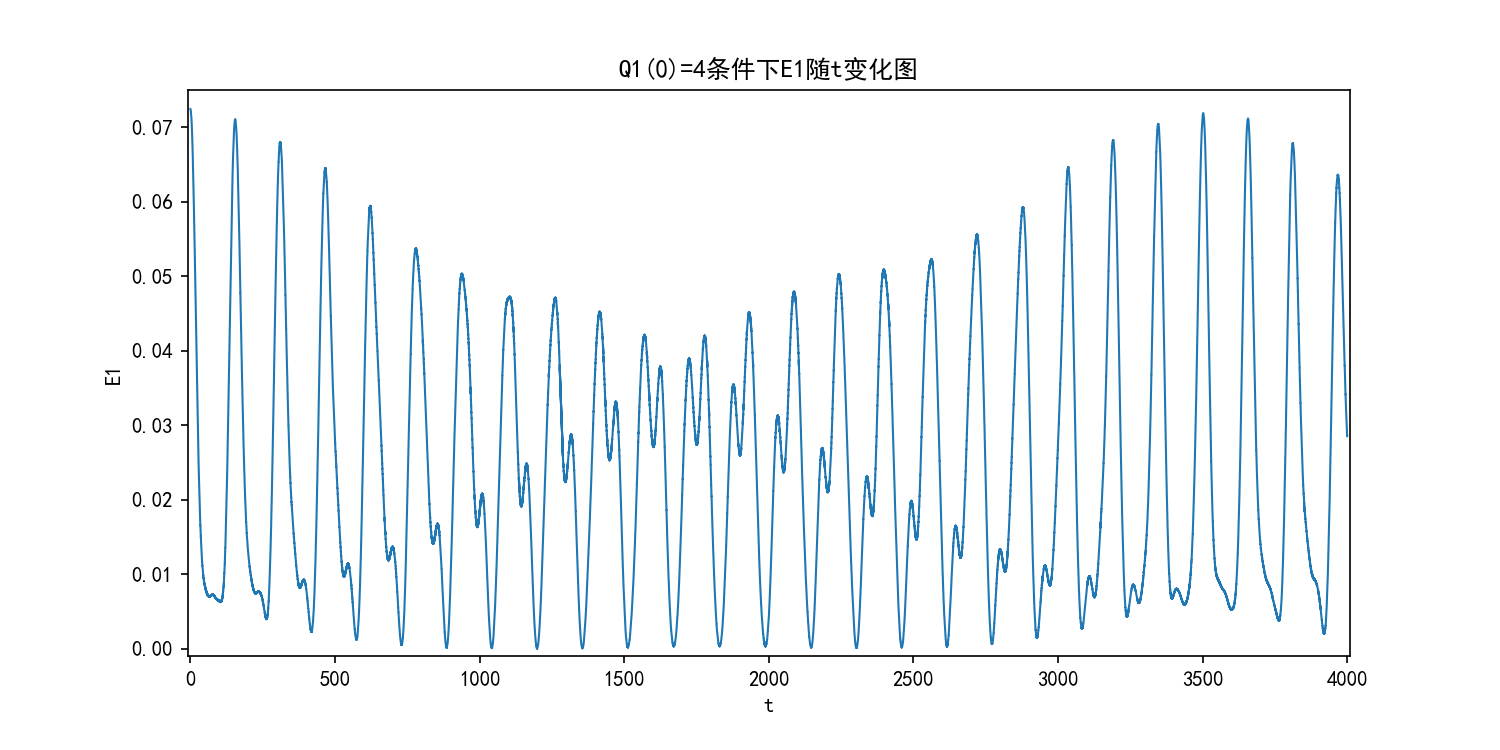
\includegraphics[width=\textwidth]{./q5_pics/cmp/E1.png}
        \end{minipage}
        \begin{minipage}[t]{0.49\textwidth}
            \centering
            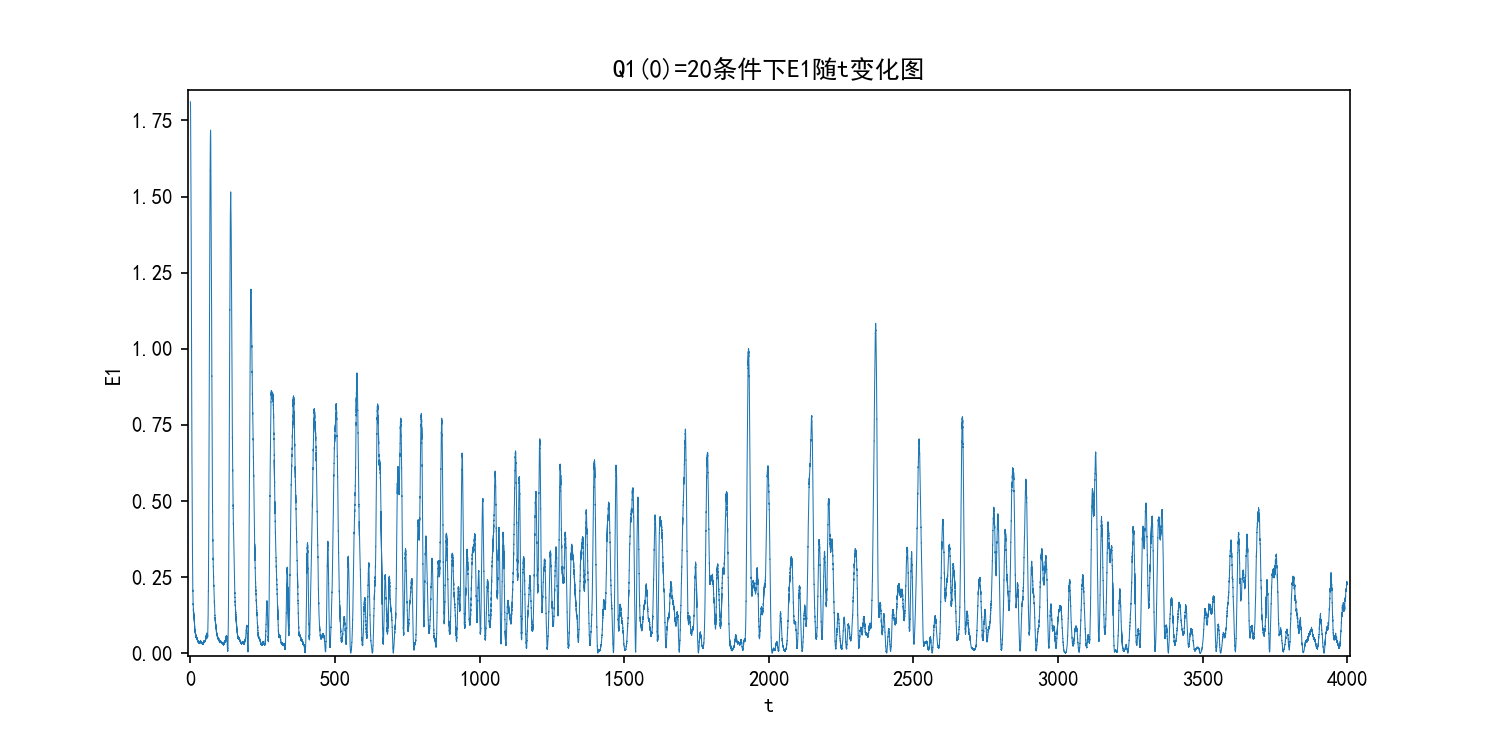
\includegraphics[width=\textwidth]{./q5_pics/exp/E1.png}
        \end{minipage}
        \caption{E1}\label{fig:E1 in q5}
    \end{figure}
    \begin{figure}[H]
        \begin{minipage}[t]{0.49\textwidth}
            \centering
            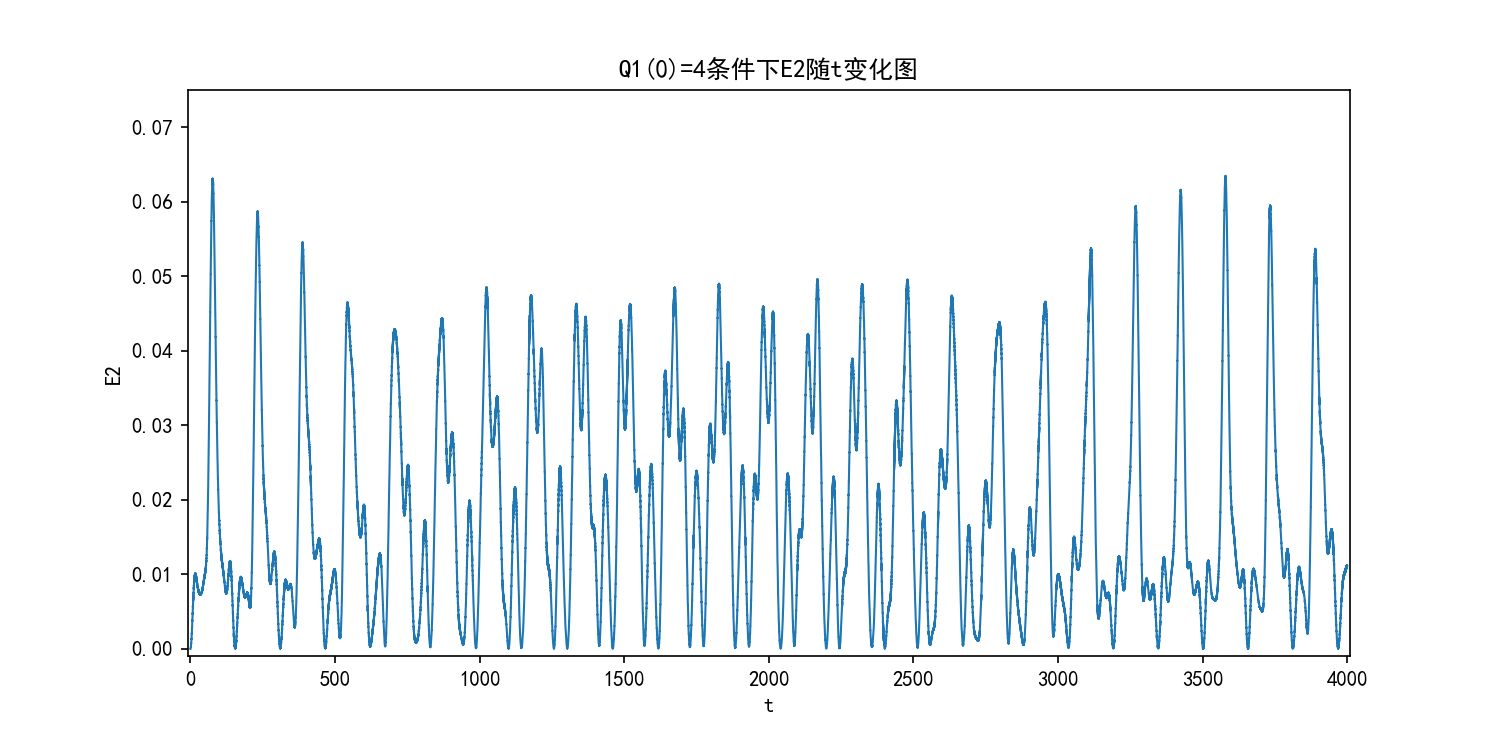
\includegraphics[width=\textwidth]{./q5_pics/cmp/E2.png}
        \end{minipage}
        \begin{minipage}[t]{0.49\textwidth}
            \centering
            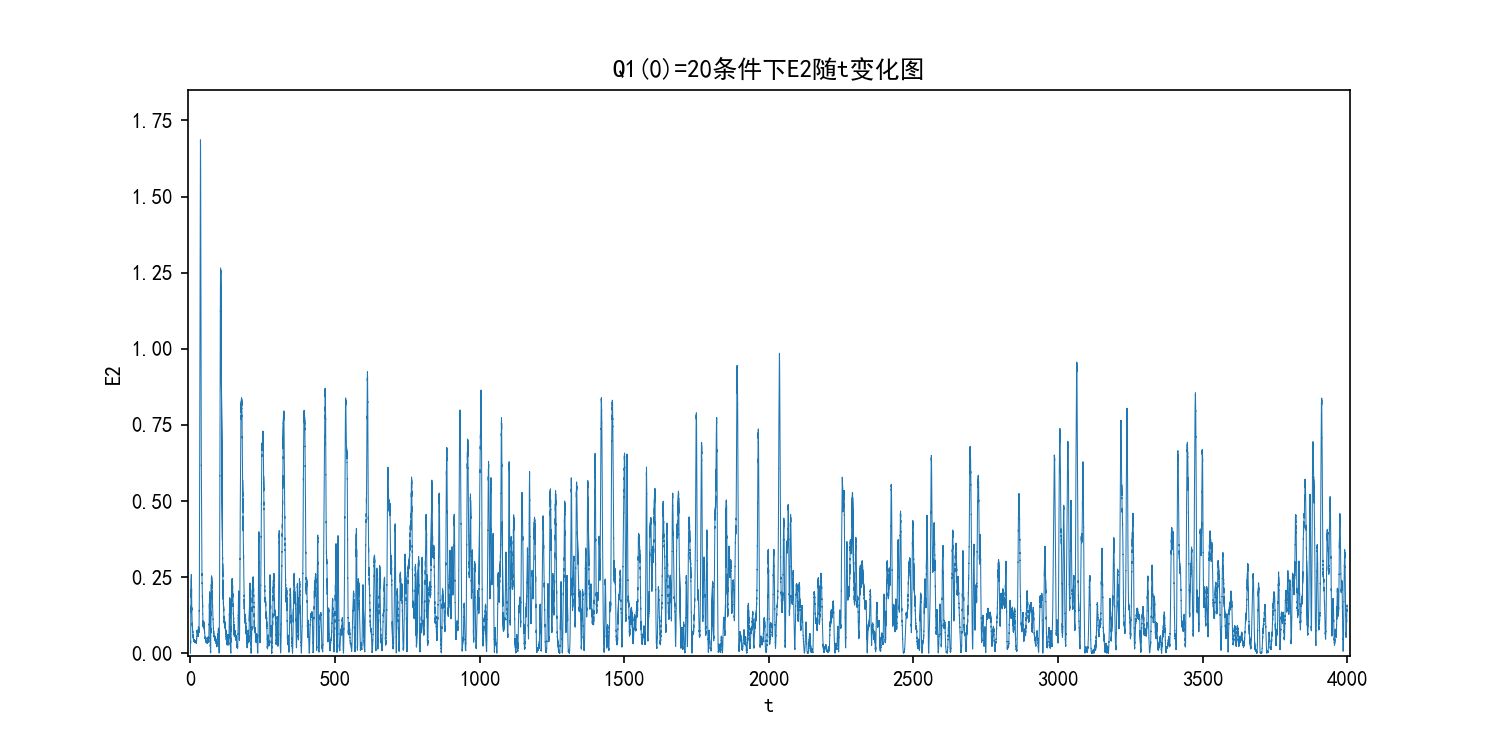
\includegraphics[width=\textwidth]{./q5_pics/exp/E2.png}
        \end{minipage}
        \caption{E2}\label{fig:E2 in q5}
    \end{figure}
    \begin{figure}[H]
        \begin{minipage}[t]{0.49\textwidth}
            \centering
            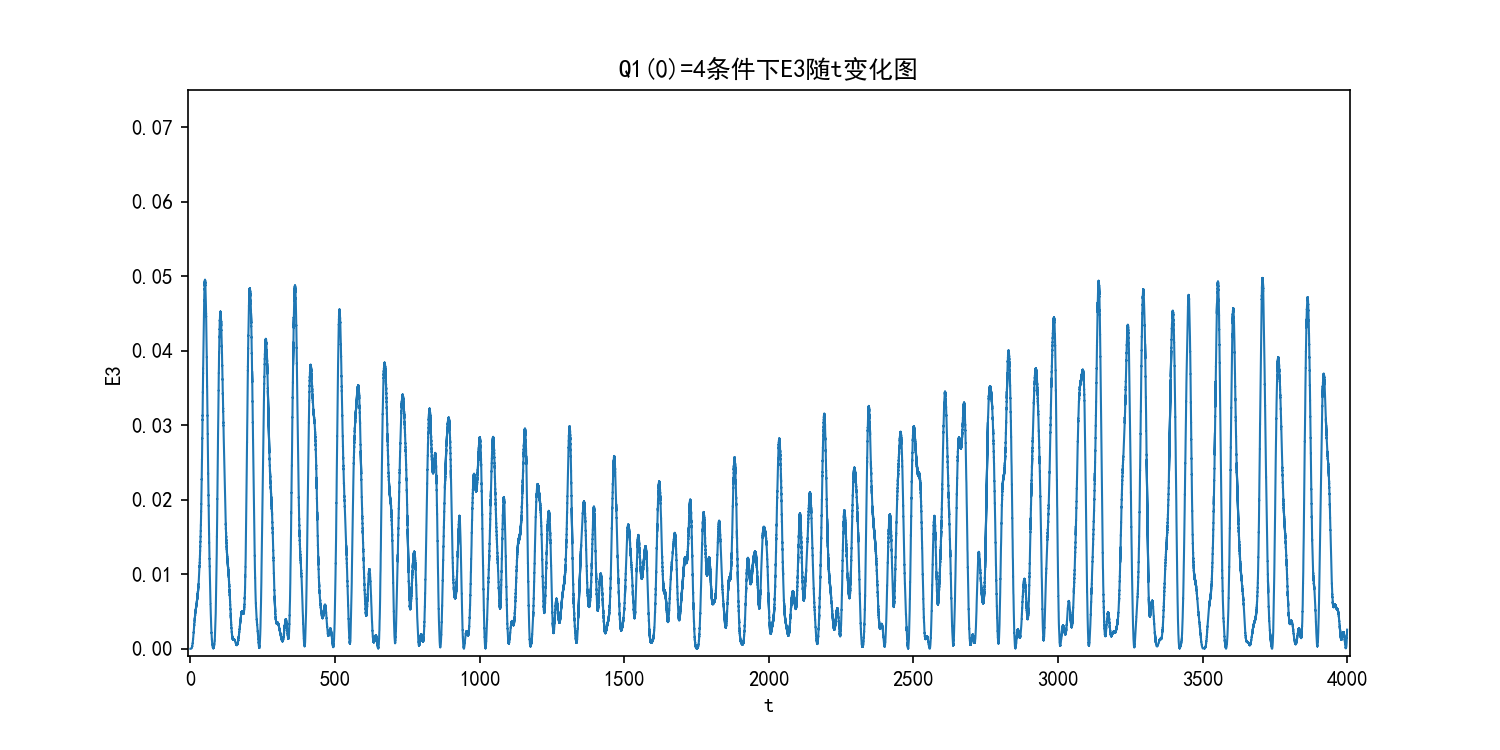
\includegraphics[width=\textwidth]{./q5_pics/cmp/E3.png}
        \end{minipage}
        \begin{minipage}[t]{0.49\textwidth}
            \centering
            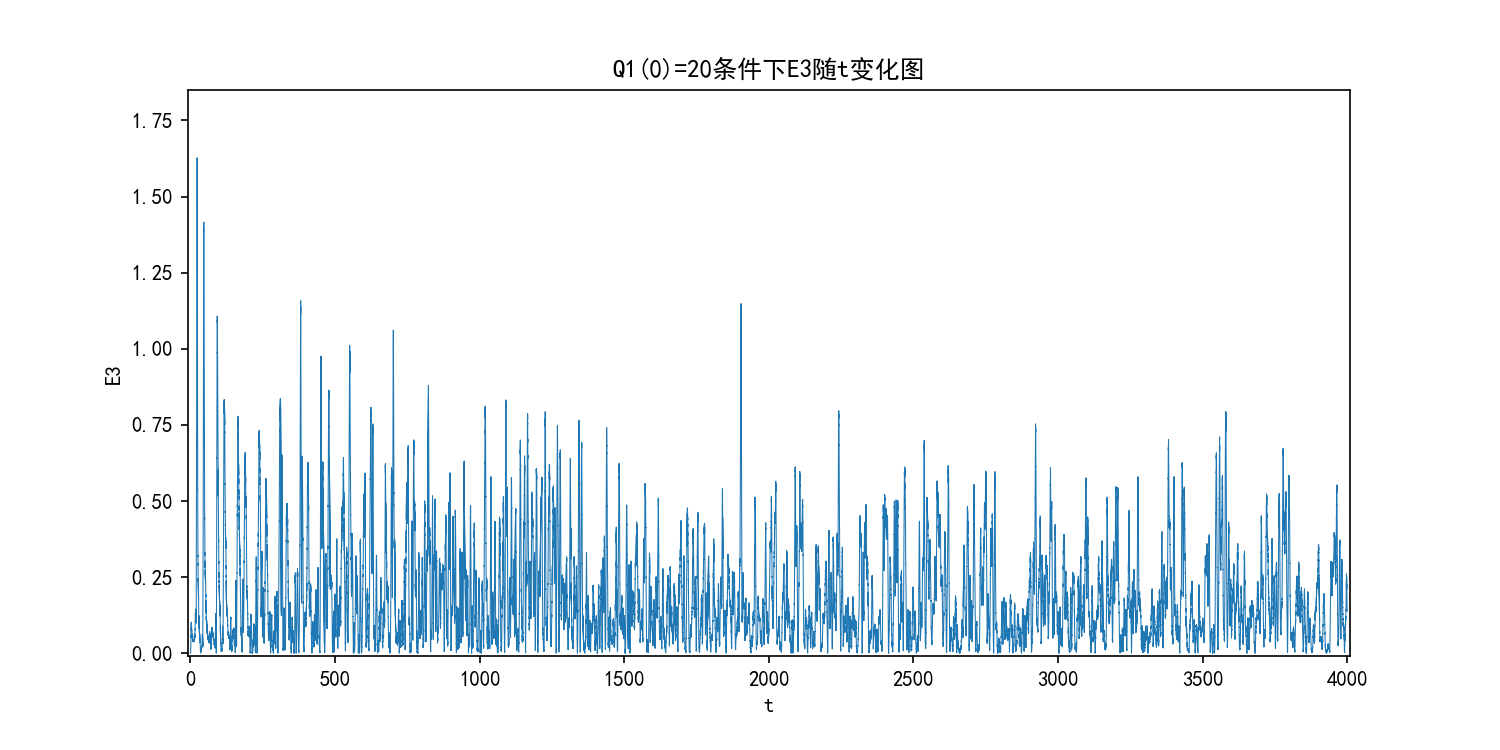
\includegraphics[width=\textwidth]{./q5_pics/exp/E3.png}
        \end{minipage}
        \caption{E3}\label{fig:E3 in q5}
    \end{figure}
    \begin{figure}[H]
        \begin{minipage}[t]{0.49\textwidth}
            \centering
            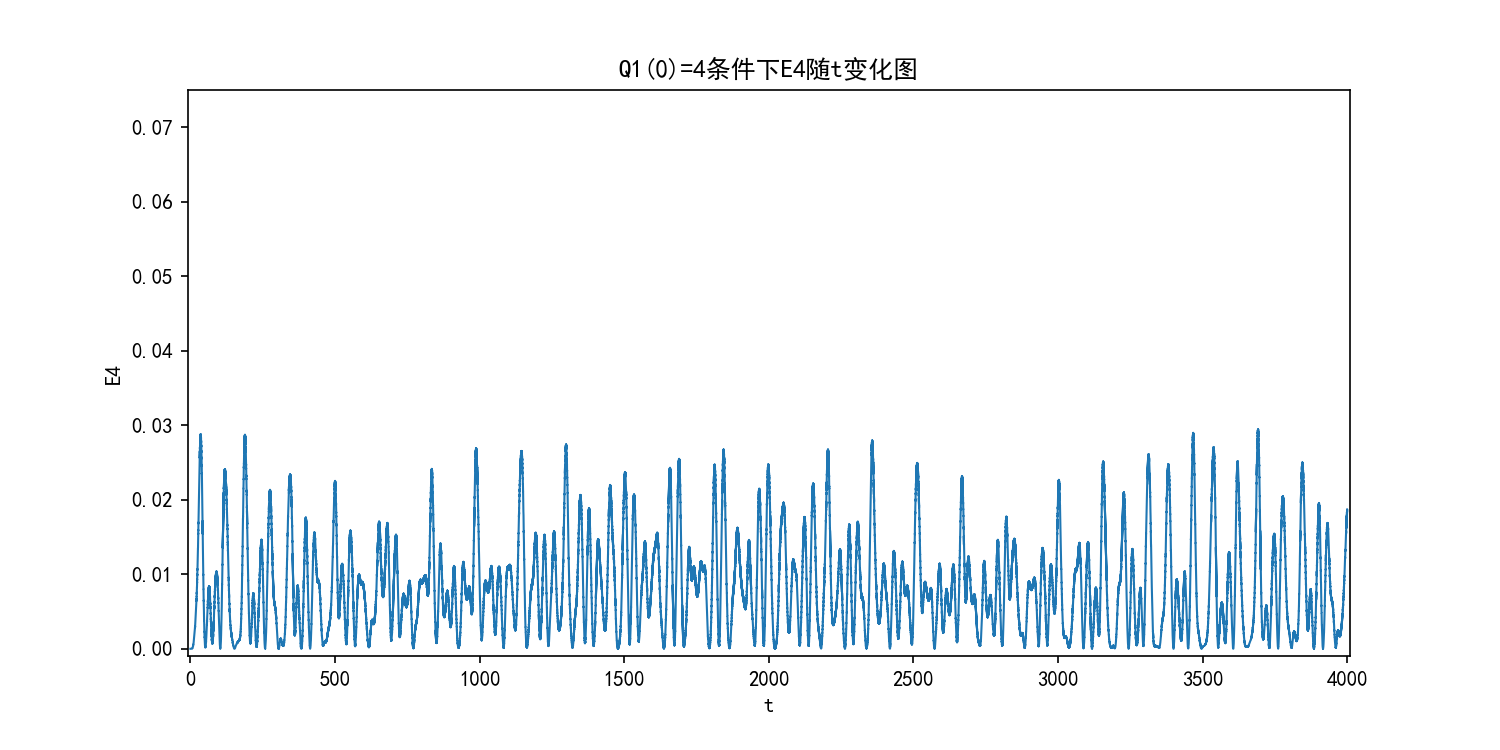
\includegraphics[width=\textwidth]{./q5_pics/cmp/E4.png}
        \end{minipage}
        \begin{minipage}[t]{0.49\textwidth}
            \centering
            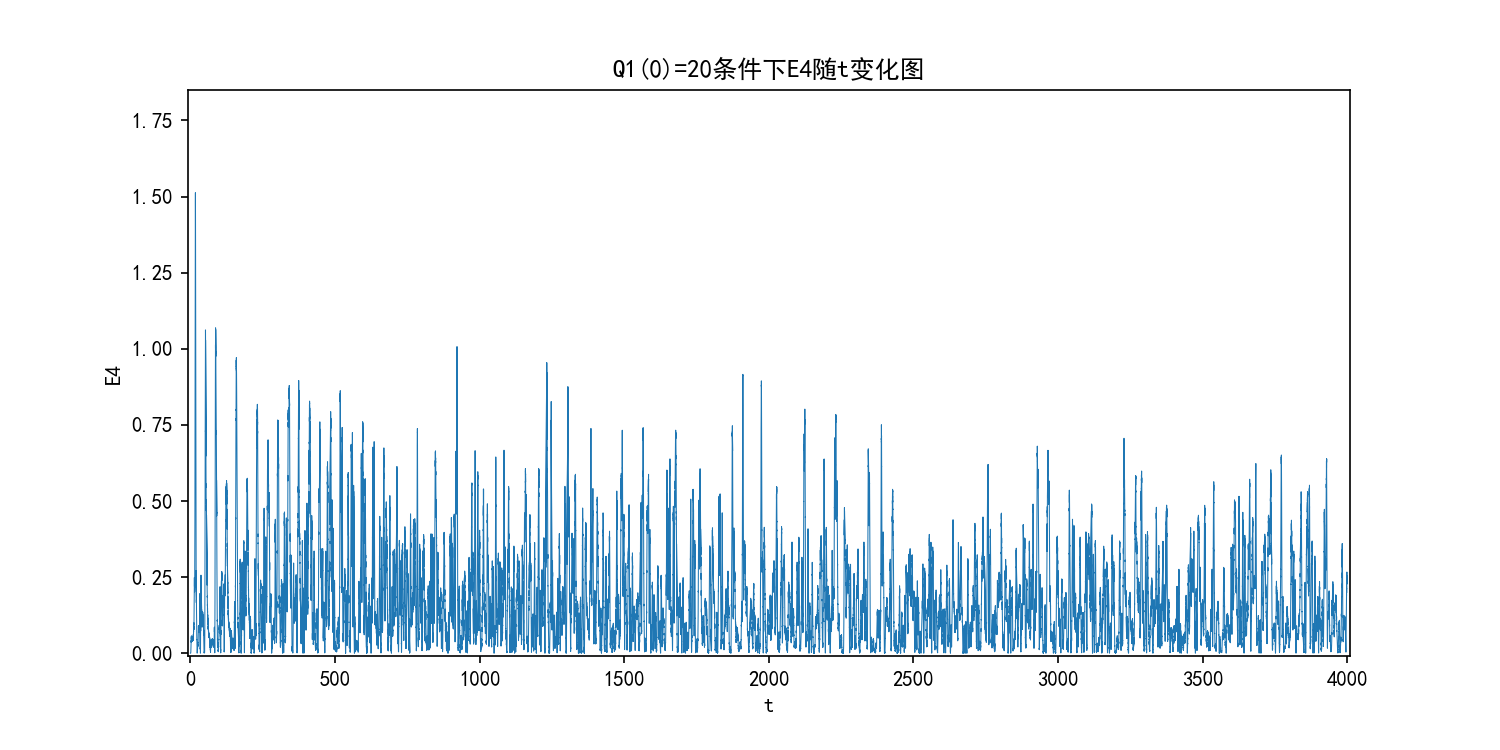
\includegraphics[width=\textwidth]{./q5_pics/exp/E4.png}
        \end{minipage}
        \caption{E4}\label{fig:E4 in q5}
    \end{figure}
    \begin{figure}[H]
        \begin{minipage}[t]{0.49\textwidth}
            \centering
            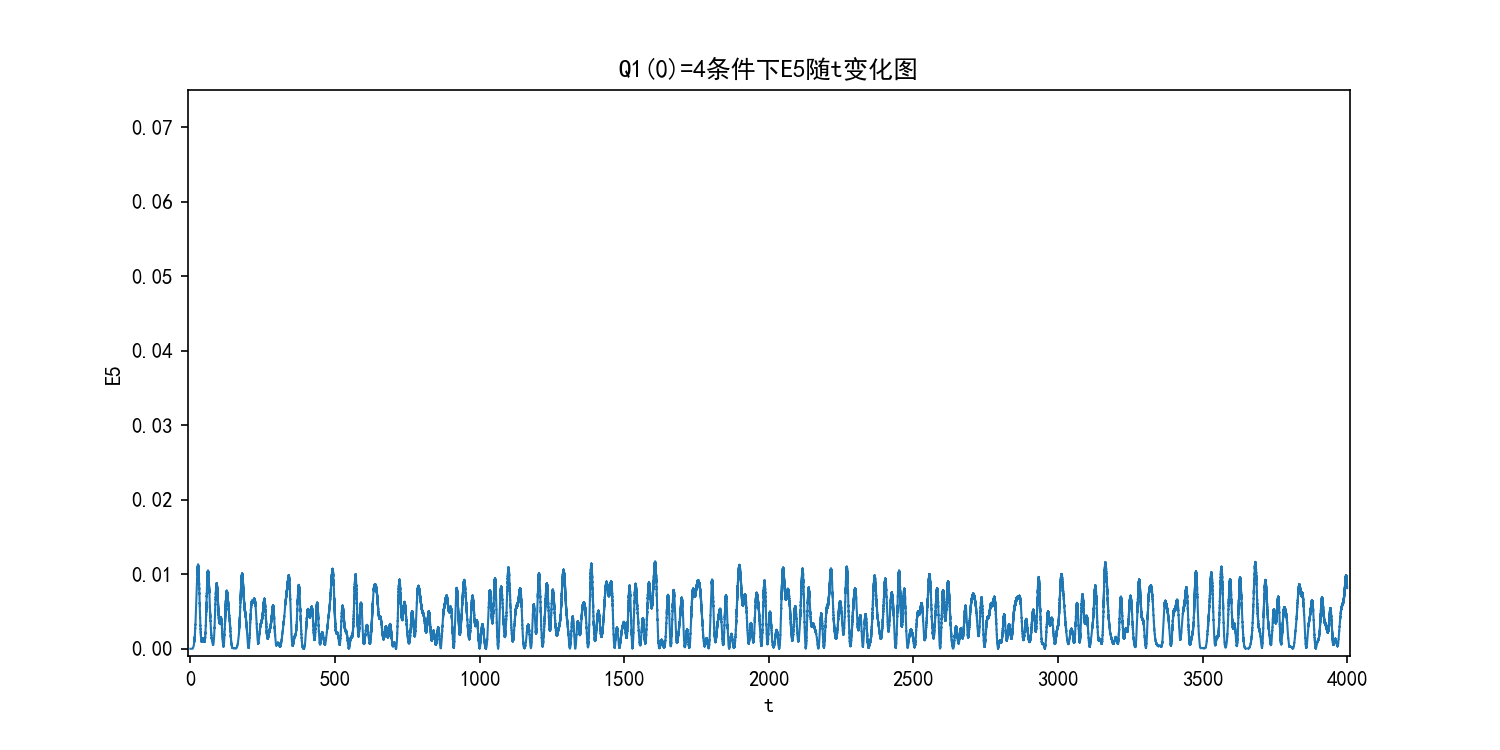
\includegraphics[width=\textwidth]{./q5_pics/cmp/E5.png}
        \end{minipage}
        \begin{minipage}[t]{0.49\textwidth}
            \centering
            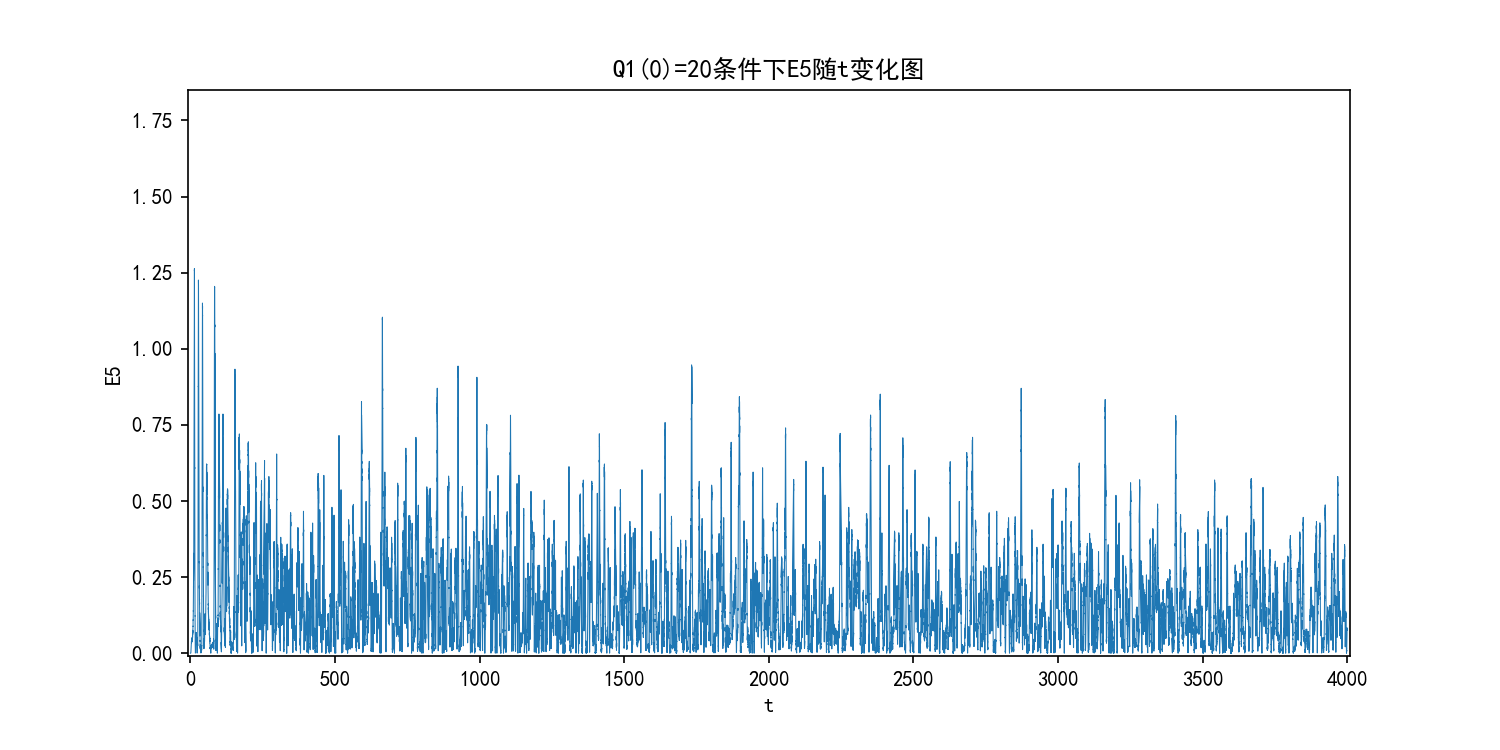
\includegraphics[width=\textwidth]{./q5_pics/exp/E5.png}
        \end{minipage}
        \caption{E5}\label{fig:E5 in q5}
    \end{figure}
    \begin{figure}[H]
        \begin{minipage}[t]{0.49\textwidth}
            \centering
            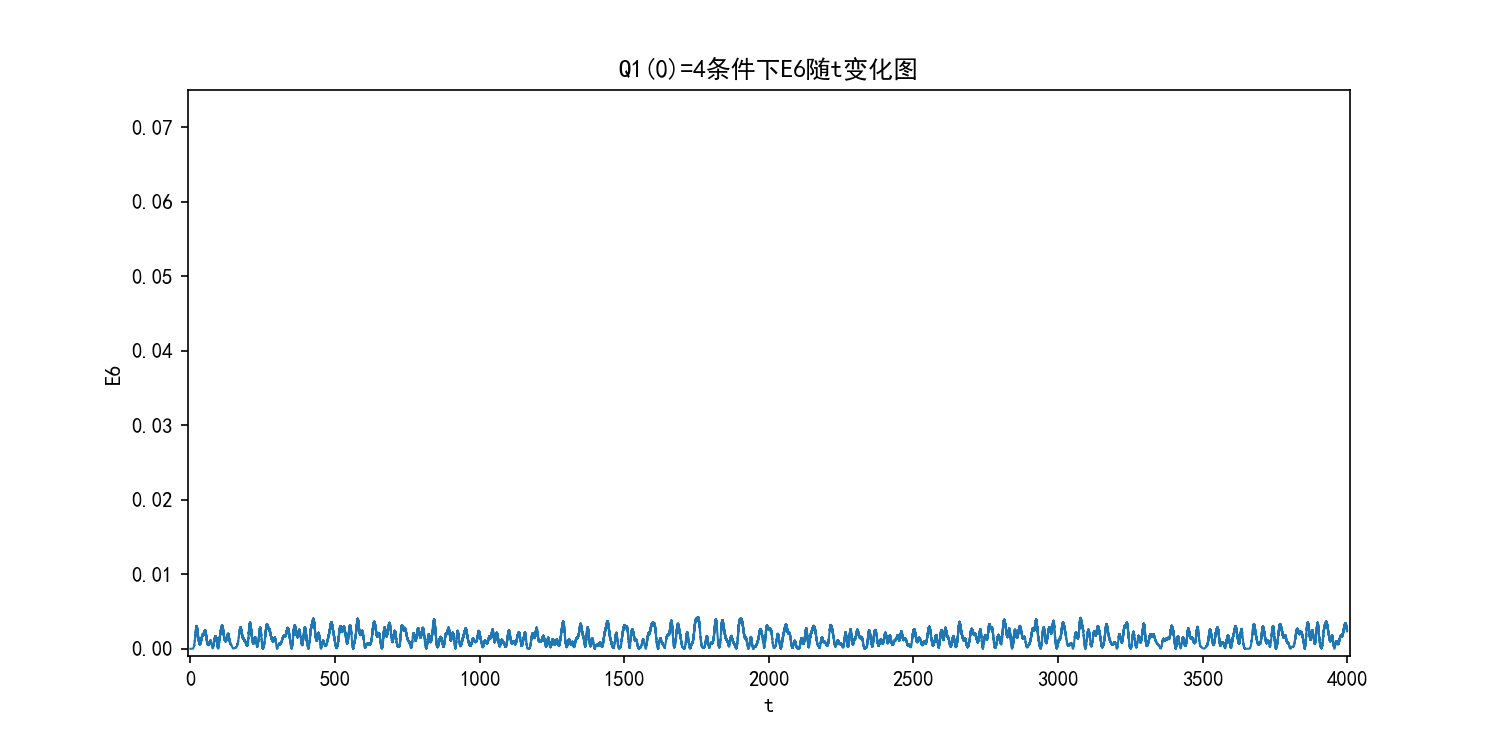
\includegraphics[width=\textwidth]{./q5_pics/cmp/E6.png}
        \end{minipage}
        \begin{minipage}[t]{0.49\textwidth}
            \centering
            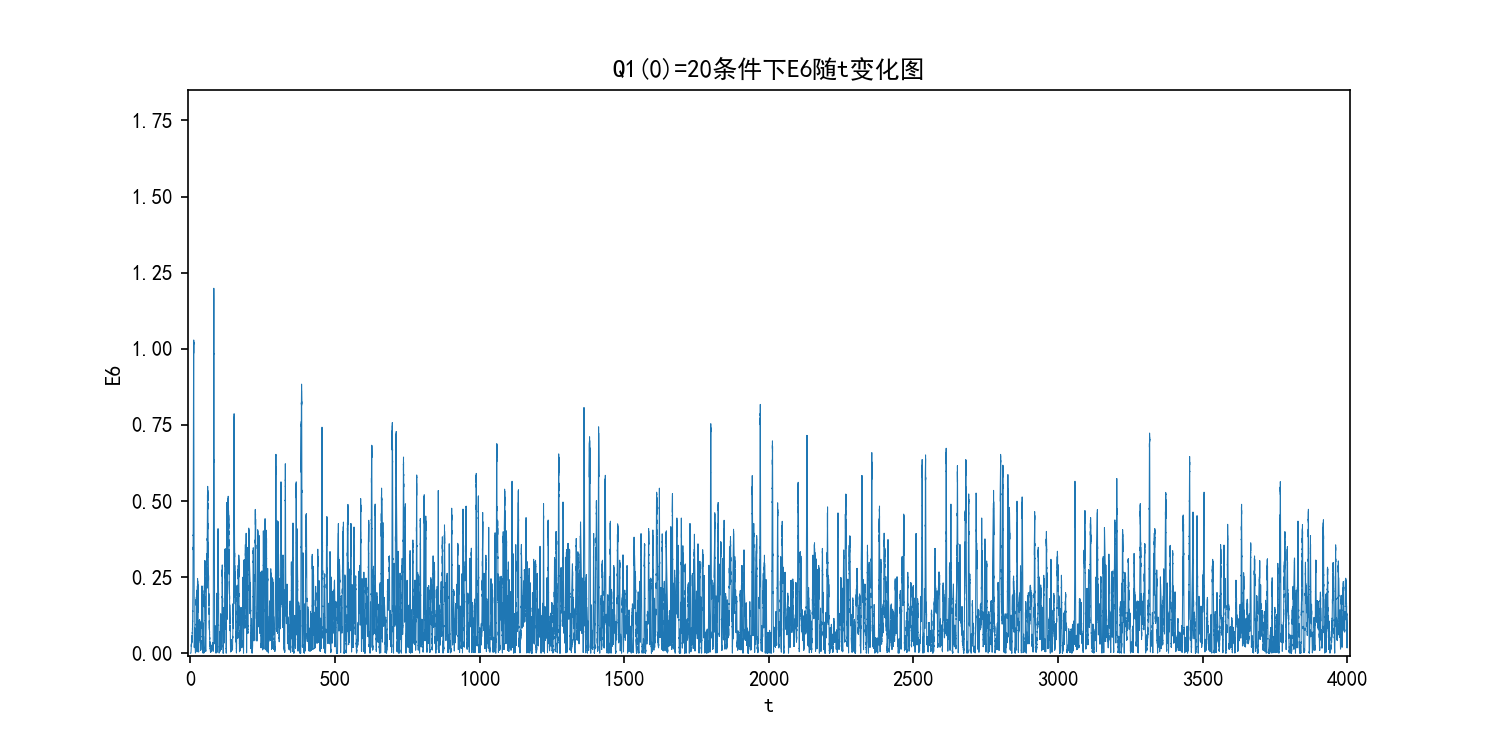
\includegraphics[width=\textwidth]{./q5_pics/exp/E6.png}
        \end{minipage}
        \caption{E6}\label{fig:E6 in q5}
    \end{figure}
    \begin{figure}[H]
        \begin{minipage}[t]{0.49\textwidth}
            \centering
            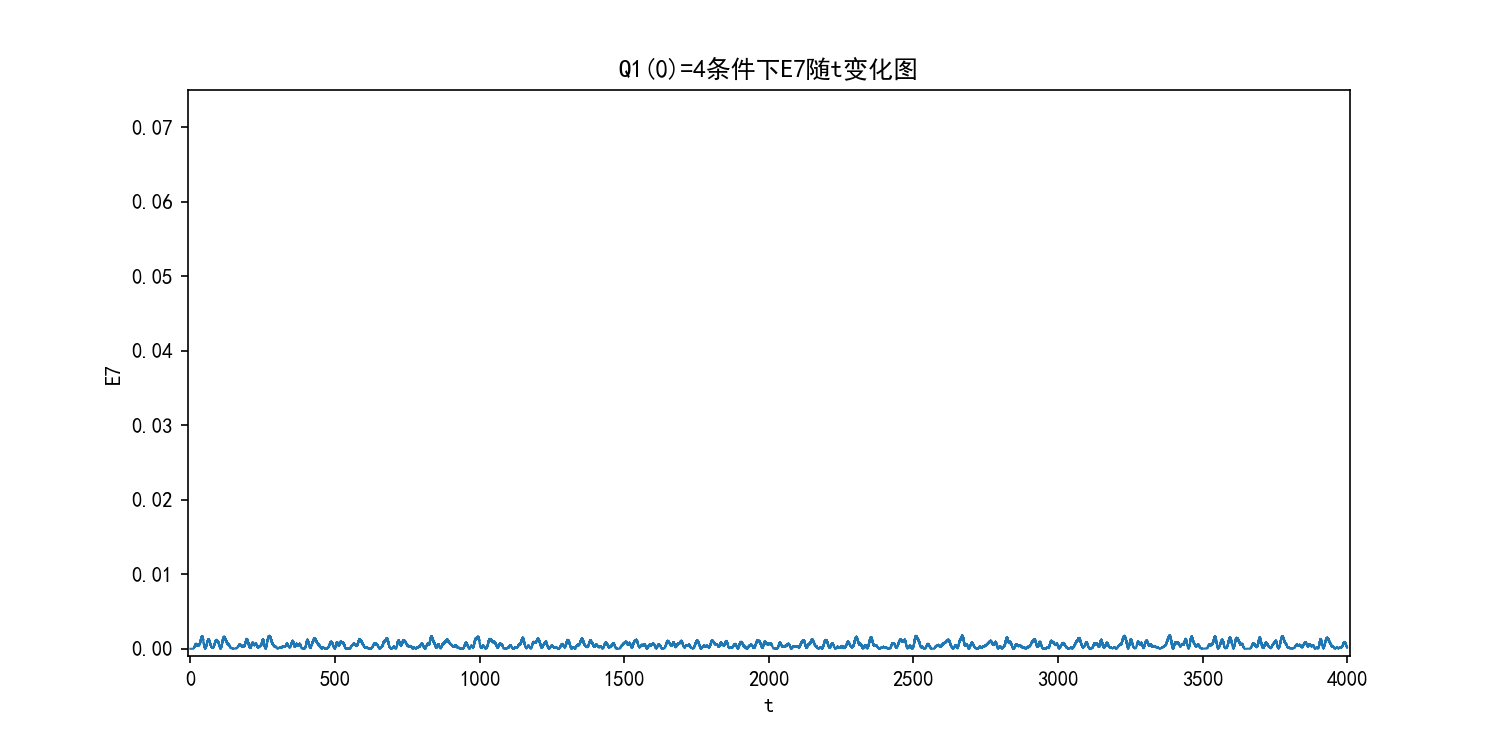
\includegraphics[width=\textwidth]{./q5_pics/cmp/E7.png}
        \end{minipage}
        \begin{minipage}[t]{0.49\textwidth}
            \centering
            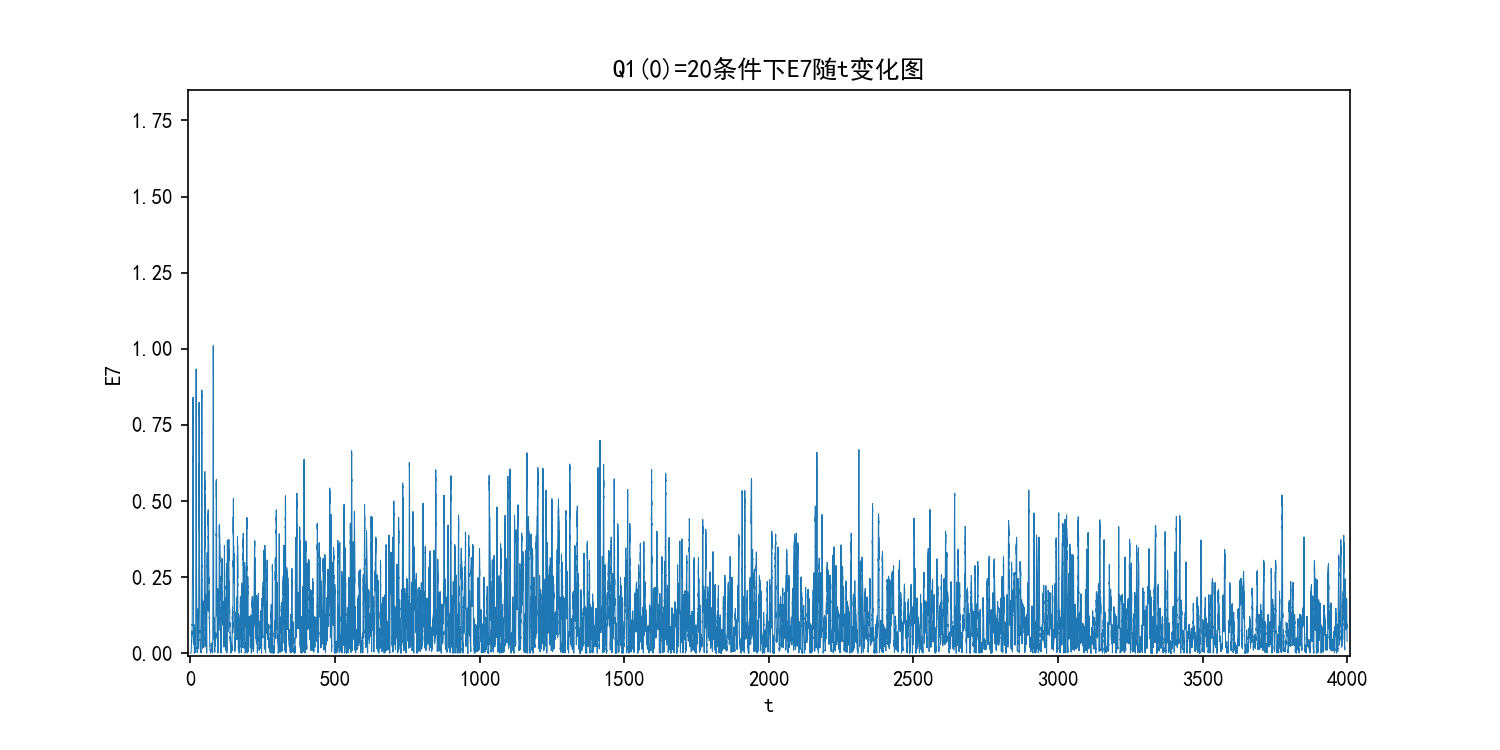
\includegraphics[width=\textwidth]{./q5_pics/exp/E7.png}
        \end{minipage}
        \caption{E7}\label{fig:E7 in q5}
    \end{figure}
    \begin{figure}[H]
        \begin{minipage}[t]{0.49\textwidth}
            \centering
            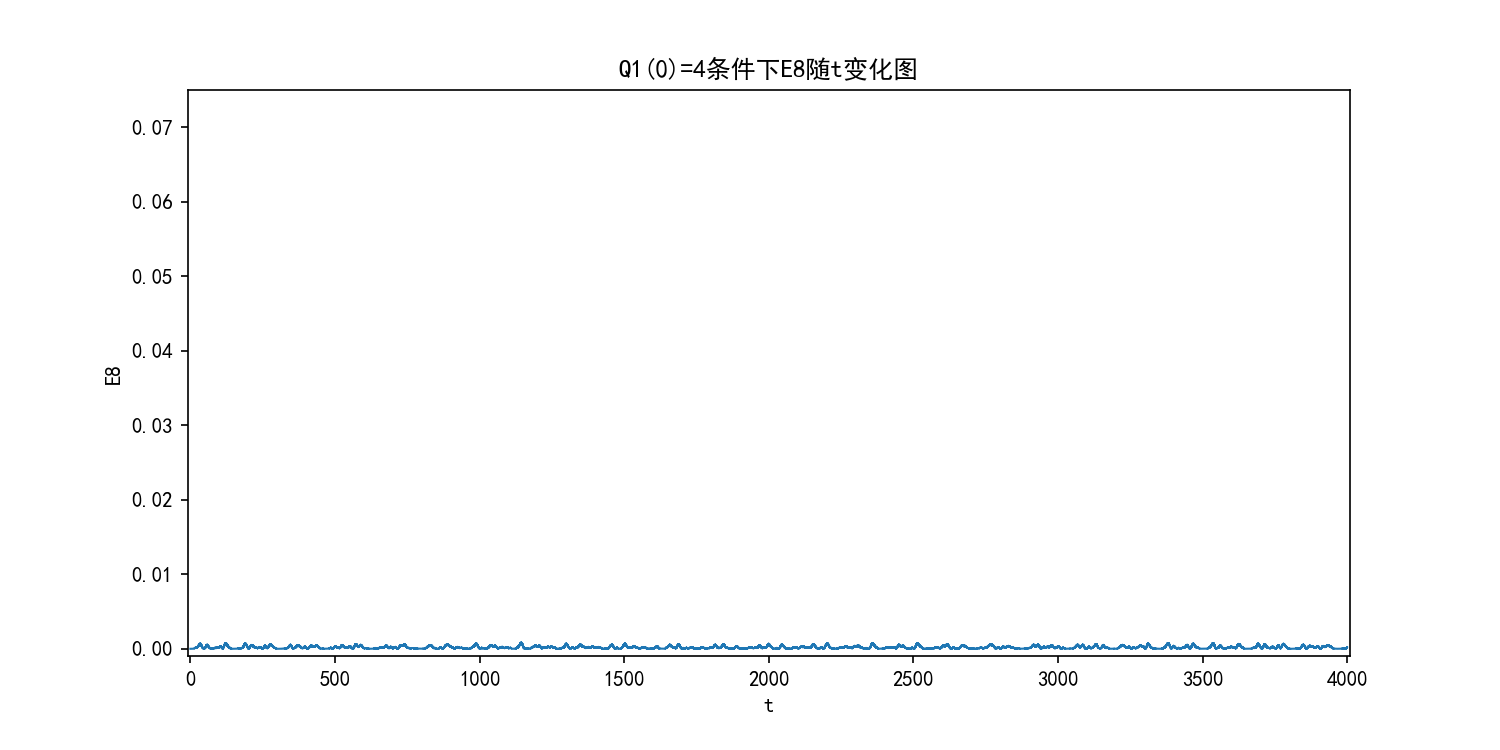
\includegraphics[width=\textwidth]{./q5_pics/cmp/E8.png}
        \end{minipage}
        \begin{minipage}[t]{0.49\textwidth}
            \centering
            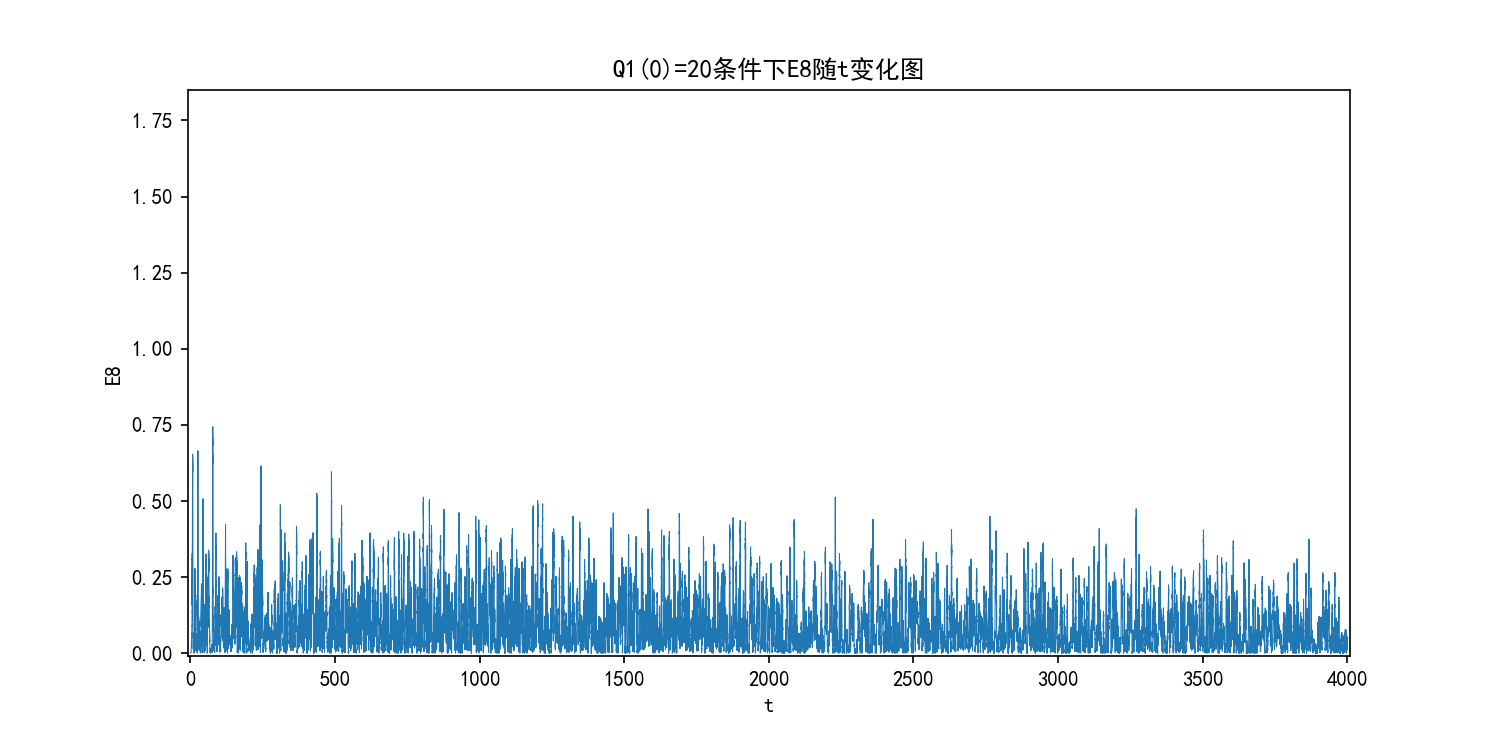
\includegraphics[width=\textwidth]{./q5_pics/exp/E8.png}
        \end{minipage}
        \caption{E8}\label{fig:E8 in q5}
    \end{figure}
    \begin{figure}[H]
        \begin{minipage}[t]{0.49\textwidth}
            \centering
            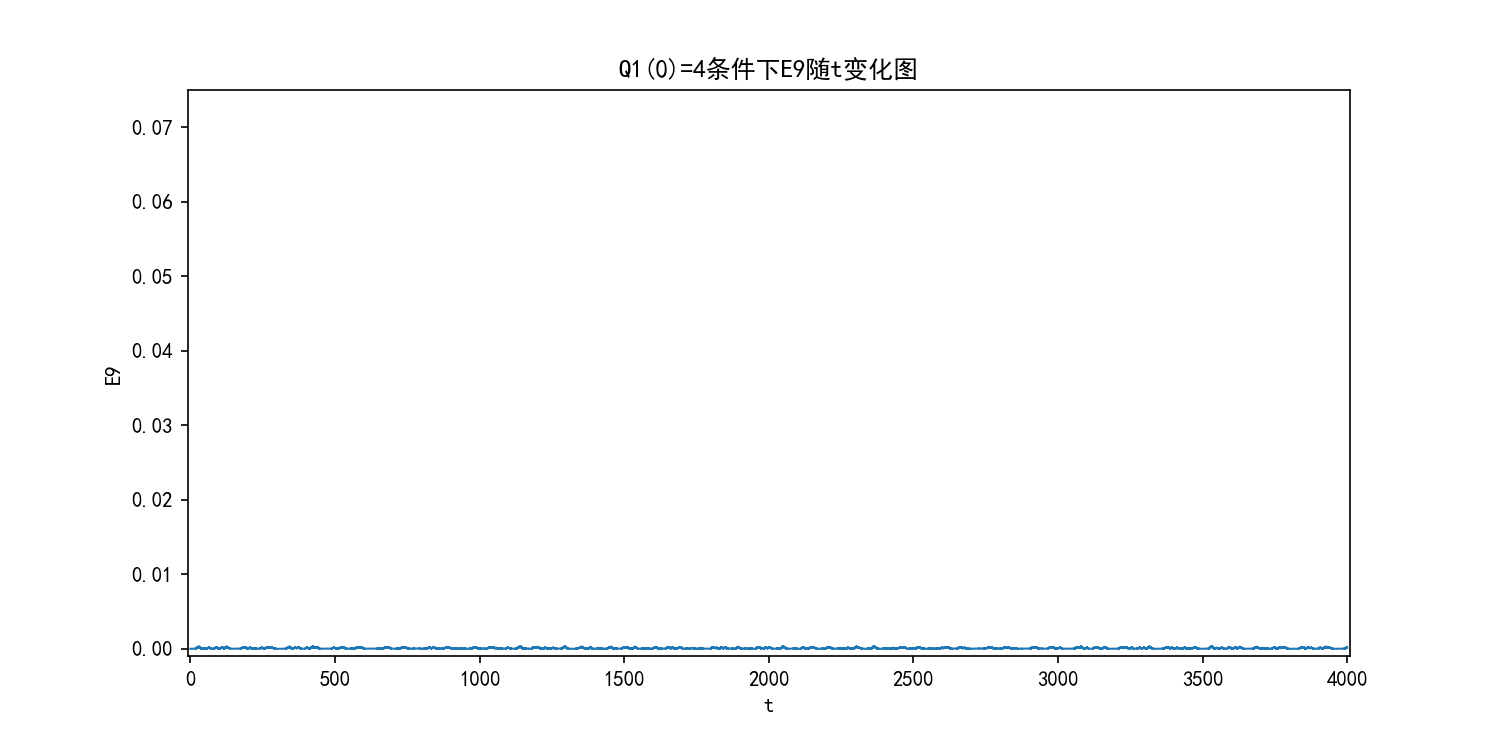
\includegraphics[width=\textwidth]{./q5_pics/cmp/E9.png}
        \end{minipage}
        \begin{minipage}[t]{0.49\textwidth}
            \centering
            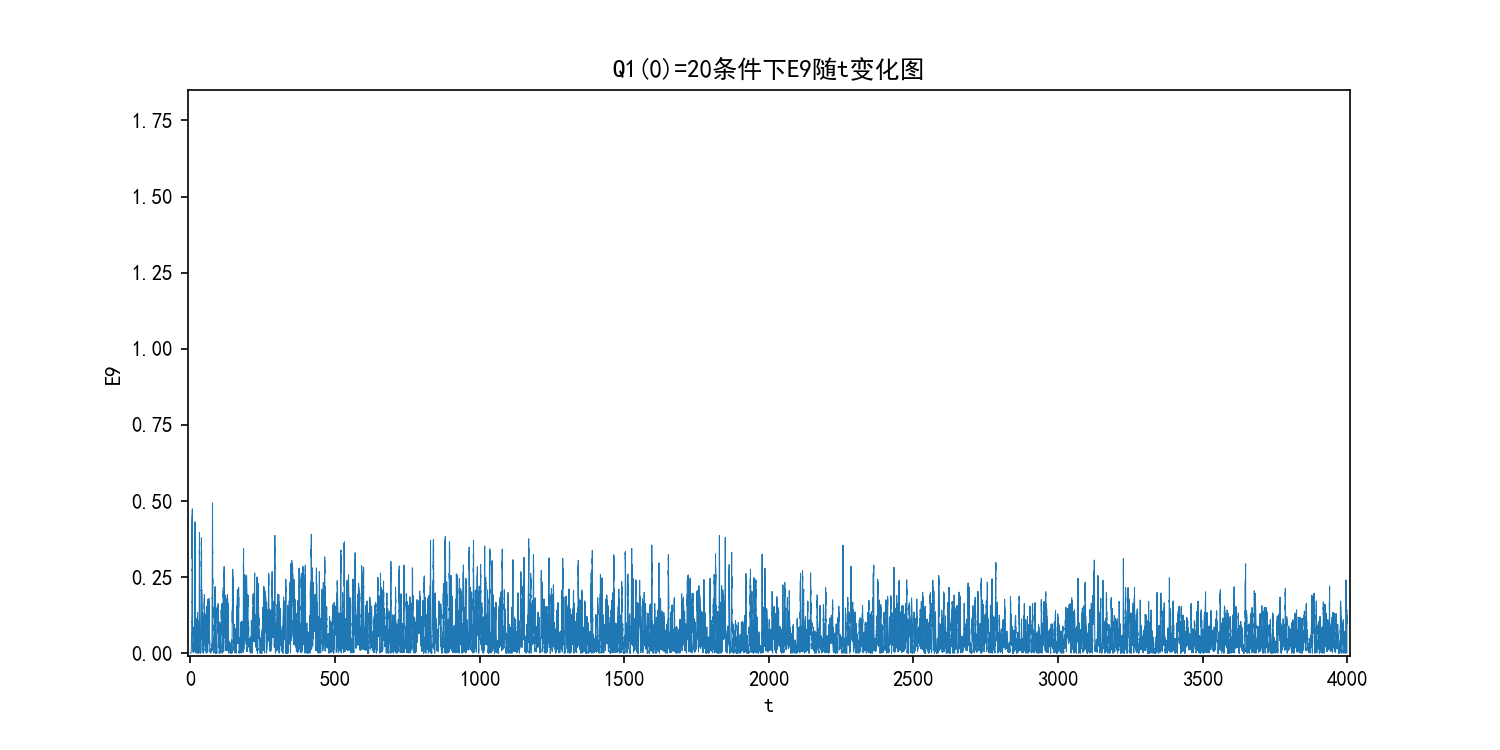
\includegraphics[width=\textwidth]{./q5_pics/exp/E9.png}
        \end{minipage}
        \caption{E9}\label{fig:E9 in q5}
    \end{figure}
    \begin{figure}[H]
        \begin{minipage}[t]{0.49\textwidth}
            \centering
            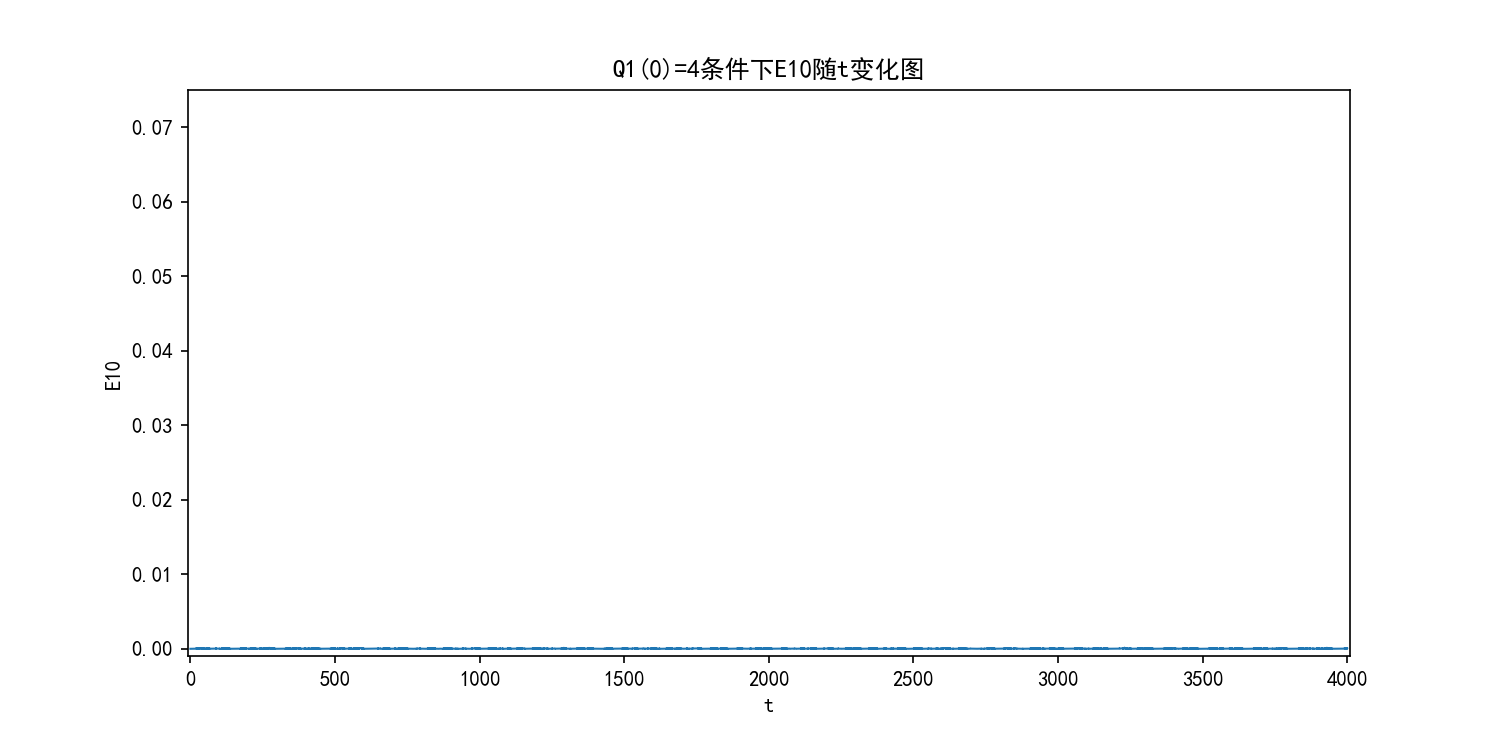
\includegraphics[width=\textwidth]{./q5_pics/cmp/E10.png}
        \end{minipage}
        \begin{minipage}[t]{0.49\textwidth}
            \centering
            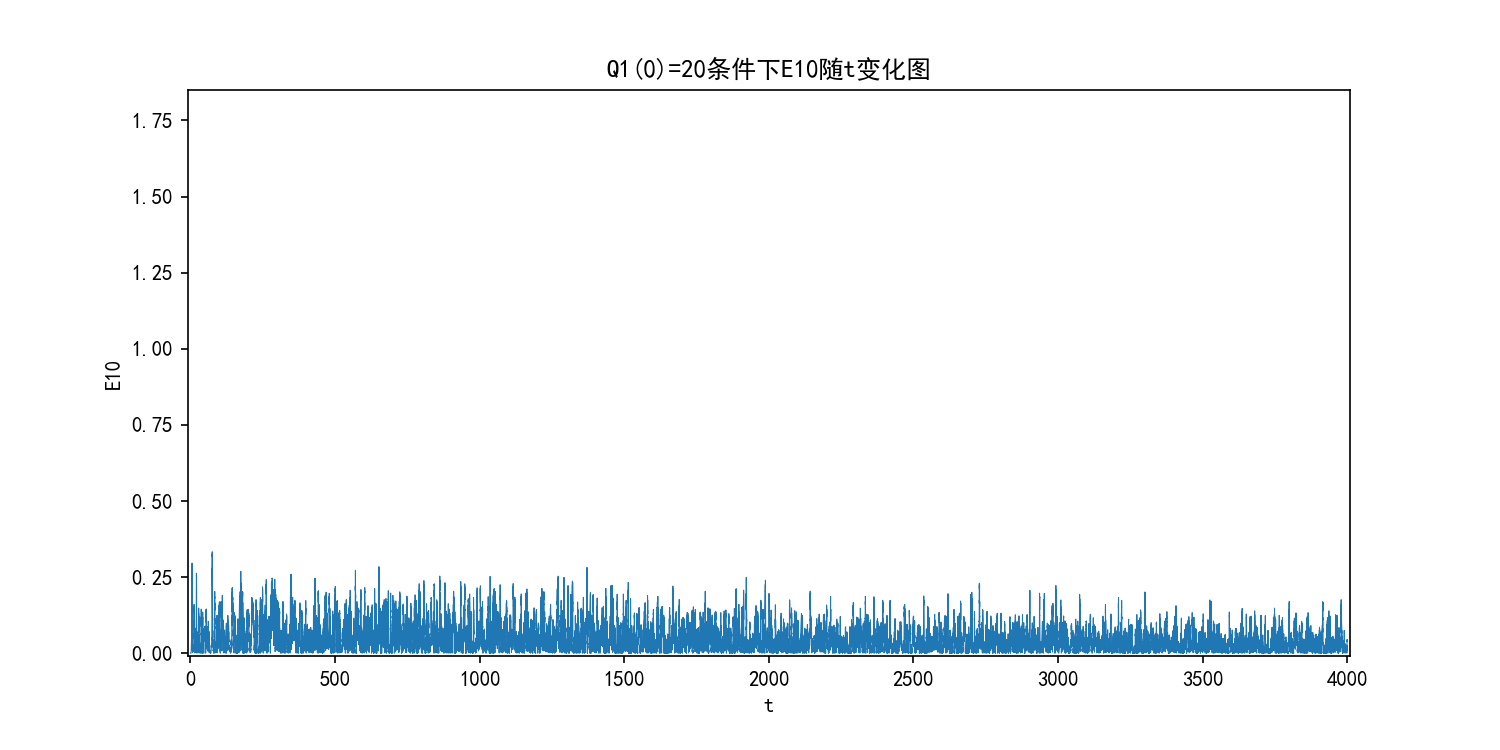
\includegraphics[width=\textwidth]{./q5_pics/exp/E10.png}
        \end{minipage}
        \caption{E10}\label{fig:E10 in q5}
    \end{figure}
    \begin{figure}[H]
        \begin{minipage}[t]{0.49\textwidth}
            \centering
            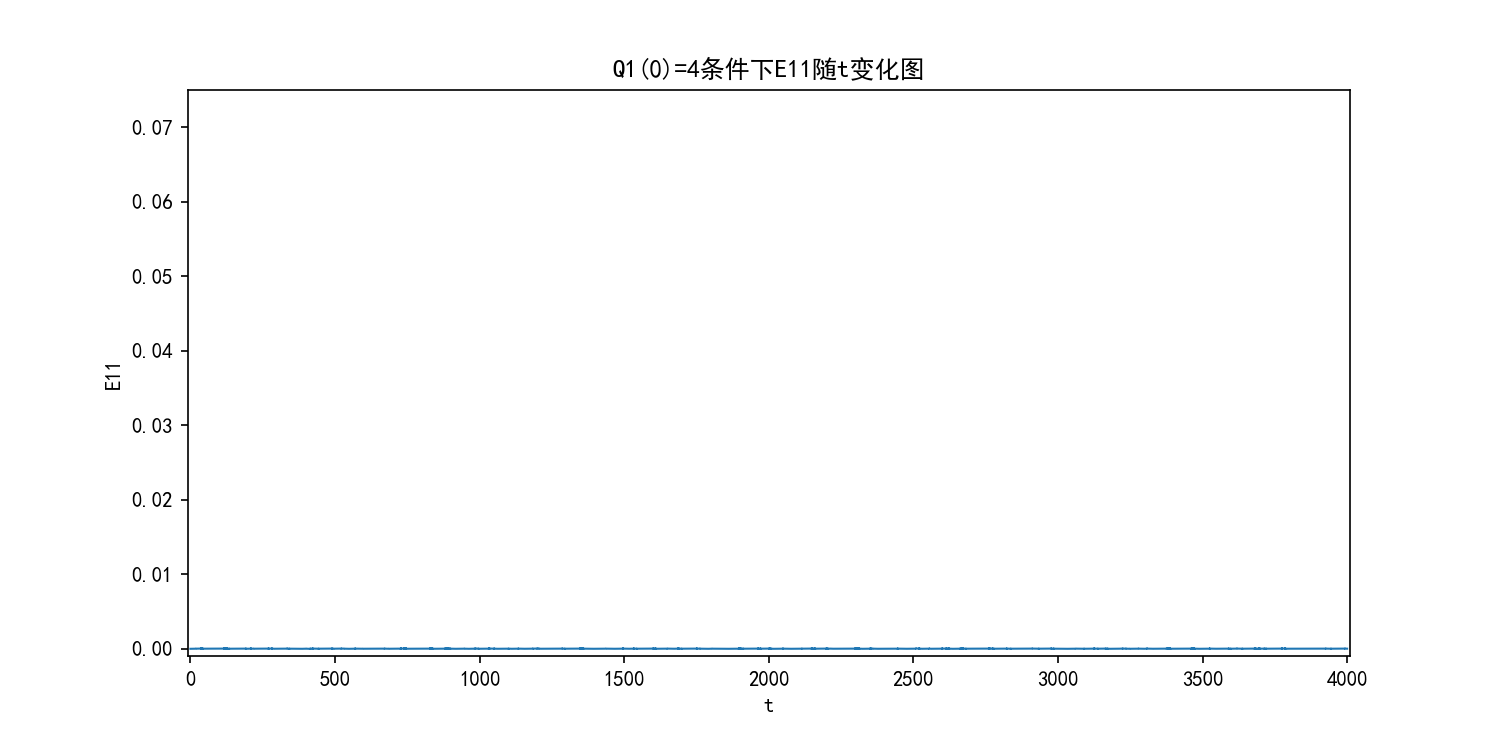
\includegraphics[width=\textwidth]{./q5_pics/cmp/E11.png}
        \end{minipage}
        \begin{minipage}[t]{0.49\textwidth}
            \centering
            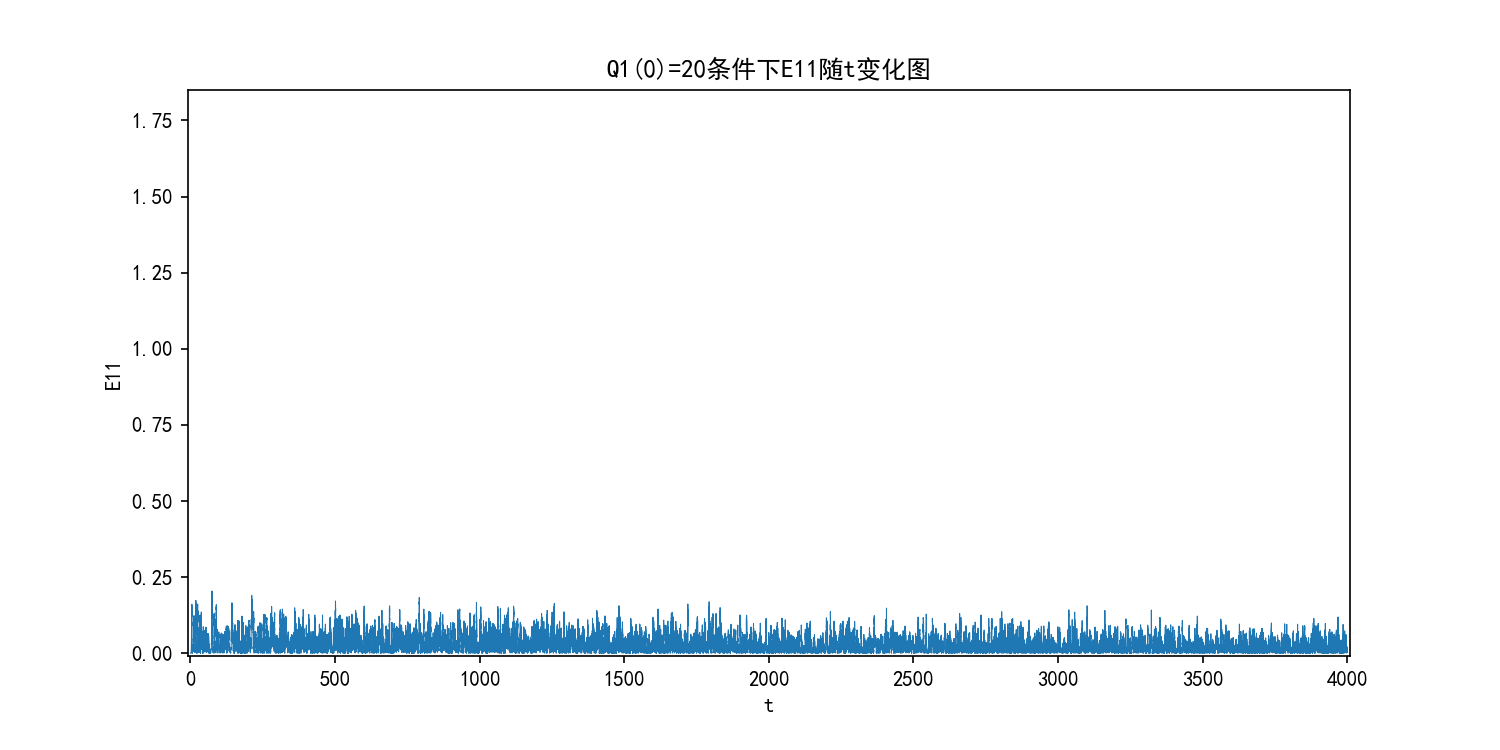
\includegraphics[width=\textwidth]{./q5_pics/exp/E11.png}
        \end{minipage}
        \caption{E11}\label{fig:E11 in q5}
    \end{figure}
    \begin{figure}[H]
        \begin{minipage}[t]{0.49\textwidth}
            \centering
            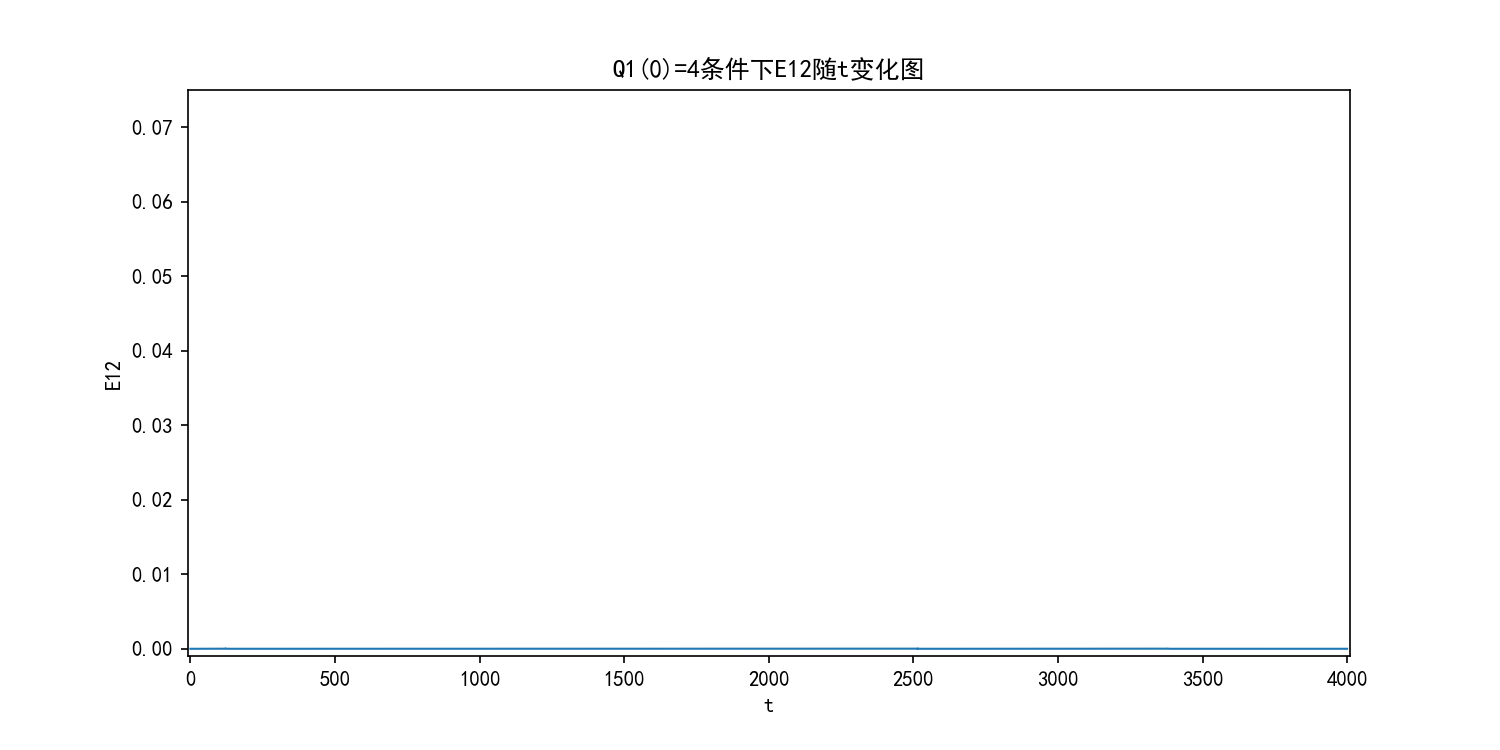
\includegraphics[width=\textwidth]{./q5_pics/cmp/E12.png}
        \end{minipage}
        \begin{minipage}[t]{0.49\textwidth}
            \centering
            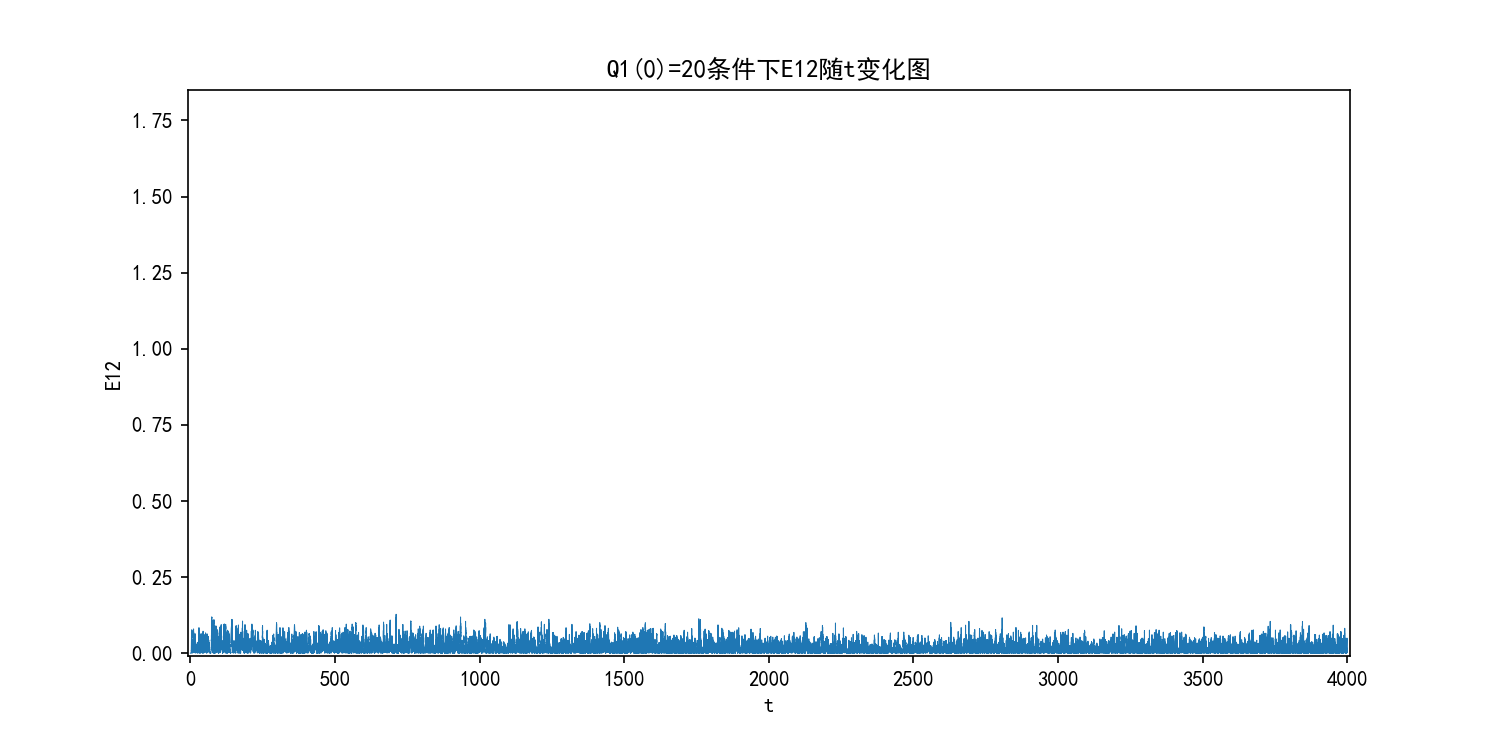
\includegraphics[width=\textwidth]{./q5_pics/exp/E12.png}
        \end{minipage}
        \caption{E12}\label{fig:E12 in q5}
    \end{figure}
    \begin{figure}[H]
        \begin{minipage}[t]{0.49\textwidth}
            \centering
            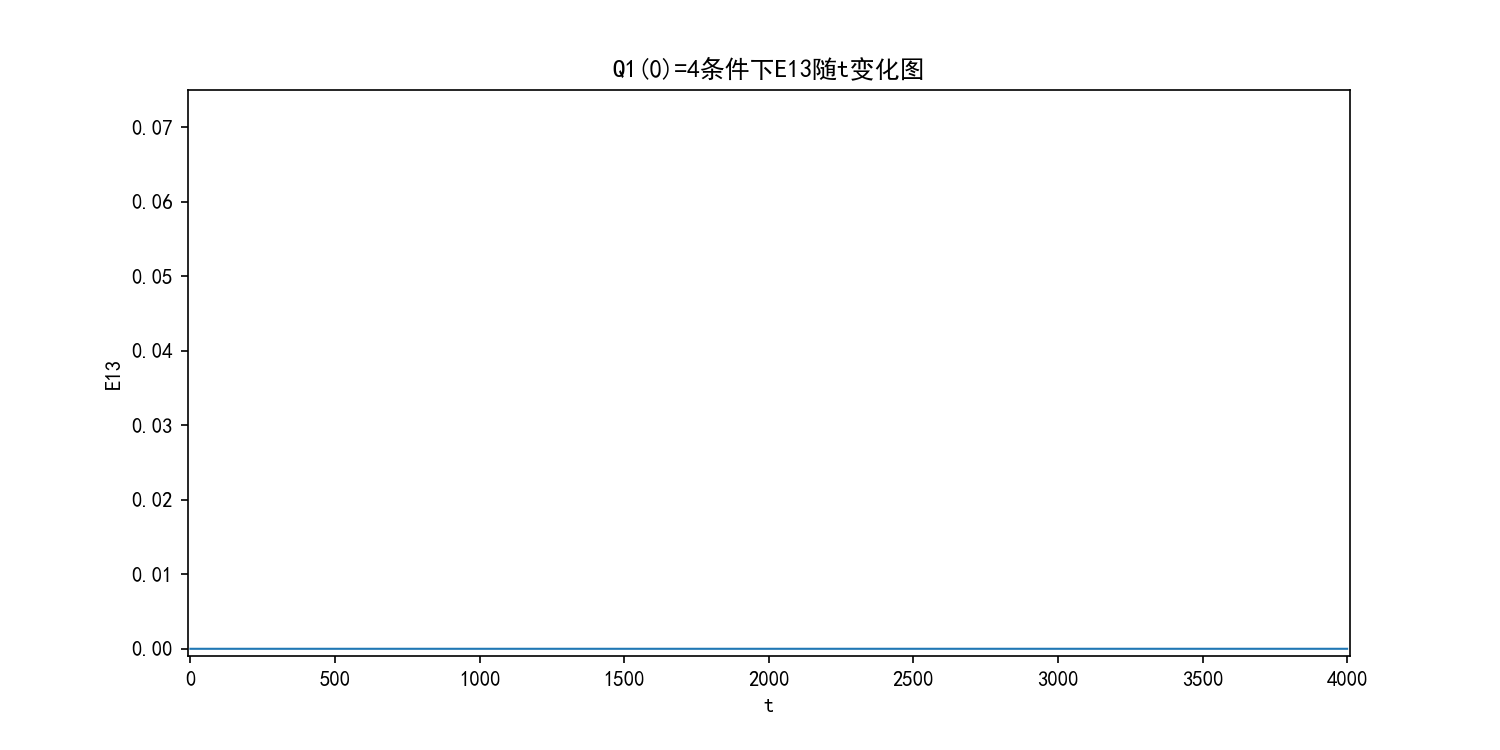
\includegraphics[width=\textwidth]{./q5_pics/cmp/E13.png}
        \end{minipage}
        \begin{minipage}[t]{0.49\textwidth}
            \centering
            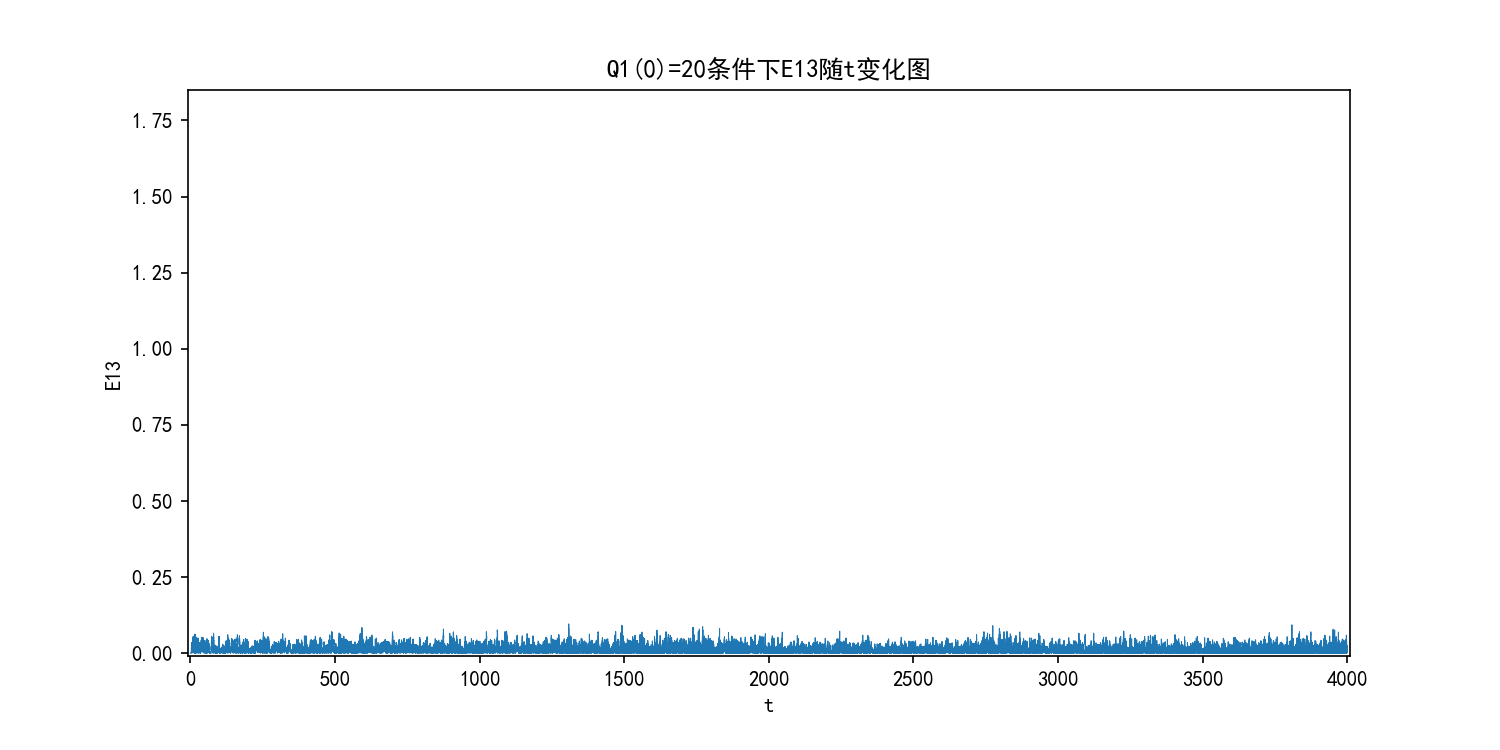
\includegraphics[width=\textwidth]{./q5_pics/exp/E13.png}
        \end{minipage}
        \caption{E13}\label{fig:E13 in q5}
    \end{figure}
    \begin{figure}[H]
        \begin{minipage}[t]{0.49\textwidth}
            \centering
            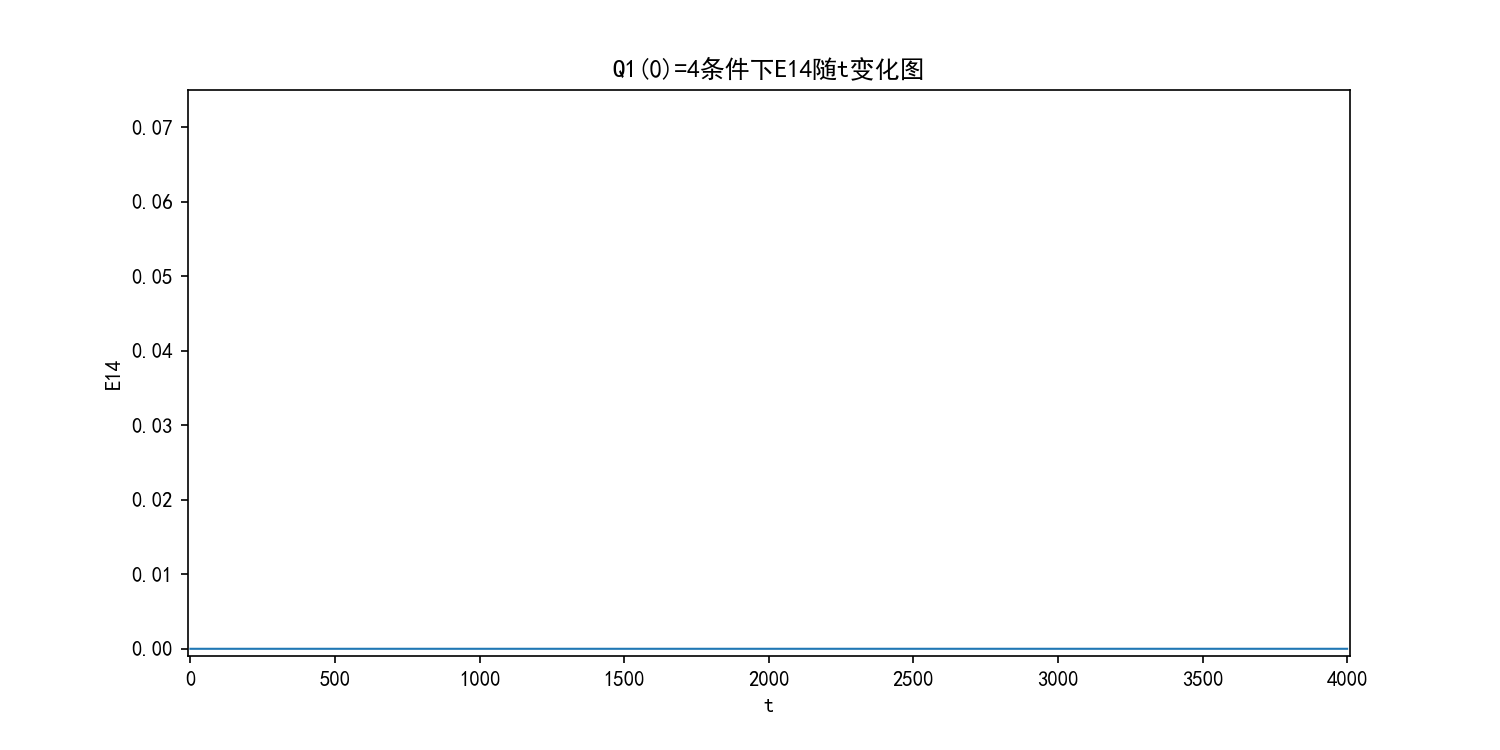
\includegraphics[width=\textwidth]{./q5_pics/cmp/E14.png}
        \end{minipage}
        \begin{minipage}[t]{0.49\textwidth}
            \centering
            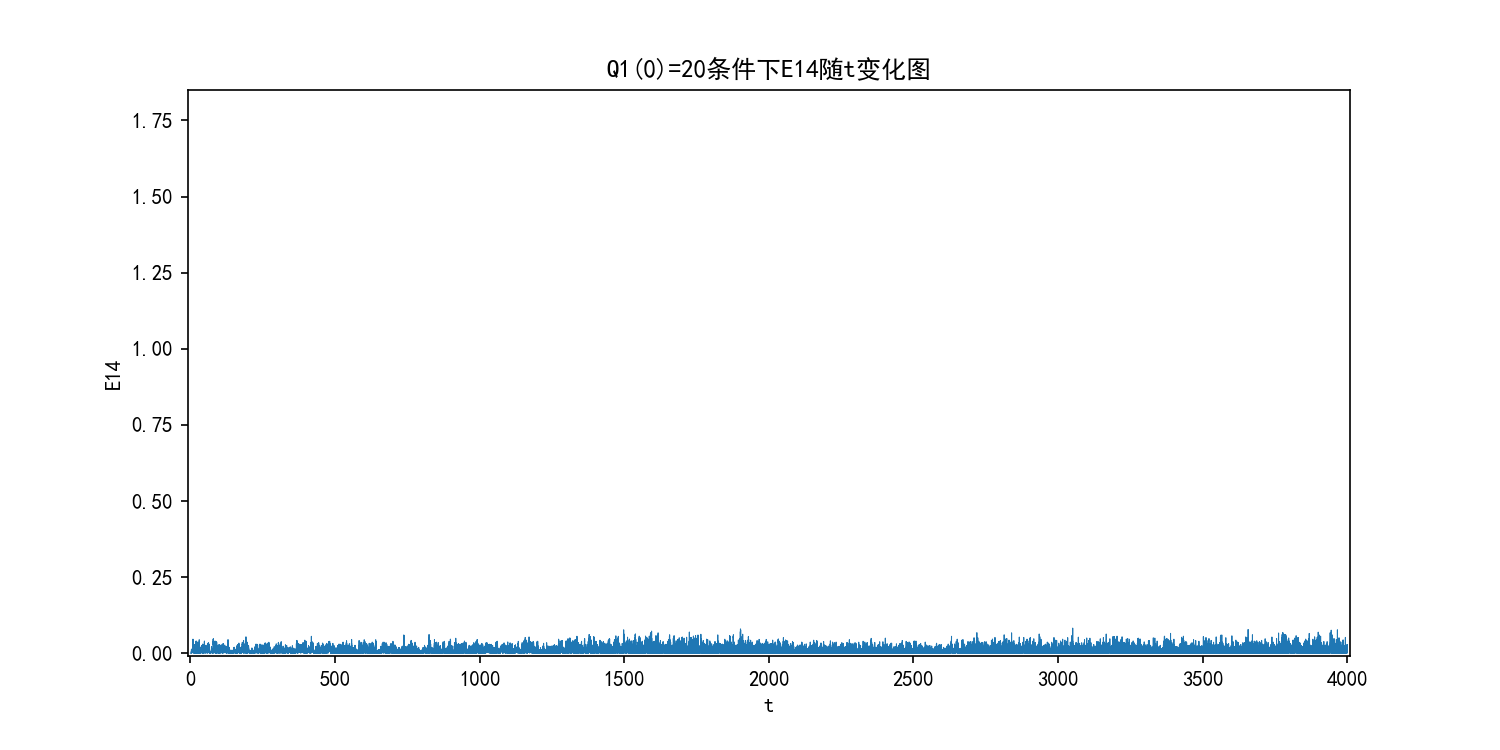
\includegraphics[width=\textwidth]{./q5_pics/exp/E14.png}
        \end{minipage}
        \caption{E14}\label{fig:E14 in q5}
    \end{figure}
    \begin{figure}[H]
        \begin{minipage}[t]{0.49\textwidth}
            \centering
            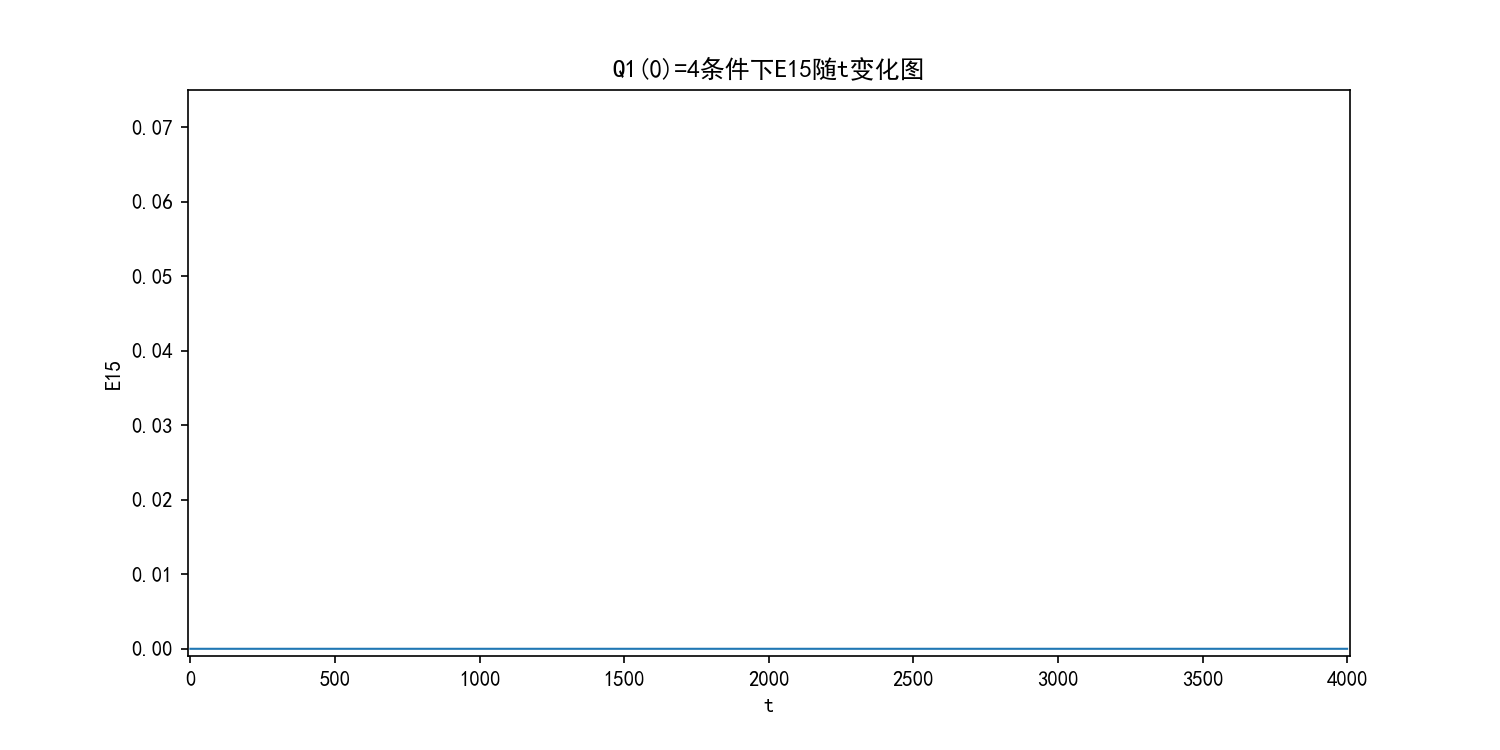
\includegraphics[width=\textwidth]{./q5_pics/cmp/E15.png}
        \end{minipage}
        \begin{minipage}[t]{0.49\textwidth}
            \centering
            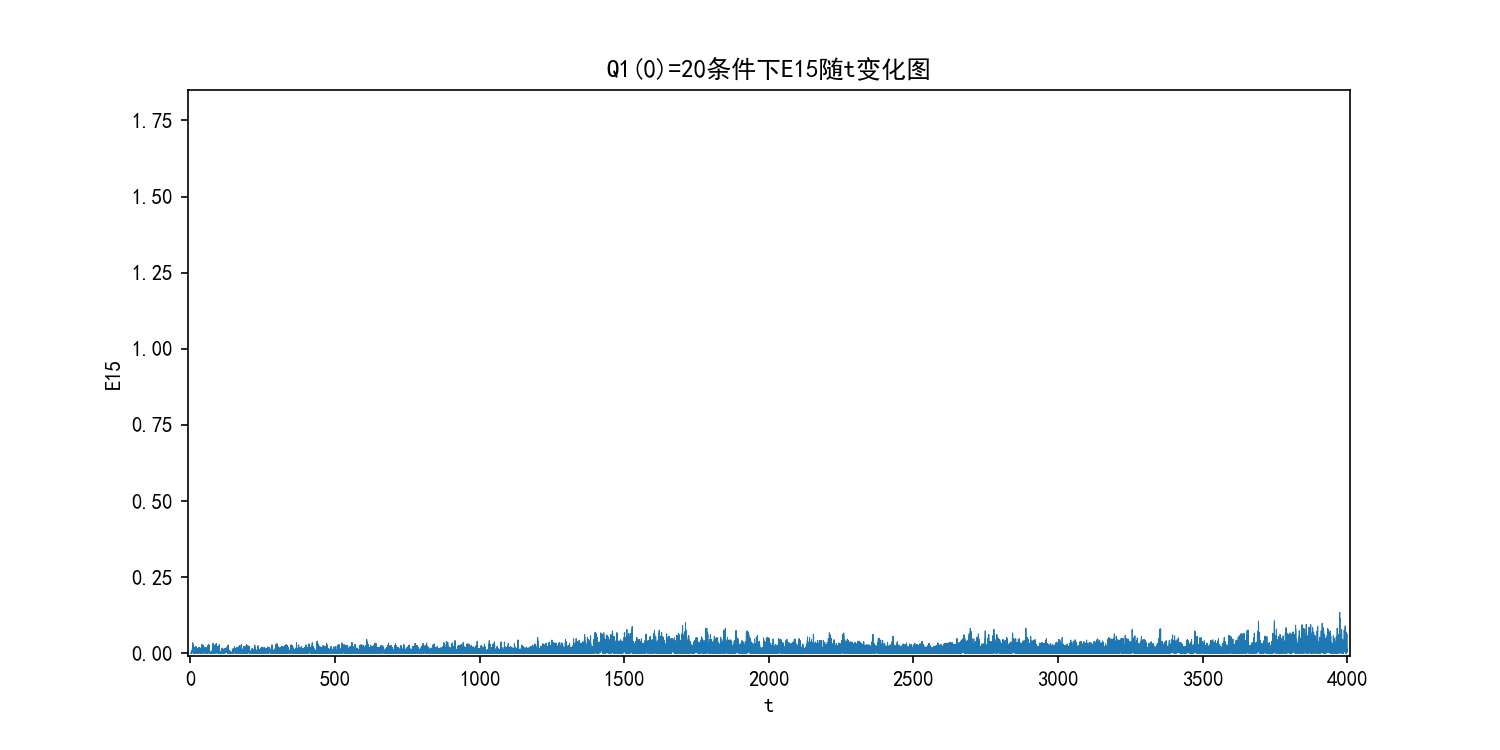
\includegraphics[width=\textwidth]{./q5_pics/exp/E15.png}
        \end{minipage}
        \caption{E15}\label{fig:E15 in q5}
    \end{figure}
    \begin{figure}[H]
        \begin{minipage}[t]{0.49\textwidth}
            \centering
            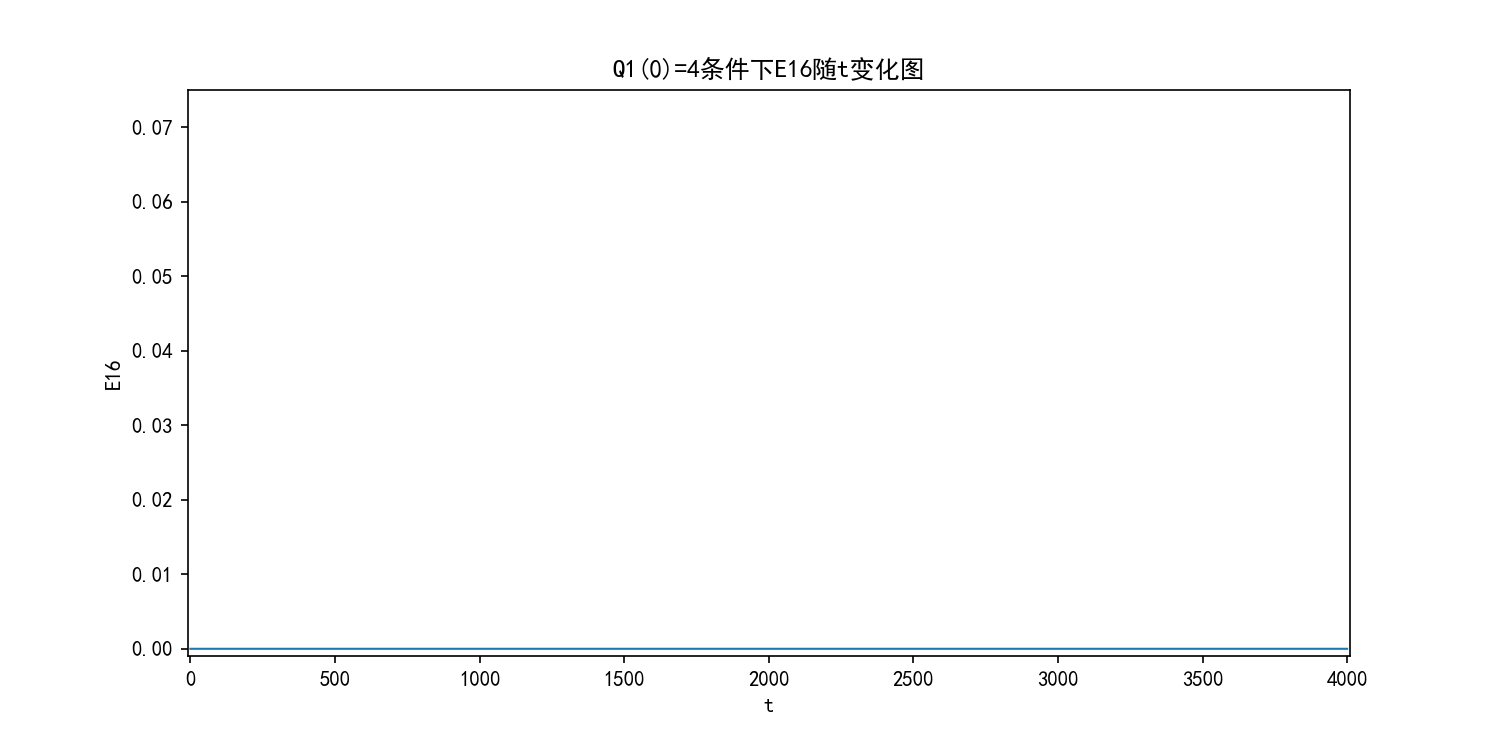
\includegraphics[width=\textwidth]{./q5_pics/cmp/E16.png}
        \end{minipage}
        \begin{minipage}[t]{0.49\textwidth}
            \centering
            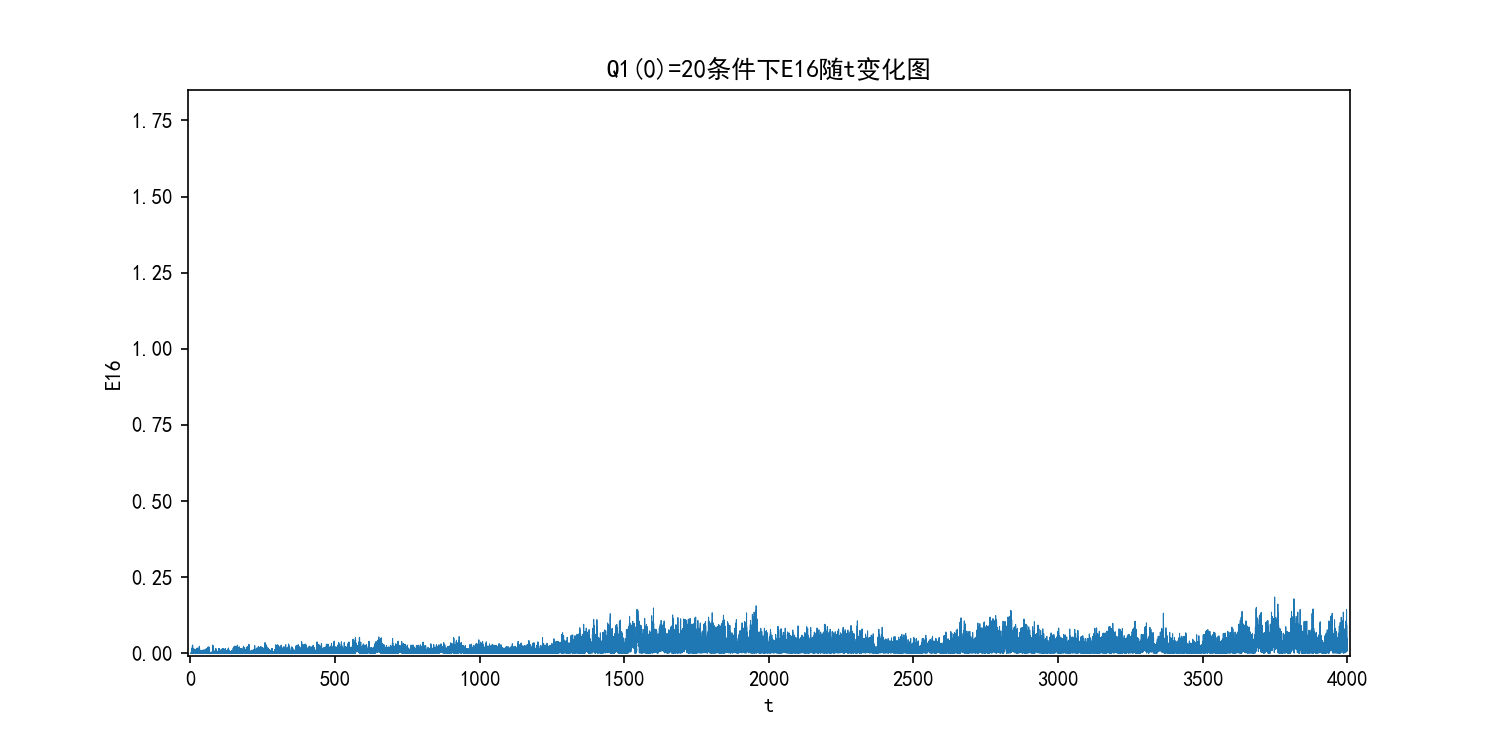
\includegraphics[width=\textwidth]{./q5_pics/exp/E16.png}
        \end{minipage}
        \caption{E16}\label{fig:E16 in q5}
    \end{figure}
    \begin{figure}[H]
        \begin{minipage}[t]{0.49\textwidth}
            \centering
            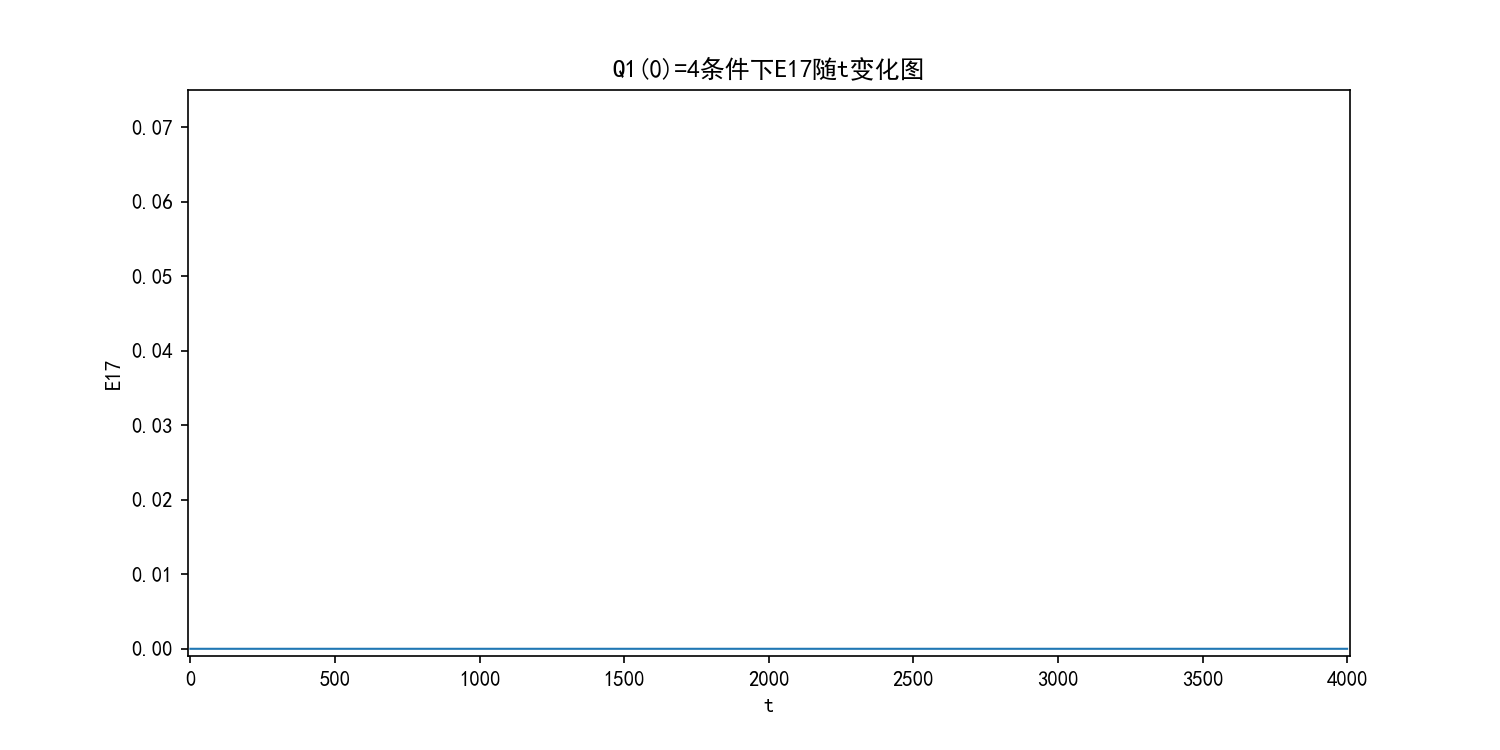
\includegraphics[width=\textwidth]{./q5_pics/cmp/E17.png}
        \end{minipage}
        \begin{minipage}[t]{0.49\textwidth}
            \centering
            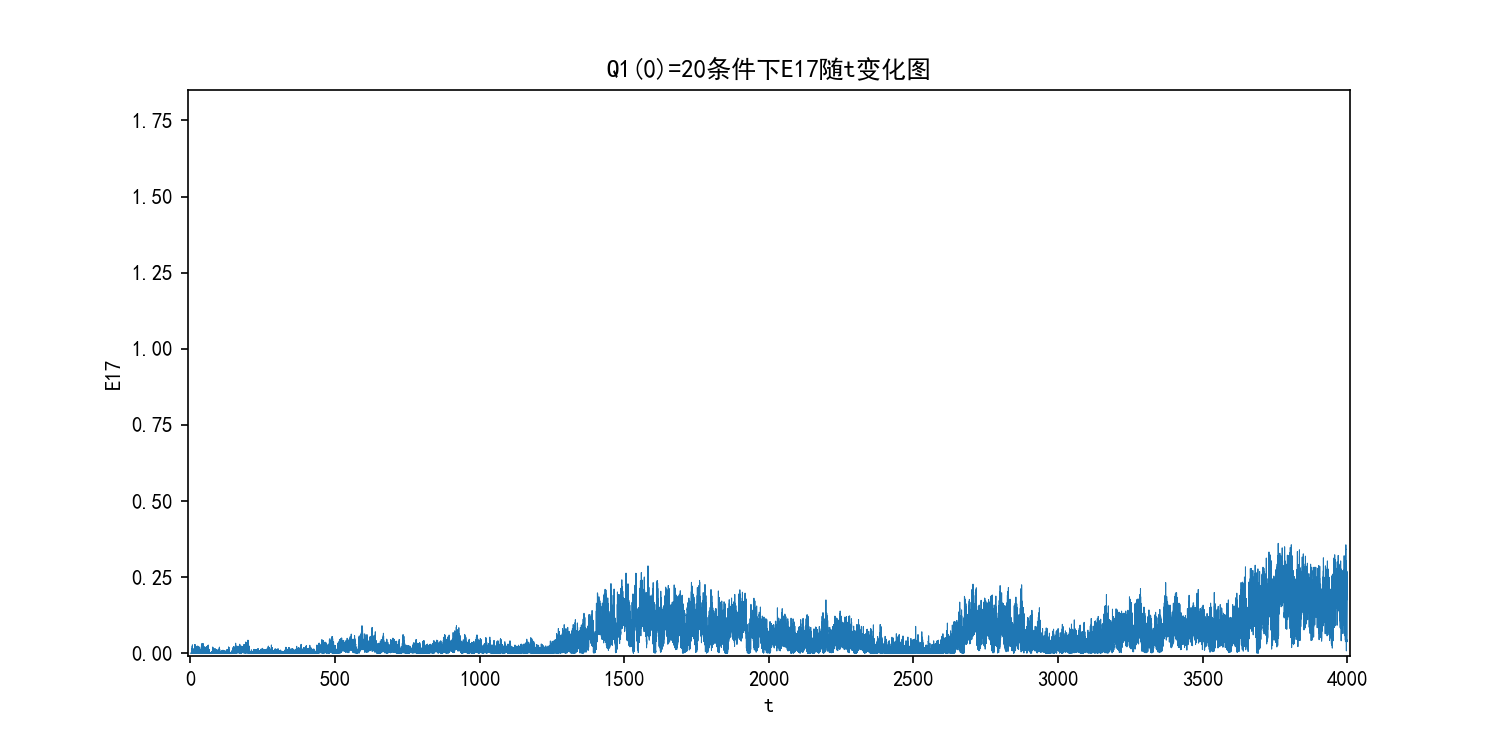
\includegraphics[width=\textwidth]{./q5_pics/exp/E17.png}
        \end{minipage}
        \caption{E17}\label{fig:E17 in q5}
    \end{figure}
    \begin{figure}[H]
        \begin{minipage}[t]{0.49\textwidth}
            \centering
            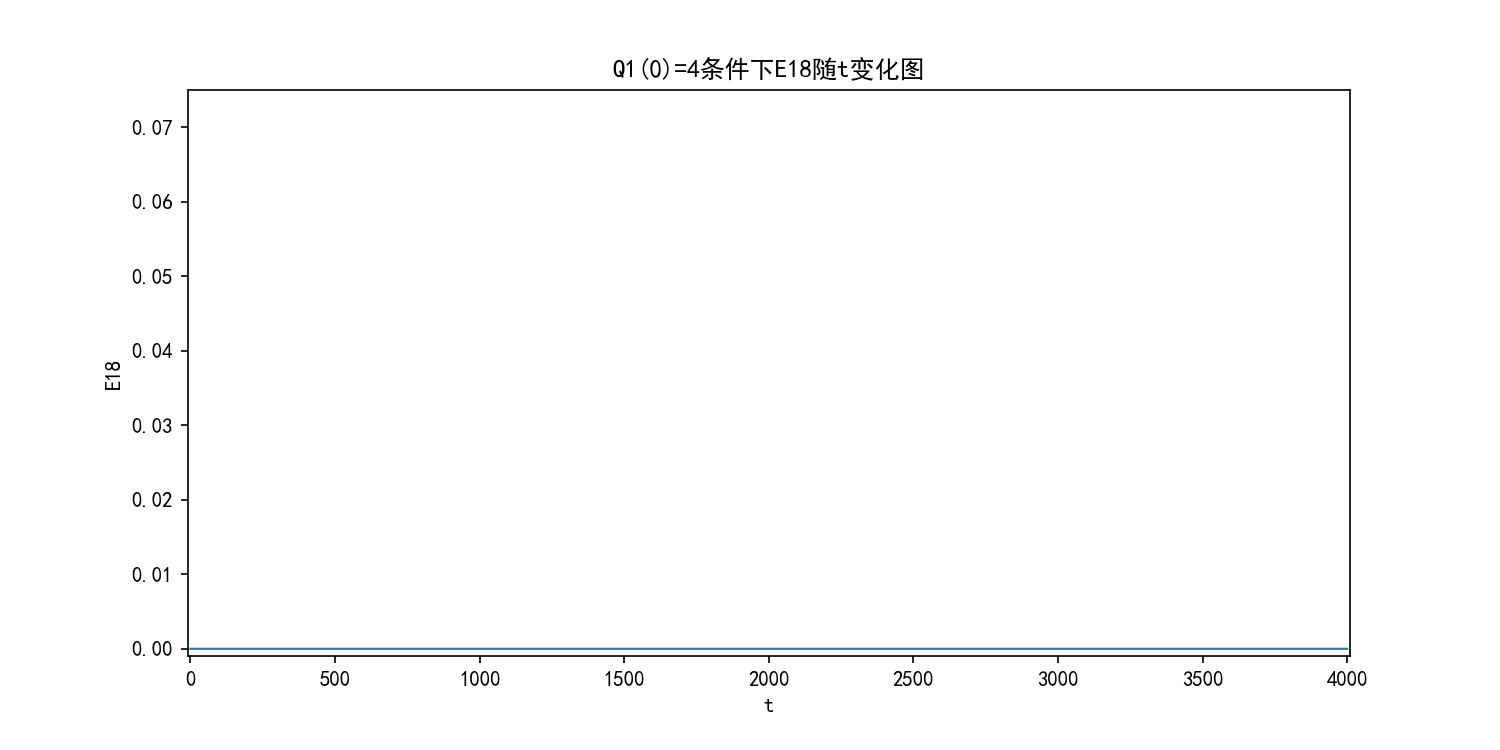
\includegraphics[width=\textwidth]{./q5_pics/cmp/E18.png}
        \end{minipage}
        \begin{minipage}[t]{0.49\textwidth}
            \centering
            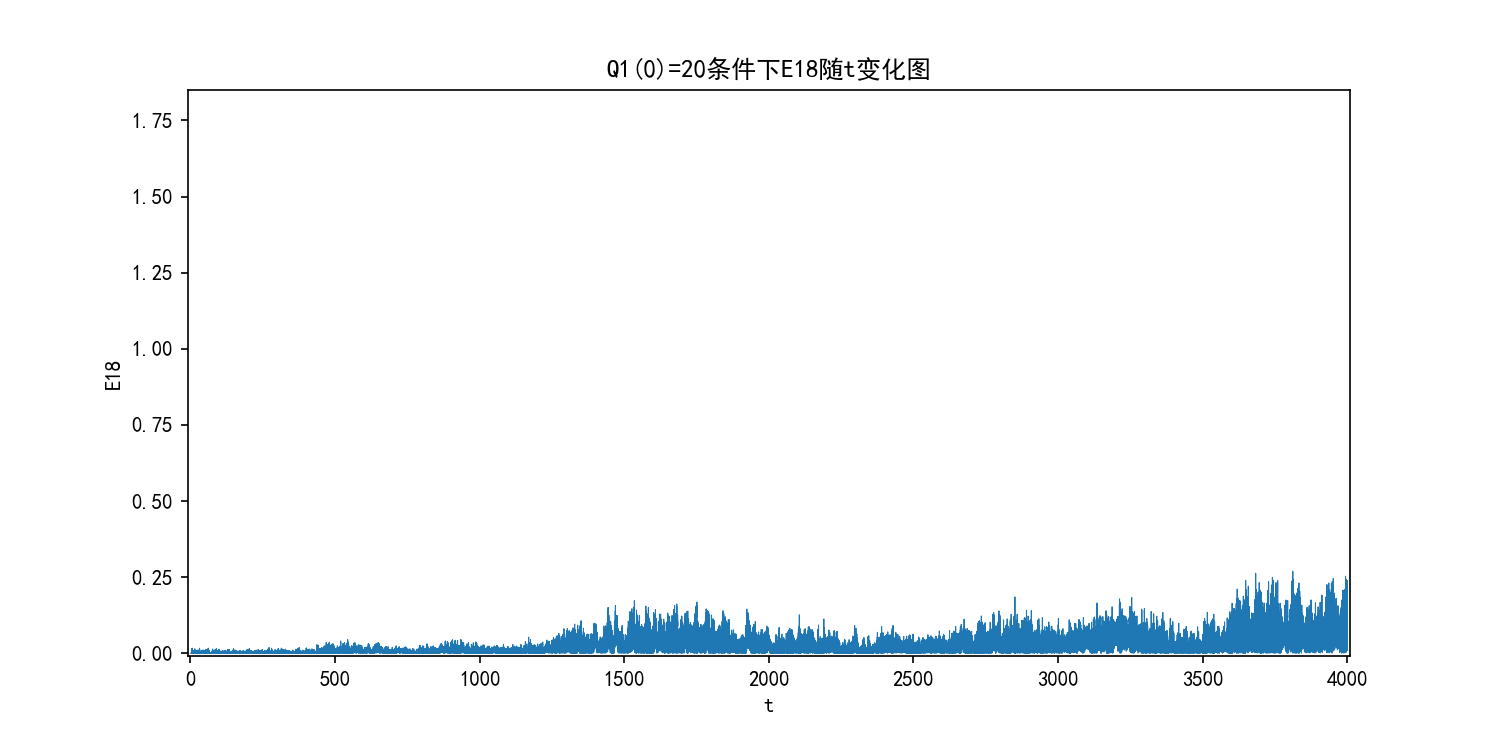
\includegraphics[width=\textwidth]{./q5_pics/exp/E18.png}
        \end{minipage}
        \caption{E18}\label{fig:E18 in q5}
    \end{figure}
    \begin{figure}[H]
        \begin{minipage}[t]{0.49\textwidth}
            \centering
            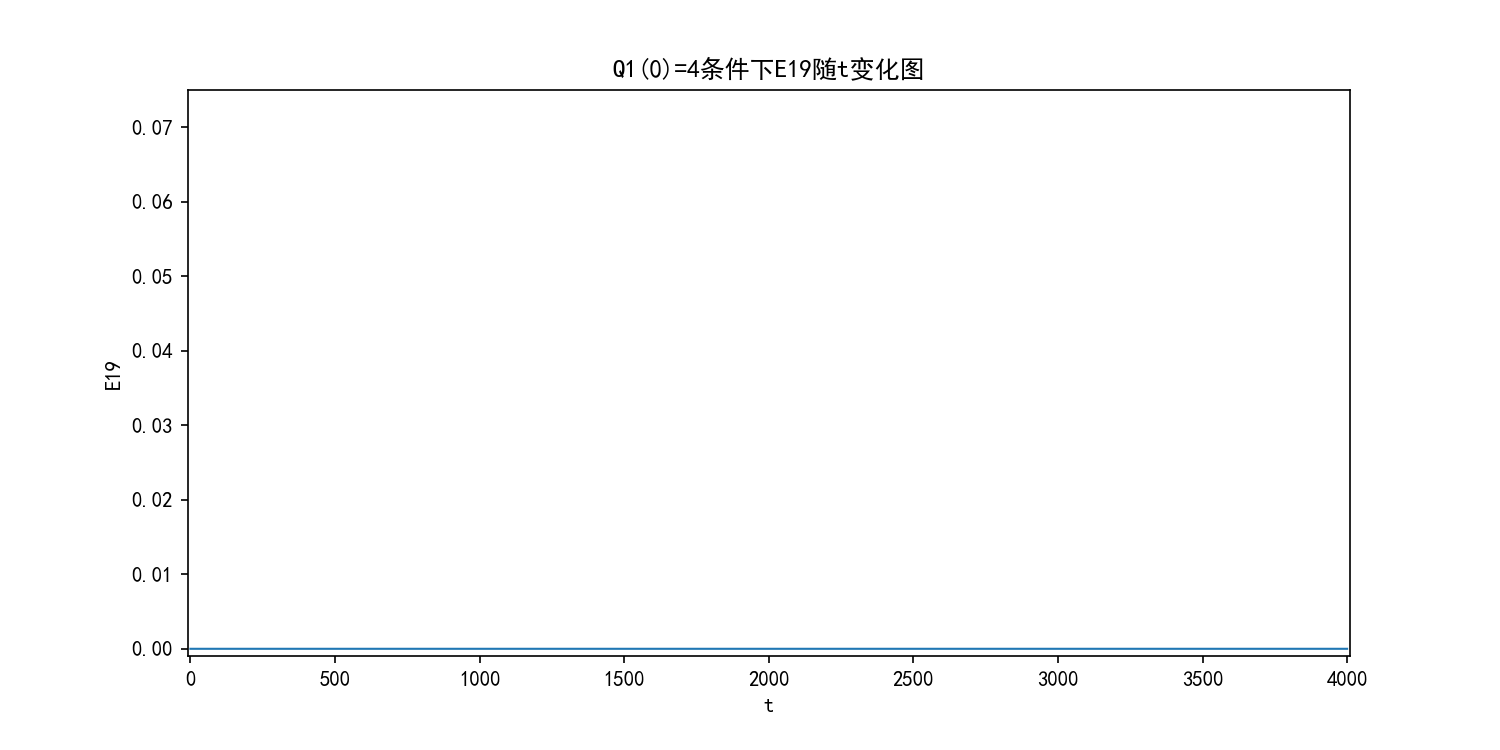
\includegraphics[width=\textwidth]{./q5_pics/cmp/E19.png}
        \end{minipage}
        \begin{minipage}[t]{0.49\textwidth}
            \centering
            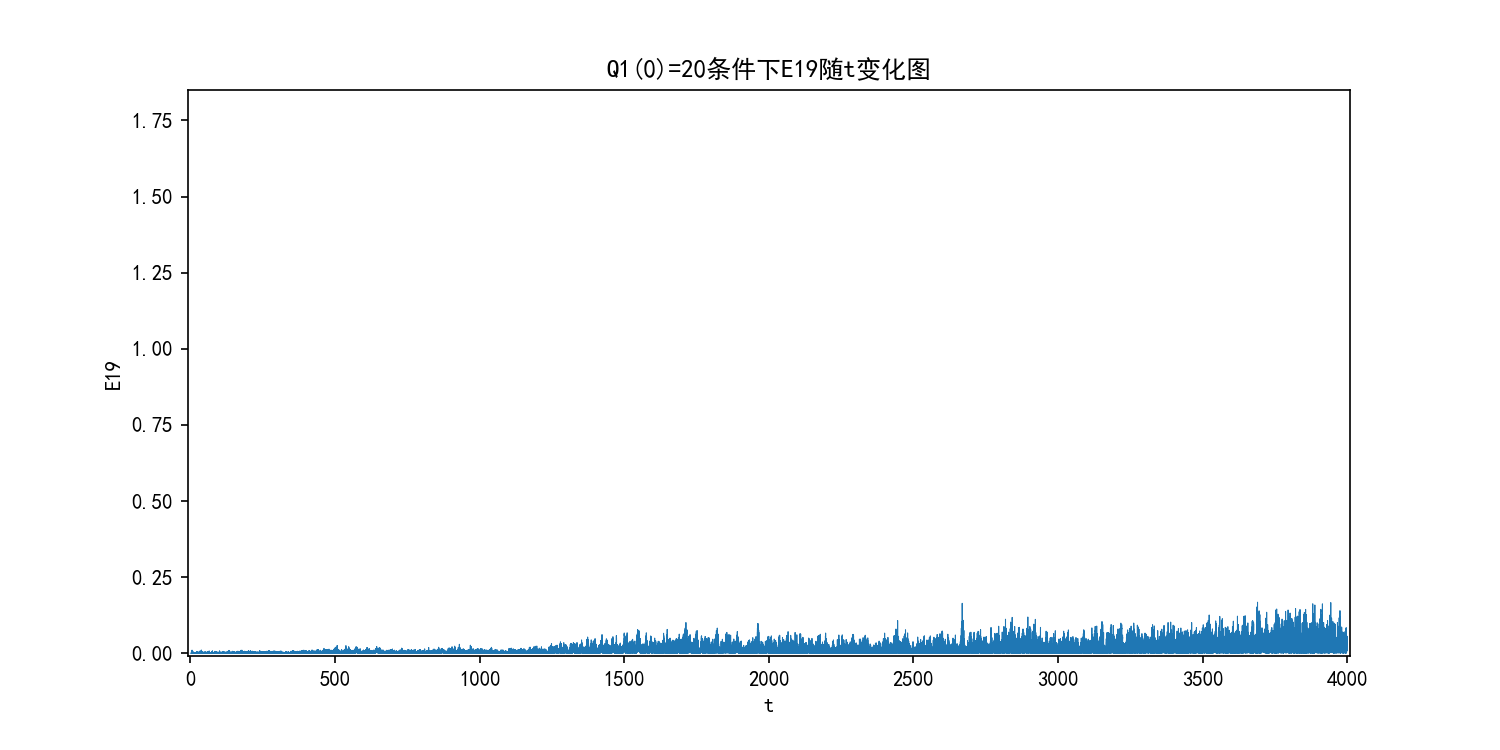
\includegraphics[width=\textwidth]{./q5_pics/exp/E19.png}
        \end{minipage}
        \caption{E19}\label{fig:E19 in q5}
    \end{figure}
    \begin{figure}[H]
        \begin{minipage}[t]{0.49\textwidth}
            \centering
            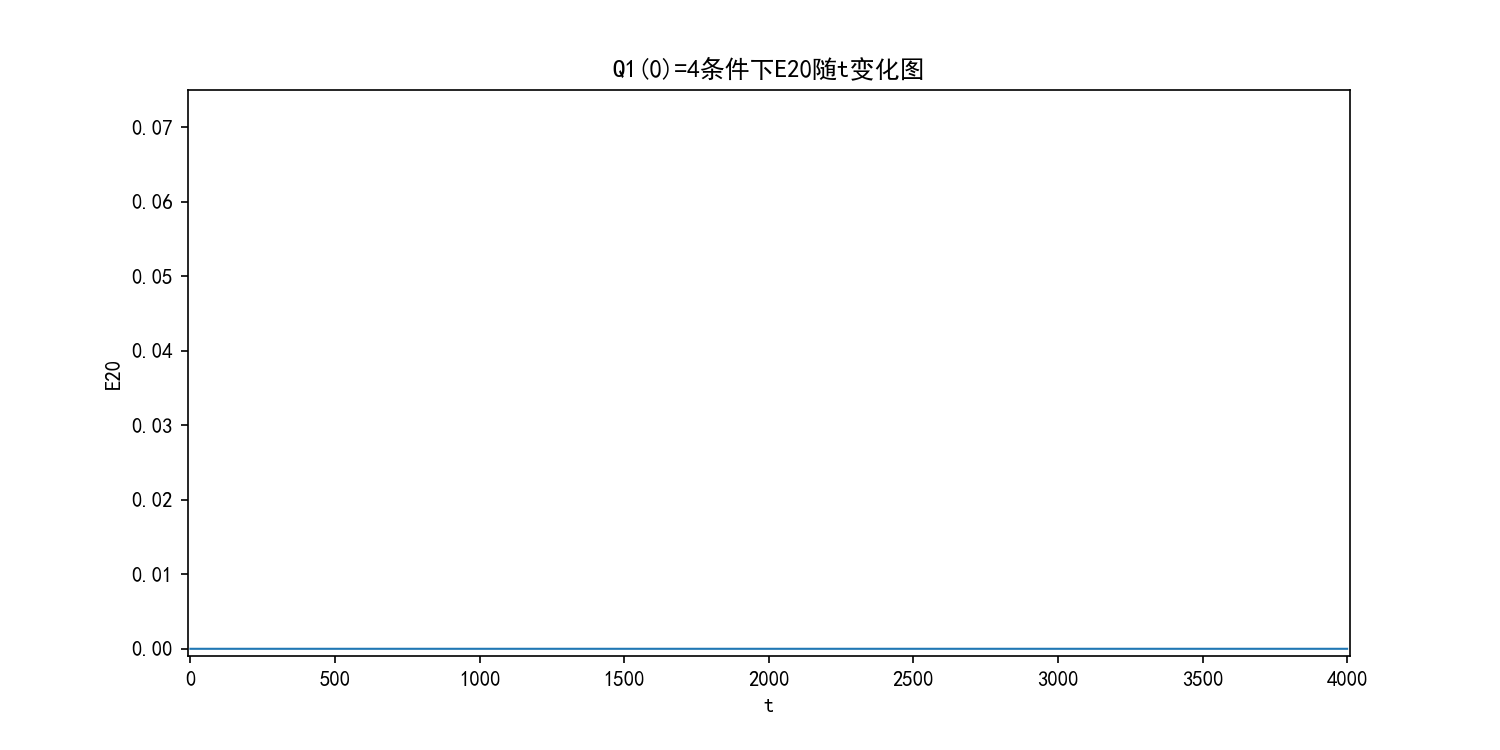
\includegraphics[width=\textwidth]{./q5_pics/cmp/E20.png}
        \end{minipage}
        \begin{minipage}[t]{0.49\textwidth}
            \centering
            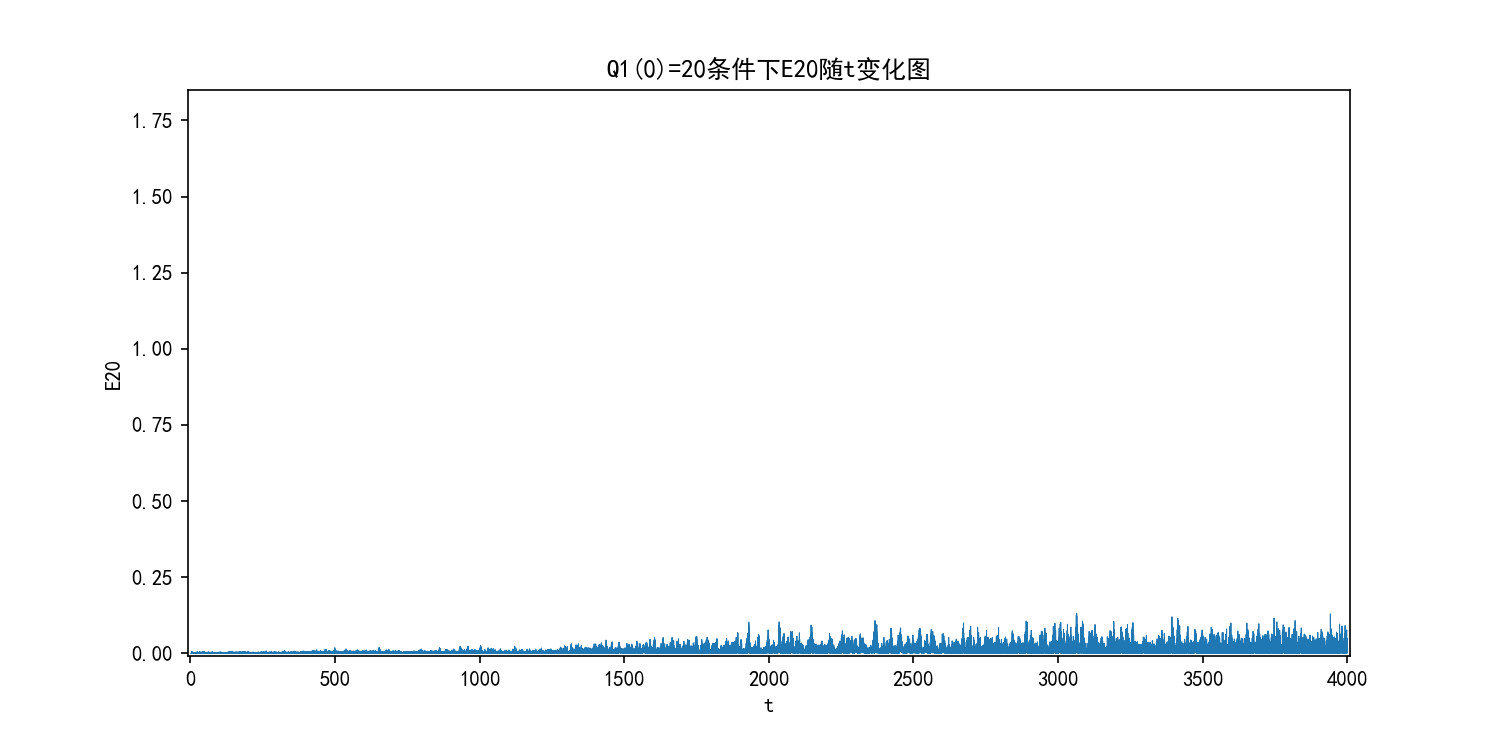
\includegraphics[width=\textwidth]{./q5_pics/exp/E20.png}
        \end{minipage}
        \caption{E20}\label{fig:E20 in q5}
    \end{figure}
    \begin{figure}[H]
        \begin{minipage}[t]{0.49\textwidth}
            \centering
            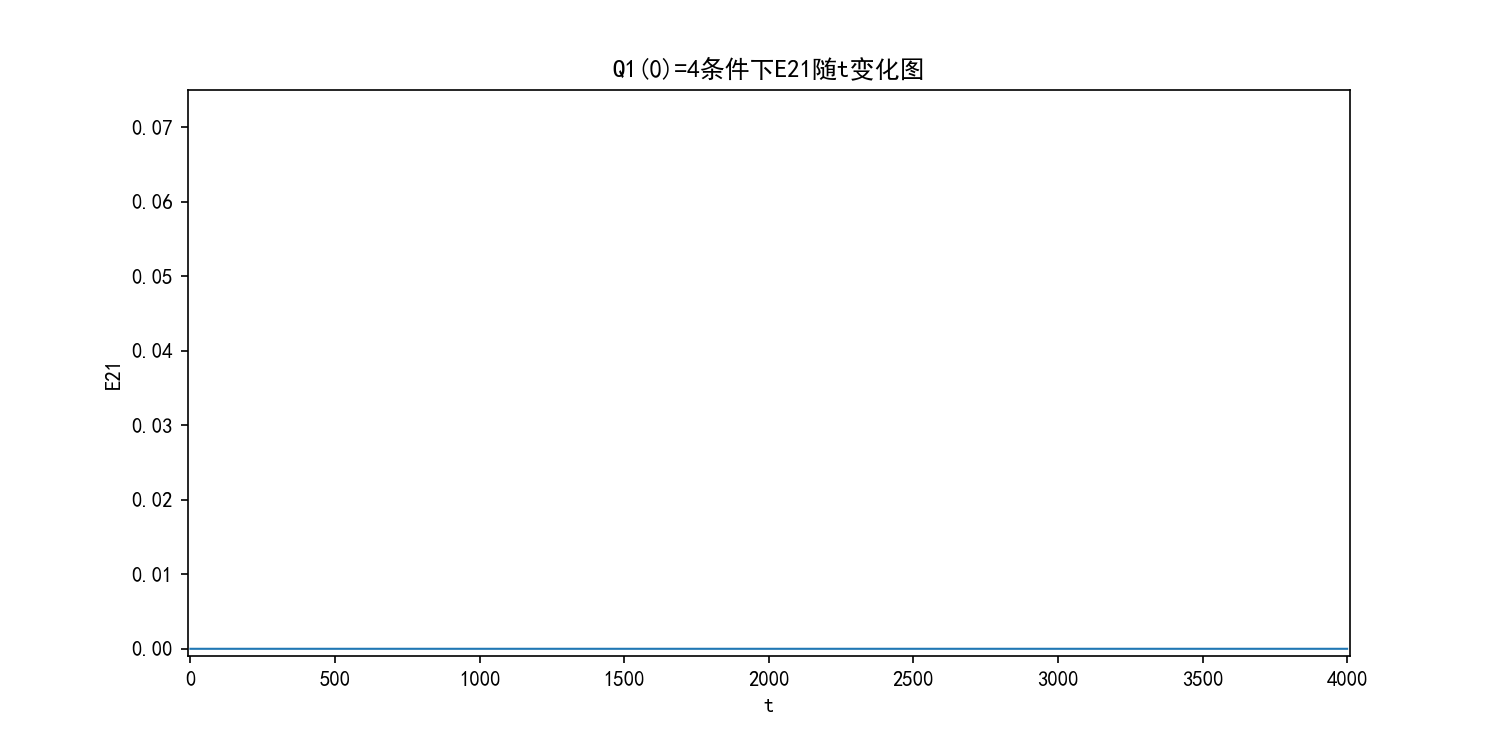
\includegraphics[width=\textwidth]{./q5_pics/cmp/E21.png}
        \end{minipage}
        \begin{minipage}[t]{0.49\textwidth}
            \centering
            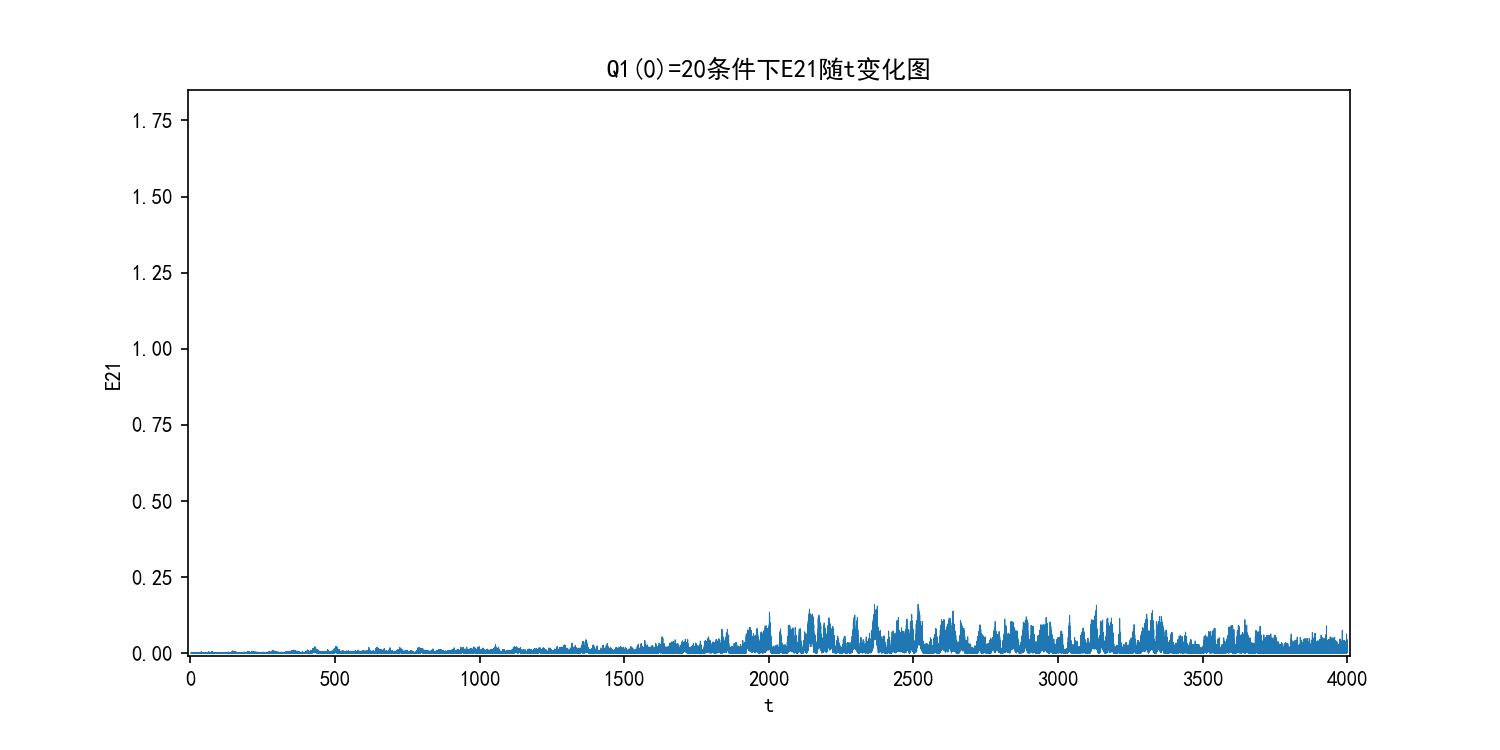
\includegraphics[width=\textwidth]{./q5_pics/exp/E21.png}
        \end{minipage}
        \caption{E21}\label{fig:E21 in q5}
    \end{figure}
    \begin{figure}[H]
        \begin{minipage}[t]{0.49\textwidth}
            \centering
            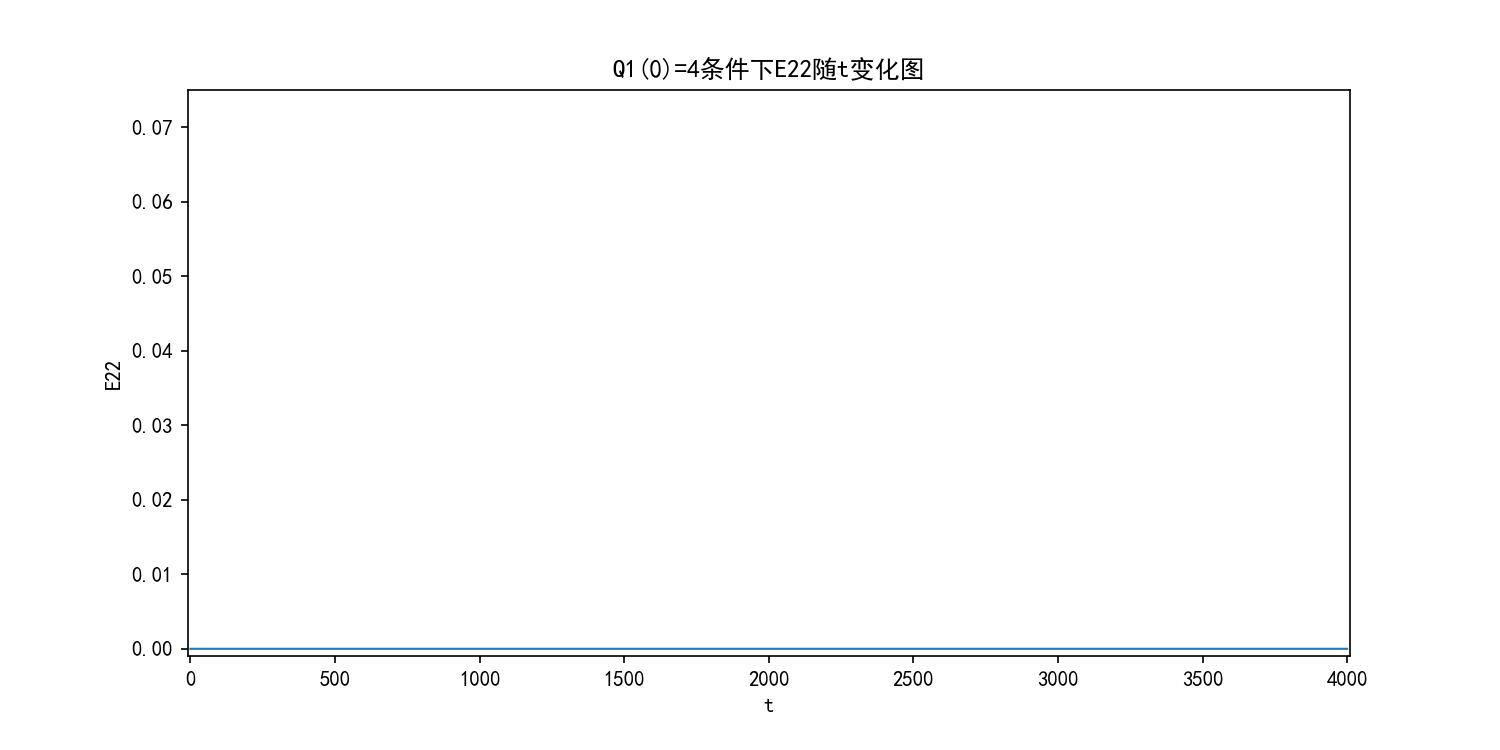
\includegraphics[width=\textwidth]{./q5_pics/cmp/E22.png}
        \end{minipage}
        \begin{minipage}[t]{0.49\textwidth}
            \centering
            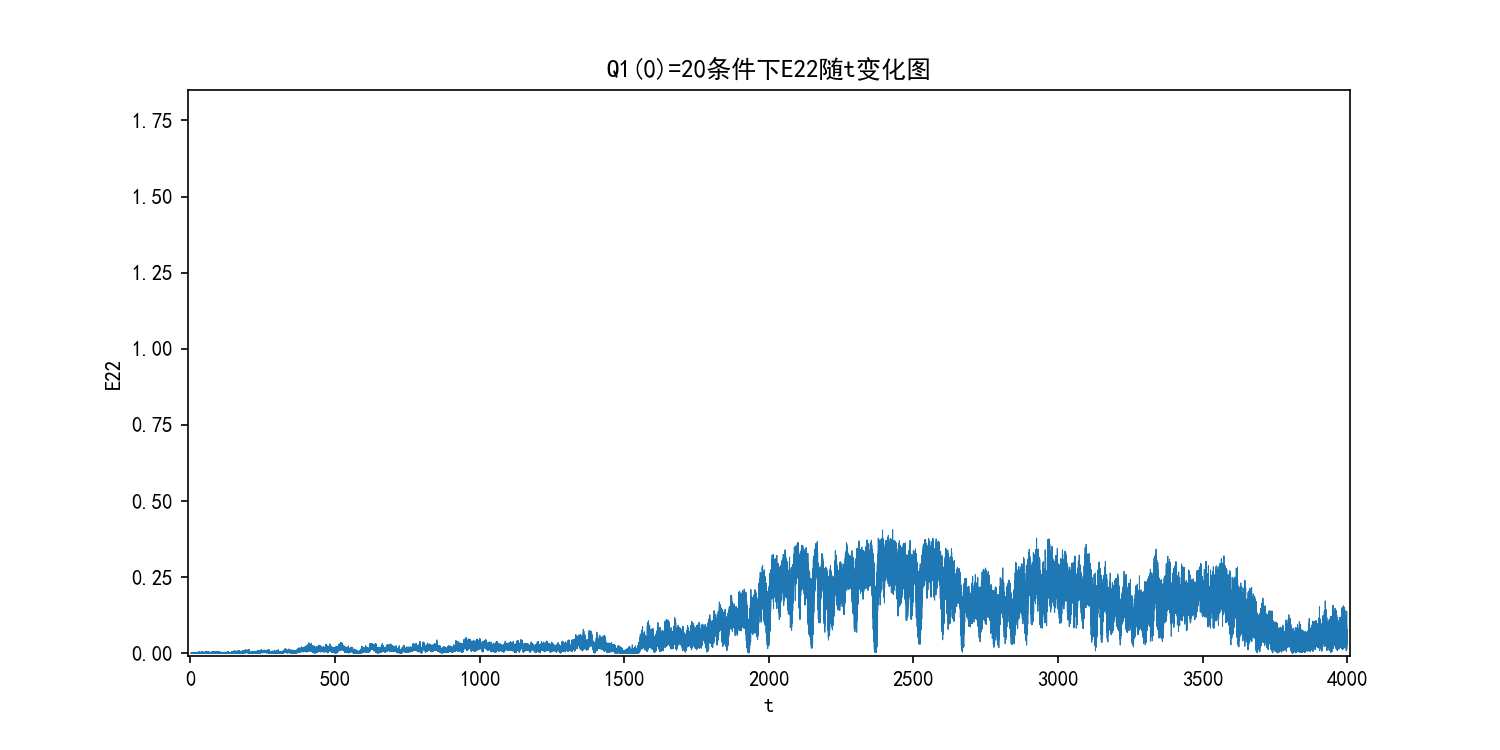
\includegraphics[width=\textwidth]{./q5_pics/exp/E22.png}
        \end{minipage}
        \caption{E22}\label{fig:E22 in q5}
    \end{figure}
    \begin{figure}[H]
        \begin{minipage}[t]{0.49\textwidth}
            \centering
            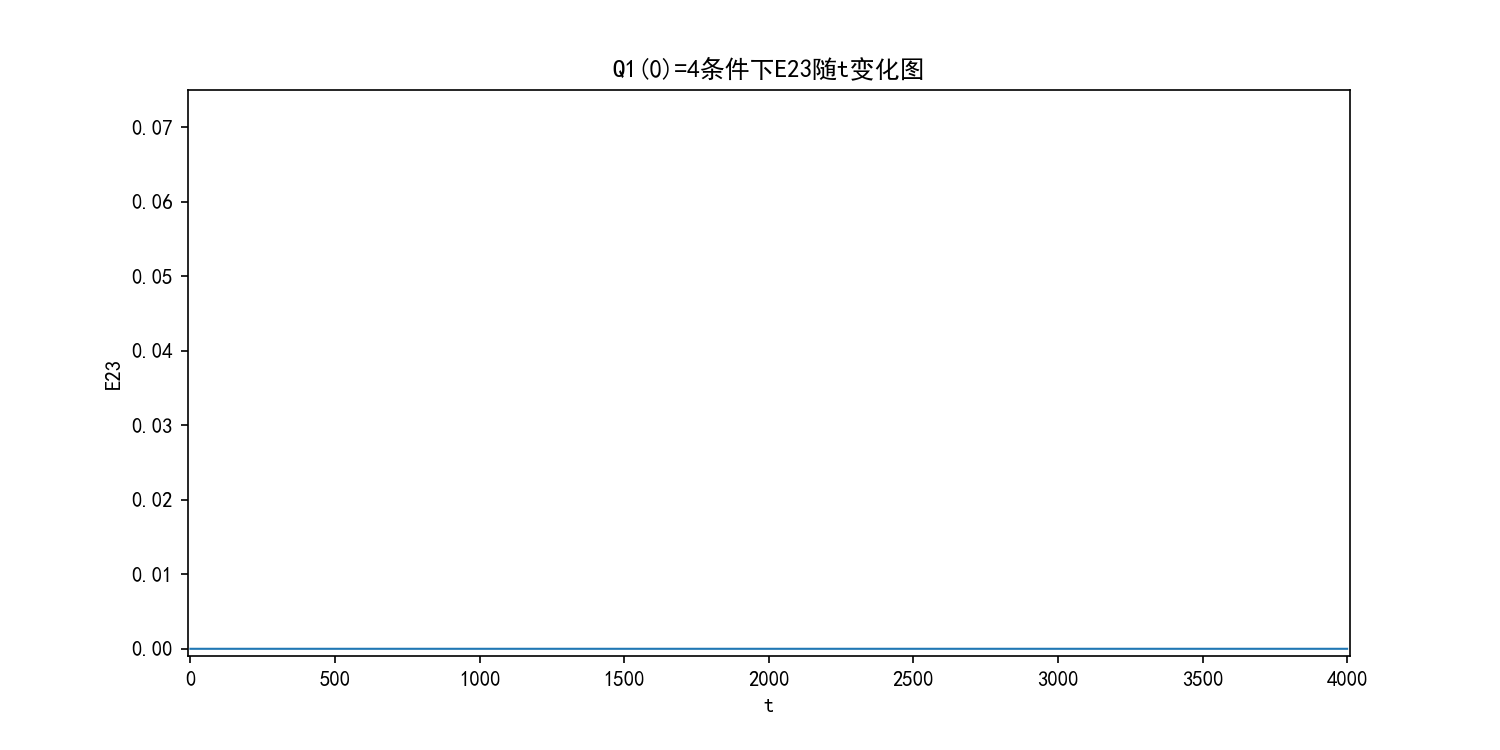
\includegraphics[width=\textwidth]{./q5_pics/cmp/E23.png}
        \end{minipage}
        \begin{minipage}[t]{0.49\textwidth}
            \centering
            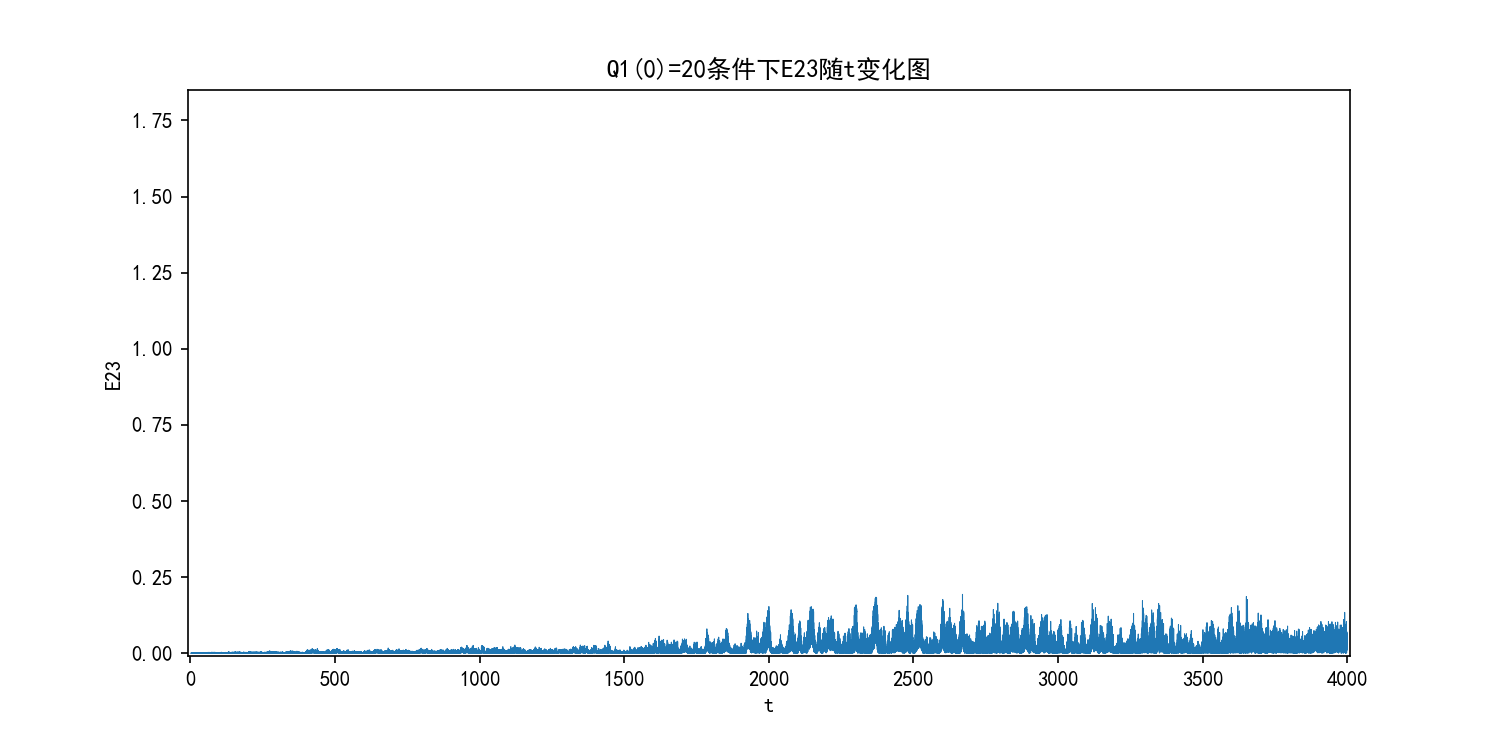
\includegraphics[width=\textwidth]{./q5_pics/exp/E23.png}
        \end{minipage}
        \caption{E23}\label{fig:E23 in q5}
    \end{figure}
    \begin{figure}[H]
        \begin{minipage}[t]{0.49\textwidth}
            \centering
            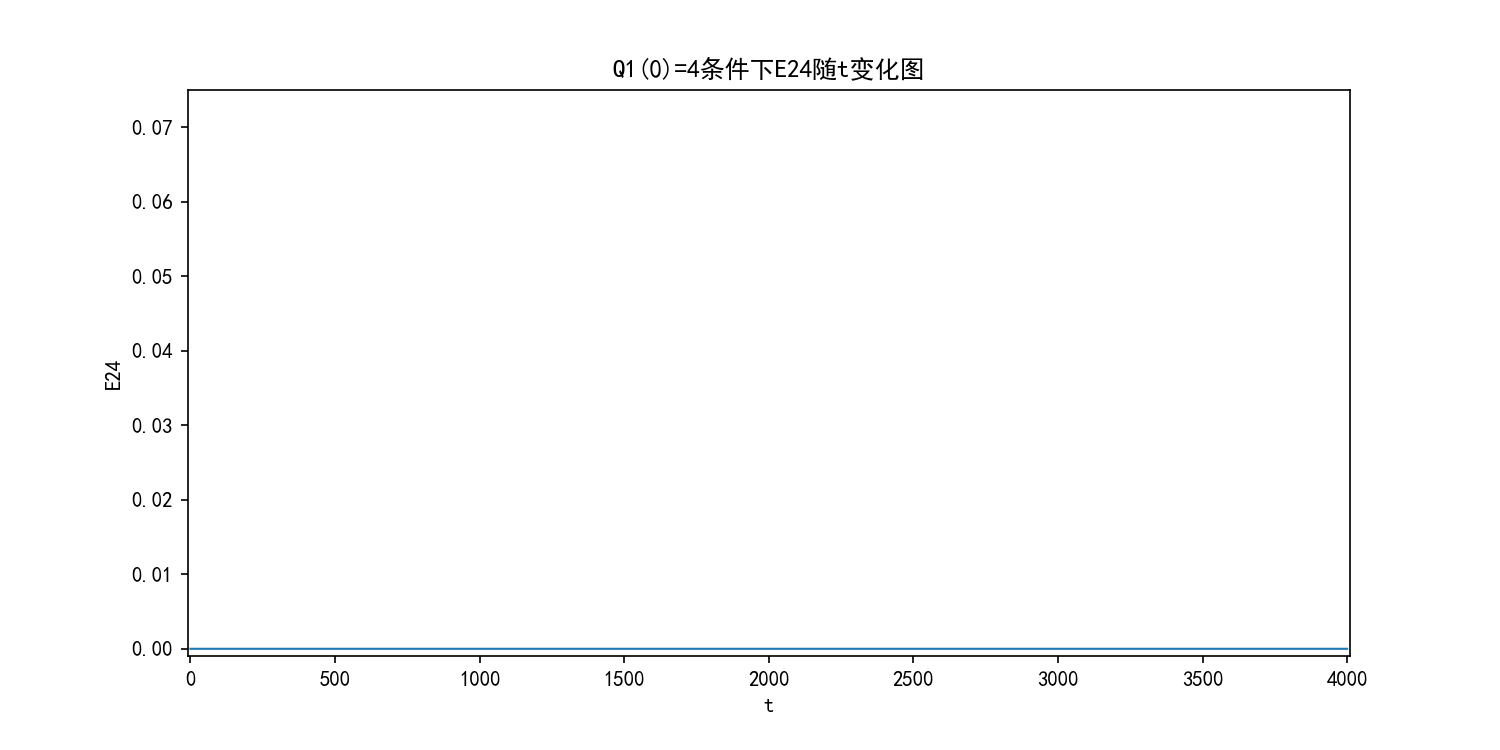
\includegraphics[width=\textwidth]{./q5_pics/cmp/E24.png}
        \end{minipage}
        \begin{minipage}[t]{0.49\textwidth}
            \centering
            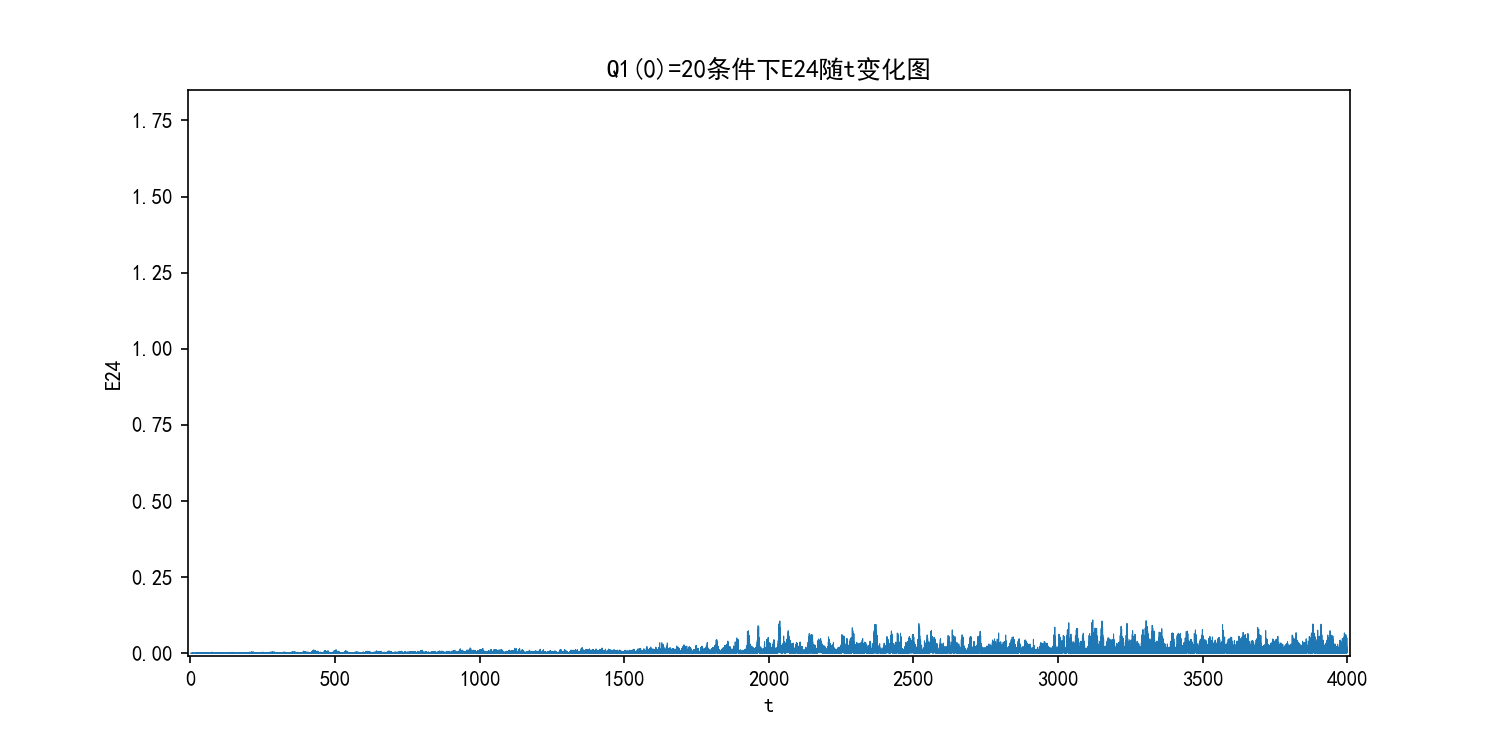
\includegraphics[width=\textwidth]{./q5_pics/exp/E24.png}
        \end{minipage}
        \caption{E24}\label{fig:E24 in q5}
    \end{figure}
    \begin{figure}[H]
        \begin{minipage}[t]{0.49\textwidth}
            \centering
            \includegraphics[width=\textwidth]{./q5_pics/cmp/E25.png}
        \end{minipage}
        \begin{minipage}[t]{0.49\textwidth}
            \centering
            \includegraphics[width=\textwidth]{./q5_pics/exp/E25.png}
        \end{minipage}
        \caption{E25}\label{fig:E25 in q5}
    \end{figure}
    \begin{figure}[H]
        \begin{minipage}[t]{0.49\textwidth}
            \centering
            \includegraphics[width=\textwidth]{./q5_pics/cmp/E26.png}
        \end{minipage}
        \begin{minipage}[t]{0.49\textwidth}
            \centering
            \includegraphics[width=\textwidth]{./q5_pics/exp/E26.png}
        \end{minipage}
        \caption{E26}\label{fig:E26 in q5}
    \end{figure}
    \begin{figure}[H]
        \begin{minipage}[t]{0.49\textwidth}
            \centering
            \includegraphics[width=\textwidth]{./q5_pics/cmp/E27.png}
        \end{minipage}
        \begin{minipage}[t]{0.49\textwidth}
            \centering
            \includegraphics[width=\textwidth]{./q5_pics/exp/E27.png}
        \end{minipage}
        \caption{E27}\label{fig:E27 in q5}
    \end{figure}
    \begin{figure}[H]
        \begin{minipage}[t]{0.49\textwidth}
            \centering
            \includegraphics[width=\textwidth]{./q5_pics/cmp/E28.png}
        \end{minipage}
        \begin{minipage}[t]{0.49\textwidth}
            \centering
            \includegraphics[width=\textwidth]{./q5_pics/exp/E28.png}
        \end{minipage}
        \caption{E28}\label{fig:E28 in q5}
    \end{figure}
    \begin{figure}[H]
        \begin{minipage}[t]{0.49\textwidth}
            \centering
            \includegraphics[width=\textwidth]{./q5_pics/cmp/E29.png}
        \end{minipage}
        \begin{minipage}[t]{0.49\textwidth}
            \centering
            \includegraphics[width=\textwidth]{./q5_pics/exp/E29.png}
        \end{minipage}
        \caption{E29}\label{fig:E29 in q5}
    \end{figure}
    \begin{figure}[H]
        \begin{minipage}[t]{0.49\textwidth}
            \centering
            \includegraphics[width=\textwidth]{./q5_pics/cmp/E30.png}
        \end{minipage}
        \begin{minipage}[t]{0.49\textwidth}
            \centering
            \includegraphics[width=\textwidth]{./q5_pics/exp/E30.png}
        \end{minipage}
        \caption{E30}\label{fig:E30 in q5}
    \end{figure}
    \begin{figure}[H]
        \begin{minipage}[t]{0.49\textwidth}
            \centering
            \includegraphics[width=\textwidth]{./q5_pics/cmp/E31.png}
        \end{minipage}
        \begin{minipage}[t]{0.49\textwidth}
            \centering
            \includegraphics[width=\textwidth]{./q5_pics/exp/E31.png}
        \end{minipage}
        \caption{E31}\label{fig:E31 in q5}
    \end{figure}
    \begin{figure}[H]
        \begin{minipage}[t]{0.49\textwidth}
            \centering
            \includegraphics[width=\textwidth]{./q5_pics/cmp/E32.png}
        \end{minipage}
        \begin{minipage}[t]{0.49\textwidth}
            \centering
            \includegraphics[width=\textwidth]{./q5_pics/exp/E32.png}
        \end{minipage}
        \caption{E32}\label{fig:E32 in q5}
    \end{figure}

    这里每一类初始条件各个模式均选取相同的纵坐标显示范围,可以直观比较出各个模式的强度。观察$E_1$至$E_4$,左侧图具有明显回归周期至3500,但右侧图中,保守的说,自t=500开始,系统就偏离了左侧的演化规律,呈现混乱状态。再观察其他能量右侧图,t=500之后,体系没有明显周期性规律可言。因此体系在大约t=500之后表现出混乱特征。

    同时,自上而下观察右侧图,可以看出初态$Q_1(0)=20$条件下,$<E_k>$随k的增大而减小。除了$E_{17},E_{18},E_{22}$部分区间有突然的增大之外,整体上这种单调关系是成立的。

    进一步的,如果对比左右两侧的图,可以发现初态$Q_1(0)=4$条件下基本没有能量转移到$E_9$之后的模式上,而初态$Q_1(0)=20$条件下能量在所有模式上都有转移,这和初态$Q_1(0)=20$条件得到的体系混乱程度更高是一致的。

    \subsection{第六问}

    这里只需要将第2、4、5问中的代码与非齐次项相关的地方作出修改即可。

    这里取n=32,$\beta=1$,初始条件$Q_1(0)=10$其他都为0为例。

    \subsubsection{类似第二问的结果}

    代码见附录"q6_to_q2.c",所得原始数据见"q6_to_q2.txt"
    \begin{figure}[H]
        \centering
        \includegraphics[width=0.8\textwidth]{第六问联系第二问图.jpg}
        \caption{第六问联系第二问图}\label{fig:第六问联系第二问图}
    \end{figure}

    可以看出一个回归周期t=85,能量比例$\eta=0.455/0.46182=98.5\%$。特别注意考虑到偶数模式为零,这里画出的是$E_1,E_3,E_5,E_7$随时间的变化。

    \subsubsection{类似第四问的结果}

    代码见附录"q6_to_q4.c",所得原始数据见"q6_to_q4.txt"
    \begin{figure}[H]
        \centering
        \includegraphics[width=0.8\textwidth]{第六问联系第四问图.jpg}
        \caption{第六问联系第四问图}\label{fig:第六问联系第四问图}
    \end{figure}

    可以看出一个回归周期t=433,能量比例$\eta=0.46105/0.46196=99.8\%$。与第四问类似,能量回归率大于小周期处。

    \subsubsection{类似第五问结果}

    重置$Q_1(0)=100$,将$Q_1(0)=10$和$Q_1(0)=100$各个模式能量在t从0-700(单位$2\pi/\omega_1$)的演化做对比,得到下图。代码见"q6_tp_q5.c",原始数据见"q6_tp_q5.txt",画图方法同第五问。

    \begin{figure}[H]
        \begin{minipage}[t]{0.49\textwidth}
            \centering
            \includegraphics[width=\textwidth]{./q6_pics/cmp/E1.png}
        \end{minipage}
        \begin{minipage}[t]{0.49\textwidth}
            \centering
            \includegraphics[width=\textwidth]{./q6_pics/exp/E1.png}
        \end{minipage}
        \caption{E1}\label{fig:E1 in q6}
    \end{figure}
    \begin{figure}[H]
        \begin{minipage}[t]{0.49\textwidth}
            \centering
            \includegraphics[width=\textwidth]{./q6_pics/cmp/E2.png}
        \end{minipage}
        \begin{minipage}[t]{0.49\textwidth}
            \centering
            \includegraphics[width=\textwidth]{./q6_pics/exp/E2.png}
        \end{minipage}
        \caption{E2}\label{fig:E2 in q6}
    \end{figure}
    \begin{figure}[H]
        \begin{minipage}[t]{0.49\textwidth}
            \centering
            \includegraphics[width=\textwidth]{./q6_pics/cmp/E3.png}
        \end{minipage}
        \begin{minipage}[t]{0.49\textwidth}
            \centering
            \includegraphics[width=\textwidth]{./q6_pics/exp/E3.png}
        \end{minipage}
        \caption{E3}\label{fig:E3 in q6}
    \end{figure}
    \begin{figure}[H]
        \begin{minipage}[t]{0.49\textwidth}
            \centering
            \includegraphics[width=\textwidth]{./q6_pics/cmp/E4.png}
        \end{minipage}
        \begin{minipage}[t]{0.49\textwidth}
            \centering
            \includegraphics[width=\textwidth]{./q6_pics/exp/E4.png}
        \end{minipage}
        \caption{E4}\label{fig:E4 in q6}
    \end{figure}
    \begin{figure}[H]
        \begin{minipage}[t]{0.49\textwidth}
            \centering
            \includegraphics[width=\textwidth]{./q6_pics/cmp/E5.png}
        \end{minipage}
        \begin{minipage}[t]{0.49\textwidth}
            \centering
            \includegraphics[width=\textwidth]{./q6_pics/exp/E5.png}
        \end{minipage}
        \caption{E5}\label{fig:E5 in q6}
    \end{figure}
    \begin{figure}[H]
        \begin{minipage}[t]{0.49\textwidth}
            \centering
            \includegraphics[width=\textwidth]{./q6_pics/cmp/E6.png}
        \end{minipage}
        \begin{minipage}[t]{0.49\textwidth}
            \centering
            \includegraphics[width=\textwidth]{./q6_pics/exp/E6.png}
        \end{minipage}
        \caption{E6}\label{fig:E6 in q6}
    \end{figure}
    \begin{figure}[H]
        \begin{minipage}[t]{0.49\textwidth}
            \centering
            \includegraphics[width=\textwidth]{./q6_pics/cmp/E7.png}
        \end{minipage}
        \begin{minipage}[t]{0.49\textwidth}
            \centering
            \includegraphics[width=\textwidth]{./q6_pics/exp/E7.png}
        \end{minipage}
        \caption{E7}\label{fig:E7 in q6}
    \end{figure}
    \begin{figure}[H]
        \begin{minipage}[t]{0.49\textwidth}
            \centering
            \includegraphics[width=\textwidth]{./q6_pics/cmp/E8.png}
        \end{minipage}
        \begin{minipage}[t]{0.49\textwidth}
            \centering
            \includegraphics[width=\textwidth]{./q6_pics/exp/E8.png}
        \end{minipage}
        \caption{E8}\label{fig:E8 in q6}
    \end{figure}
    \begin{figure}[H]
        \begin{minipage}[t]{0.49\textwidth}
            \centering
            \includegraphics[width=\textwidth]{./q6_pics/cmp/E9.png}
        \end{minipage}
        \begin{minipage}[t]{0.49\textwidth}
            \centering
            \includegraphics[width=\textwidth]{./q6_pics/exp/E9.png}
        \end{minipage}
        \caption{E9}\label{fig:E9 in q6}
    \end{figure}
    \begin{figure}[H]
        \begin{minipage}[t]{0.49\textwidth}
            \centering
            \includegraphics[width=\textwidth]{./q6_pics/cmp/E10.png}
        \end{minipage}
        \begin{minipage}[t]{0.49\textwidth}
            \centering
            \includegraphics[width=\textwidth]{./q6_pics/exp/E10.png}
        \end{minipage}
        \caption{E10}\label{fig:E10 in q6}
    \end{figure}
    \begin{figure}[H]
        \begin{minipage}[t]{0.49\textwidth}
            \centering
            \includegraphics[width=\textwidth]{./q6_pics/cmp/E11.png}
        \end{minipage}
        \begin{minipage}[t]{0.49\textwidth}
            \centering
            \includegraphics[width=\textwidth]{./q6_pics/exp/E11.png}
        \end{minipage}
        \caption{E11}\label{fig:E11 in q6}
    \end{figure}
    \begin{figure}[H]
        \begin{minipage}[t]{0.49\textwidth}
            \centering
            \includegraphics[width=\textwidth]{./q6_pics/cmp/E12.png}
        \end{minipage}
        \begin{minipage}[t]{0.49\textwidth}
            \centering
            \includegraphics[width=\textwidth]{./q6_pics/exp/E12.png}
        \end{minipage}
        \caption{E12}\label{fig:E12 in q6}
    \end{figure}
    \begin{figure}[H]
        \begin{minipage}[t]{0.49\textwidth}
            \centering
            \includegraphics[width=\textwidth]{./q6_pics/cmp/E13.png}
        \end{minipage}
        \begin{minipage}[t]{0.49\textwidth}
            \centering
            \includegraphics[width=\textwidth]{./q6_pics/exp/E13.png}
        \end{minipage}
        \caption{E13}\label{fig:E13 in q6}
    \end{figure}
    \begin{figure}[H]
        \begin{minipage}[t]{0.49\textwidth}
            \centering
            \includegraphics[width=\textwidth]{./q6_pics/cmp/E14.png}
        \end{minipage}
        \begin{minipage}[t]{0.49\textwidth}
            \centering
            \includegraphics[width=\textwidth]{./q6_pics/exp/E14.png}
        \end{minipage}
        \caption{E14}\label{fig:E14 in q6}
    \end{figure}
    \begin{figure}[H]
        \begin{minipage}[t]{0.49\textwidth}
            \centering
            \includegraphics[width=\textwidth]{./q6_pics/cmp/E15.png}
        \end{minipage}
        \begin{minipage}[t]{0.49\textwidth}
            \centering
            \includegraphics[width=\textwidth]{./q6_pics/exp/E15.png}
        \end{minipage}
        \caption{E15}\label{fig:E15 in q6}
    \end{figure}
    \begin{figure}[H]
        \begin{minipage}[t]{0.49\textwidth}
            \centering
            \includegraphics[width=\textwidth]{./q6_pics/cmp/E16.png}
        \end{minipage}
        \begin{minipage}[t]{0.49\textwidth}
            \centering
            \includegraphics[width=\textwidth]{./q6_pics/exp/E16.png}
        \end{minipage}
        \caption{E16}\label{fig:E16 in q6}
    \end{figure}
    \begin{figure}[H]
        \begin{minipage}[t]{0.49\textwidth}
            \centering
            \includegraphics[width=\textwidth]{./q6_pics/cmp/E17.png}
        \end{minipage}
        \begin{minipage}[t]{0.49\textwidth}
            \centering
            \includegraphics[width=\textwidth]{./q6_pics/exp/E17.png}
        \end{minipage}
        \caption{E17}\label{fig:E17 in q6}
    \end{figure}
    \begin{figure}[H]
        \begin{minipage}[t]{0.49\textwidth}
            \centering
            \includegraphics[width=\textwidth]{./q6_pics/cmp/E18.png}
        \end{minipage}
        \begin{minipage}[t]{0.49\textwidth}
            \centering
            \includegraphics[width=\textwidth]{./q6_pics/exp/E18.png}
        \end{minipage}
        \caption{E18}\label{fig:E18 in q6}
    \end{figure}
    \begin{figure}[H]
        \begin{minipage}[t]{0.49\textwidth}
            \centering
            \includegraphics[width=\textwidth]{./q6_pics/cmp/E19.png}
        \end{minipage}
        \begin{minipage}[t]{0.49\textwidth}
            \centering
            \includegraphics[width=\textwidth]{./q6_pics/exp/E19.png}
        \end{minipage}
        \caption{E19}\label{fig:E19 in q6}
    \end{figure}
    \begin{figure}[H]
        \begin{minipage}[t]{0.49\textwidth}
            \centering
            \includegraphics[width=\textwidth]{./q6_pics/cmp/E20.png}
        \end{minipage}
        \begin{minipage}[t]{0.49\textwidth}
            \centering
            \includegraphics[width=\textwidth]{./q6_pics/exp/E20.png}
        \end{minipage}
        \caption{E20}\label{fig:E20 in q6}
    \end{figure}
    \begin{figure}[H]
        \begin{minipage}[t]{0.49\textwidth}
            \centering
            \includegraphics[width=\textwidth]{./q6_pics/cmp/E21.png}
        \end{minipage}
        \begin{minipage}[t]{0.49\textwidth}
            \centering
            \includegraphics[width=\textwidth]{./q6_pics/exp/E21.png}
        \end{minipage}
        \caption{E21}\label{fig:E21 in q6}
    \end{figure}
    \begin{figure}[H]
        \begin{minipage}[t]{0.49\textwidth}
            \centering
            \includegraphics[width=\textwidth]{./q6_pics/cmp/E22.png}
        \end{minipage}
        \begin{minipage}[t]{0.49\textwidth}
            \centering
            \includegraphics[width=\textwidth]{./q6_pics/exp/E22.png}
        \end{minipage}
        \caption{E22}\label{fig:E22 in q6}
    \end{figure}
    \begin{figure}[H]
        \begin{minipage}[t]{0.49\textwidth}
            \centering
            \includegraphics[width=\textwidth]{./q6_pics/cmp/E23.png}
        \end{minipage}
        \begin{minipage}[t]{0.49\textwidth}
            \centering
            \includegraphics[width=\textwidth]{./q6_pics/exp/E23.png}
        \end{minipage}
        \caption{E23}\label{fig:E23 in q6}
    \end{figure}
    \begin{figure}[H]
        \begin{minipage}[t]{0.49\textwidth}
            \centering
            \includegraphics[width=\textwidth]{./q6_pics/cmp/E24.png}
        \end{minipage}
        \begin{minipage}[t]{0.49\textwidth}
            \centering
            \includegraphics[width=\textwidth]{./q6_pics/exp/E24.png}
        \end{minipage}
        \caption{E24}\label{fig:E24 in q6}
    \end{figure}
    \begin{figure}[H]
        \begin{minipage}[t]{0.49\textwidth}
            \centering
            \includegraphics[width=\textwidth]{./q6_pics/cmp/E25.png}
        \end{minipage}
        \begin{minipage}[t]{0.49\textwidth}
            \centering
            \includegraphics[width=\textwidth]{./q6_pics/exp/E25.png}
        \end{minipage}
        \caption{E25}\label{fig:E25 in q6}
    \end{figure}
    \begin{figure}[H]
        \begin{minipage}[t]{0.49\textwidth}
            \centering
            \includegraphics[width=\textwidth]{./q6_pics/cmp/E26.png}
        \end{minipage}
        \begin{minipage}[t]{0.49\textwidth}
            \centering
            \includegraphics[width=\textwidth]{./q6_pics/exp/E26.png}
        \end{minipage}
        \caption{E26}\label{fig:E26 in q6}
    \end{figure}
    \begin{figure}[H]
        \begin{minipage}[t]{0.49\textwidth}
            \centering
            \includegraphics[width=\textwidth]{./q6_pics/cmp/E27.png}
        \end{minipage}
        \begin{minipage}[t]{0.49\textwidth}
            \centering
            \includegraphics[width=\textwidth]{./q6_pics/exp/E27.png}
        \end{minipage}
        \caption{E27}\label{fig:E27 in q6}
    \end{figure}
    \begin{figure}[H]
        \begin{minipage}[t]{0.49\textwidth}
            \centering
            \includegraphics[width=\textwidth]{./q6_pics/cmp/E28.png}
        \end{minipage}
        \begin{minipage}[t]{0.49\textwidth}
            \centering
            \includegraphics[width=\textwidth]{./q6_pics/exp/E28.png}
        \end{minipage}
        \caption{E28}\label{fig:E28 in q6}
    \end{figure}
    \begin{figure}[H]
        \begin{minipage}[t]{0.49\textwidth}
            \centering
            \includegraphics[width=\textwidth]{./q6_pics/cmp/E29.png}
        \end{minipage}
        \begin{minipage}[t]{0.49\textwidth}
            \centering
            \includegraphics[width=\textwidth]{./q6_pics/exp/E29.png}
        \end{minipage}
        \caption{E29}\label{fig:E29 in q6}
    \end{figure}
    \begin{figure}[H]
        \begin{minipage}[t]{0.49\textwidth}
            \centering
            \includegraphics[width=\textwidth]{./q6_pics/cmp/E30.png}
        \end{minipage}
        \begin{minipage}[t]{0.49\textwidth}
            \centering
            \includegraphics[width=\textwidth]{./q6_pics/exp/E30.png}
        \end{minipage}
        \caption{E30}\label{fig:E30 in q6}
    \end{figure}
    \begin{figure}[H]
        \begin{minipage}[t]{0.49\textwidth}
            \centering
            \includegraphics[width=\textwidth]{./q6_pics/cmp/E31.png}
        \end{minipage}
        \begin{minipage}[t]{0.49\textwidth}
            \centering
            \includegraphics[width=\textwidth]{./q6_pics/exp/E31.png}
        \end{minipage}
        \caption{E31}\label{fig:E31 in q6}
    \end{figure}
    \begin{figure}[H]
        \begin{minipage}[t]{0.49\textwidth}
            \centering
            \includegraphics[width=\textwidth]{./q6_pics/cmp/E32.png}
        \end{minipage}
        \begin{minipage}[t]{0.49\textwidth}
            \centering
            \includegraphics[width=\textwidth]{./q6_pics/exp/E32.png}
        \end{minipage}
        \caption{E32}\label{fig:E32 in q6}
    \end{figure}

    可以看出改变初态后,体系周期性被显著打破,体现出混沌的特性。

    \subsection{第七问}
    由前问-类似第五问结果中的左侧图可以看出,当初始模式能量集中在模式1时,偶数次
    模式能量始终为零,但是如果改变初条件如前问右侧图所示,这种奇偶锁定就破坏了,这与下面的计算得到的结论相仿。

    本问计算与前问相仿,只需改变参数n即可,代码见"q7.c",运行结果见"q7.txt"(注意这里要用科学计数法输出数据)。

    我们还取t的单位为$2\pi/\omega_1$,得到下图。

    \begin{figure}[H]
        \centering
        \includegraphics[width=0.8\textwidth]{第七问图.jpg}
        \caption{第七问图}\label{fig:第七问图}
    \end{figure}

    可以看出,随着时间演化,偶数次模式的能量的计算结果不断上升,最终与奇数次模式能量的量级相当,达到混乱状态。可能是由于舍入误差和蛙跳法的精度带来的误差影响下,偶数次模式能量不断获得一些噪声并逐渐积累变大导致。

    \subsection{第八问}

    这里时间仍取$2\pi/\omega_1$为单位,可以每隔0.1时间打出一个所有质点的位移,总共打200份时间。代码见"q8.c",原始数据见"q8_beta=0.txt"($\beta=0$),"q8_beta=1.txt"($\beta=1$)。

    这里可以对每个时刻,以位移为纵坐标、质点编号为横坐标画图,进而可以观察波的演化,应用"q8_beta=0.txt""q8_beta=1.txt"我们已经可以得到所有的波随时间演化的信息了。为方便绘图,我们同样借助python,源代码见附录"q8.py"。

    这样可以得到每个时刻波的位形图,应用ScreenToGif软件,将所有帧连成视频,得到$\beta=0$和$\beta=1$波的演化视频,见"q8_beta=0.mp4""q8_beta=1.mp4"

    可以看出,当$\beta=0$时,没有非线性效应,波在传播过程中会逐渐弥散;而当$\beta=1$时,波能够维持原来的形状随时间演化!

    \section{附录(源代码)}

    以下所有C程序均引用了"matrix.h"包,由于这个包较长,这里不再列出,而把源文件附在文件夹中,详见"matrix.h"
    \subsection{"q2.c"}

    \begin{lstlisting}[language=C]
#include "matrix.h"
#define NUM 32
#define alpha 0.25
#define SCALE 1e+3

double dt;

double dqH(int j,vector* q){
    if(j<0||j>NUM-1){printf("wrong index: the index of the vector entry should be in range 0 to NUM-1\n");return 0;}
    switch (j)
    {
    case 0:
        return -(q->el[j]-q->el[j+1])-q->el[j]-alpha*pow((q->el[j]-q->el[j+1]),2)+alpha*pow((q->el[j]),2);
        break;

    case NUM-1:
        return -(q->el[j])+(q->el[j-1]-q->el[j])-alpha*pow((q->el[j]),2)+alpha*pow((q->el[j-1]-q->el[j]),2);
        break;
    
    default:
        return -(q->el[j]-q->el[j+1])+(q->el[j-1]-q->el[j])-alpha*pow((q->el[j]-q->el[j+1]),2)+alpha*pow((q->el[j-1]-q->el[j]),2);
        break;
    }
}

double eigen_transform(SqMatrix* A,vector* b,int k){
	if(A->n!=b->n)return 0;
    int i;
    double s=0;
    for ( i = 0; i < b->n ; i++)
    {
        s+=A->el[k][i]*b->el[i];
    }
    return s;
}

int main(){
    dt=PI/sin(PI/(2*(NUM+1)))/SCALE;
    FILE* fdata=fopen("C:/C_files/HW4/q5_cmp_sparsify.txt","w");
    SqMatrix* A=createZeroSqMatrix(NUM);
    int i,j,k;
    for ( k = 0; k < NUM; k++)
    {
        for ( j = 0; j < NUM; j++)
        {
            A->el[k][j]=sqrt(2./(NUM+1))*sin(PI*(k+1)*(j+1)/(NUM+1));
        }
    }
    SqMatrix* Acopy=createZeroSqMatrix(NUM);
    copy_SqMatrix(A,Acopy);
	
    vector* q=createNewVector(NUM);
    q->el[0]=4;
    if(Solve_RankN_LinearEq(A,q)){
        print_vector(q);
    }
    vector* p=createNewVector(NUM);

    fprintf(fdata,"0\t");
    
    for ( i=0;i<4;i++)
    {
        double Qk=eigen_transform(Acopy,q,i);
        double Pk=eigen_transform(Acopy,p,i);
        double wk=2*sin((i+1)*PI/2/(NUM+1));
        double Ek=0.5*Pk*Pk+0.5*pow(wk*Qk,2);
        fprintf(fdata,"%lf\t",Ek);
        
    }
    fprintf(fdata,"\n");
    

    vector* pf, *pr;
    pr=createNewVector(NUM);
    pf=createNewVector(NUM);
    for ( j = 0; j < NUM; j++)
    {
        pf->el[j]=0.5*dt*dqH(j,q);
    }
    
    for(i=1;i<=160*SCALE;i++){
        copy_vector(pf,pr);
        for ( j = 0; j < NUM; j++)
        {
            q->el[j]+=(pr->el[j]*dt);
        }
        for ( j = 0; j < NUM; j++){
            pf->el[j]=pr->el[j]+dt*dqH(j,q);
        }
        average_vector(pr,pf,p);
        fprintf(fdata,"%lf\t",(double)i/SCALE);
        for ( k=0;k<4;k++)
        {
            double Qk=eigen_transform(Acopy,q,k);
            double Pk=eigen_transform(Acopy,p,k);
            double wk=2*sin((k+1)*PI/2/(NUM+1));
            double Ek=0.5*Pk*Pk+0.5*pow(wk*Qk,2);
            fprintf(fdata,"%lf\t",Ek);
        }
        fprintf(fdata,"\n");
    }
    return 0;
}

    \end{lstlisting}


    \subsection{"q4.c"}

    \begin{lstlisting}[language=C]
#include "matrix.h"
#define NUM 32
#define alpha 0.25
#define SCALE 1e+3

double dt;

double dqH(int j,vector* q){
    if(j<0||j>NUM-1){printf("wrong index: the index of the vector entry should be in range 0 to NUM-1\n");return 0;}
    switch (j)
    {
    case 0:
        return -(q->el[j]-q->el[j+1])-q->el[j]-alpha*pow((q->el[j]-q->el[j+1]),2)+alpha*pow((q->el[j]),2);
        break;

    case NUM-1:
        return -(q->el[j])+(q->el[j-1]-q->el[j])-alpha*pow((q->el[j]),2)+alpha*pow((q->el[j-1]-q->el[j]),2);
        break;
    
    default:
        return -(q->el[j]-q->el[j+1])+(q->el[j-1]-q->el[j])-alpha*pow((q->el[j]-q->el[j+1]),2)+alpha*pow((q->el[j-1]-q->el[j]),2);
        break;
    }
}


double eigen_transform(SqMatrix* A,vector* b,int k){
    if(A->n!=b->n)return 0;
    int i;
    double s=0;
    for ( i = 0; i < b->n ; i++)
    {
        s+=A->el[k][i]*b->el[i];
    }
    return s;
}

int main(){
    dt=PI/sin(PI/(2*(NUM+1)))/SCALE;
    FILE* fdata=fopen("C:/C_files/HW4/q4.txt","w");
    SqMatrix* A=createZeroSqMatrix(NUM);
    int i,j,k;
    for ( k = 0; k < NUM; k++)
    {
        for ( j = 0; j < NUM; j++)
        {
            A->el[k][j]=sqrt(2./(NUM+1))*sin(PI*(k+1)*(j+1)/(NUM+1));
        }
    }
    SqMatrix* Acopy=createZeroSqMatrix(NUM);
    copy_SqMatrix(A,Acopy);
    
    vector* q=createNewVector(NUM);
    q->el[0]=4;
    if(Solve_RankN_LinearEq(A,q)){
        print_vector(q);
    }
    vector* p=createNewVector(NUM);

    fprintf(fdata,"0\t");
    
    double Qk=eigen_transform(Acopy,q,0);
    double Pk=eigen_transform(Acopy,p,0);
    double wk=2*sin(PI/2/(NUM+1));
    double Ek=0.5*Pk*Pk+0.5*pow(wk*Qk,2);
    fprintf(fdata,"%lf\t",Ek);
        
    fprintf(fdata,"\n");
    

    vector* pf, *pr;
    pr=createNewVector(NUM);
    pf=createNewVector(NUM);
    for ( j = 0; j < NUM; j++)
    {
        pf->el[j]=0.5*dt*dqH(j,q);
    }
    
    for(i=1;i<=4000*SCALE;i++){
        copy_vector(pf,pr);
        for ( j = 0; j < NUM; j++)
        {
            q->el[j]+=(pr->el[j]*dt);
        }
        for ( j = 0; j < NUM; j++){
            pf->el[j]=pr->el[j]+dt*dqH(j,q);
        }
            average_vector(pr,pf,p);
            fprintf(fdata,"%lf\t",(double)i/SCALE);

            double Qk=eigen_transform(Acopy,q,0);
            double Pk=eigen_transform(Acopy,p,0);
            double wk=2*sin(PI/2/(NUM+1));
            double Ek=0.5*Pk*Pk+0.5*pow(wk*Qk,2);
            fprintf(fdata,"%lf\t",Ek);
            fprintf(fdata,"\n");
    }
    return 0;
}    
    \end{lstlisting}

    \subsection{"q5.c"}

    \begin{lstlisting}[language=C]
#include "matrix.h"
#define NUM 32
#define OBSERVE 32
#define alpha 0.25
#define SCALE 1e+3

double dt;

double dqH(int j,vector* q){
    if(j<0||j>NUM-1){printf("wrong index: the index of the vector entry should be in range 0 to NUM-1\n");return 0;}
    switch (j)
    {
    case 0:
        return -(q->el[j]-q->el[j+1])-q->el[j]-alpha*pow((q->el[j]-q->el[j+1]),2)+alpha*pow((q->el[j]),2);
        break;

    case NUM-1:
        return -(q->el[j])+(q->el[j-1]-q->el[j])-alpha*pow((q->el[j]),2)+alpha*pow((q->el[j-1]-q->el[j]),2);
        break;
    
    default:
        return -(q->el[j]-q->el[j+1])+(q->el[j-1]-q->el[j])-alpha*pow((q->el[j]-q->el[j+1]),2)+alpha*pow((q->el[j-1]-q->el[j]),2);
        break;
    }
}


double eigen_transform(SqMatrix* A,vector* b,int k){
    if(A->n!=b->n)return 0;
    int i;
    double s=0;
    for ( i = 0; i < b->n ; i++)
    {
        s+=A->el[k][i]*b->el[i];
    }
    return s;
}

int main(){
    dt=PI/sin(PI/(2*(NUM+1)))/SCALE;
    FILE* fdata=fopen("C:/C_files/HW4/q5_cmp_sparsify.txt","w");
    SqMatrix* A=createZeroSqMatrix(NUM);
    int i,j,k;
    for ( k = 0; k < NUM; k++)
    {
        for ( j = 0; j < NUM; j++)
        {
            A->el[k][j]=sqrt(2./(NUM+1))*sin(PI*(k+1)*(j+1)/(NUM+1));
        }
    }
    SqMatrix* Acopy=createZeroSqMatrix(NUM);
    copy_SqMatrix(A,Acopy);
    
    vector* q=createNewVector(NUM);
    q->el[0]=4;
    if(Solve_RankN_LinearEq(A,q)){
        print_vector(q);
    }
    vector* p=createNewVector(NUM);

    fprintf(fdata,"0\t");
    
    for ( i=0;i<OBSERVE;i++)
    {
        double Qk=eigen_transform(Acopy,q,i);
        double Pk=eigen_transform(Acopy,p,i);
        double wk=2*sin((i+1)*PI/2/(NUM+1));
        double Ek=0.5*Pk*Pk+0.5*pow(wk*Qk,2);
        fprintf(fdata,"%lf\t",Ek);
        
    }
        
    fprintf(fdata,"\n");
    

    vector* pf, *pr;
    pr=createNewVector(NUM);
    pf=createNewVector(NUM);
    for ( j = 0; j < NUM; j++)
    {
        pf->el[j]=0.5*dt*dqH(j,q);
    }
    
    for(i=1;i<=4000*SCALE;i++){
        copy_vector(pf,pr);
        for ( j = 0; j < NUM; j++)
        {
            q->el[j]+=(pr->el[j]*dt);
        }
        for ( j = 0; j < NUM; j++){
            pf->el[j]=pr->el[j]+dt*dqH(j,q);
        }
        average_vector(pr,pf,p);
        
        if(i%10==0){
            fprintf(fdata,"%lf\t",(double)i/SCALE);
            for ( k=0;k<OBSERVE;k++)
            {
                double Qk=eigen_transform(Acopy,q,k);
                double Pk=eigen_transform(Acopy,p,k);
                double wk=2*sin((k+1)*PI/2/(NUM+1));
                double Ek=0.5*Pk*Pk+0.5*pow(wk*Qk,2);
                fprintf(fdata,"%lf\t",Ek);
            }
            fprintf(fdata,"\n");
        }
    }
    return 0;
}  
    \end{lstlisting}

    \subsection{"plotTool.py"}
    \begin{lstlisting}[language=Python]
import matplotlib.pyplot as plt
import numpy as np

plt.rcParams["font.sans-serif"]=["SimHei"]
plt.rcParams["axes.unicode_minus"]=False
a = np.loadtxt("C:/C_files/HW4/q6_to_q5_cmp.txt")

for i in range(32):
    plt.figure(figsize=(10,5),dpi=150)
    plt.xlim(-10,710)
    plt.ylim(-0.01,0.5)
    plt.xlabel("t")
    plt.ylabel("E"+str(int(i+1)))
    plt.title(chr(946)+"-FPU,""Q1(0)=10条件下E"+str(int(i+1))+"随t变化图")
    plt.plot(a[:,0],a[:,i+1],linewidth=0.5)
    plt.savefig("C:\\C_files\\HW4\\report\\q6_pics\\cmp\\E"+str(int(i+1))+".png")
    \end{lstlisting}

    \subsection{"q6_to_q2.c"}

    \begin{lstlisting}[language=C]
#include "matrix.h"
#define NUM 32
#define beta 1
#define SCALE 1e+3

double dt;

double dqH(int j,vector* q){
    if(j<0||j>NUM-1){printf("wrong index: the index of the vector entry should be in range 0 to NUM-1\n");return 0;}
    switch (j)
    {
    case 0:
        return -(q->el[j]-q->el[j+1])-q->el[j]-beta*pow((q->el[j]-q->el[j+1]),3)+beta*pow((-q->el[j]),3);
        break;

    case NUM-1:
        return -(q->el[j])+(q->el[j-1]-q->el[j])-beta*pow((q->el[j]),3)+beta*pow((q->el[j-1]-q->el[j]),3);
        break;
    
    default:
        return -(q->el[j]-q->el[j+1])+(q->el[j-1]-q->el[j])-beta*pow((q->el[j]-q->el[j+1]),3)+beta*pow((q->el[j-1]-q->el[j]),3);
        break;
    }
}

double eigen_transform(SqMatrix* A,vector* b,int k){
	if(A->n!=b->n)return 0;
    int i;
    double s=0;
    for ( i = 0; i < b->n ; i++)
    {
        s+=A->el[k][i]*b->el[i];
    }
    return s;
}

int main(){
    dt=PI/sin(PI/(2*(NUM+1)))/SCALE;
    FILE* fdata=fopen("C:/C_files/HW4/q6_to_q2.txt","w");
    SqMatrix* A=createZeroSqMatrix(NUM);
    int i,j,k;
    for ( k = 0; k < NUM; k++)
    {
        for ( j = 0; j < NUM; j++)
        {
            A->el[k][j]=sqrt(2./(NUM+1))*sin(PI*(k+1)*(j+1)/(NUM+1));
        }
    }
    SqMatrix* Acopy=createZeroSqMatrix(NUM);
    copy_SqMatrix(A,Acopy);
	
    vector* q=createNewVector(NUM);
    q->el[0]=10;
    if(Solve_RankN_LinearEq(A,q)){
        print_vector(q);
    }
    vector* p=createNewVector(NUM);

    fprintf(fdata,"0\t");
    
    for ( i=0;i<7;i+=2)
    {
        double Qk=eigen_transform(Acopy,q,i);
        double Pk=eigen_transform(Acopy,p,i);
        double wk=2*sin((i+1)*PI/2/(NUM+1));
        double Ek=0.5*Pk*Pk+0.5*pow(wk*Qk,2);
        fprintf(fdata,"%lf\t",Ek);
        
    }
    fprintf(fdata,"\n");
    

    vector* pf, *pr;
    pr=createNewVector(NUM);
    pf=createNewVector(NUM);
    for ( j = 0; j < NUM; j++)
    {
        pf->el[j]=0.5*dt*dqH(j,q);
    }
    
    for(i=1;i<=100*SCALE;i++){
        copy_vector(pf,pr);
        for ( j = 0; j < NUM; j++)
        {
            q->el[j]+=(pr->el[j]*dt);
        }
        for ( j = 0; j < NUM; j++){
            pf->el[j]=pr->el[j]+dt*dqH(j,q);
        }
        average_vector(pr,pf,p);
        fprintf(fdata,"%lf\t",(double)i/SCALE);
        for ( k=0;k<7;k+=2)
        {
            double Qk=eigen_transform(Acopy,q,k);
            double Pk=eigen_transform(Acopy,p,k);
            double wk=2*sin((k+1)*PI/2/(NUM+1));
            double Ek=0.5*Pk*Pk+0.5*pow(wk*Qk,2);
            fprintf(fdata,"%lf\t",Ek);
        }
        fprintf(fdata,"\n");
    }
    return 0;
}
    \end{lstlisting}

    \subsection{"q6_to_q4.c"}
    \begin{lstlisting}[language=C]
#include "matrix.h"
#define NUM 32
#define beta 1
#define SCALE 1e+4

double dt;

double dqH(int j,vector* q){
    if(j<0||j>NUM-1){printf("wrong index: the index of the vector entry should be in range 0 to NUM-1\n");return 0;}
    switch (j)
    {
    case 0:
        return -(q->el[j]-q->el[j+1])-q->el[j]-beta*pow((q->el[j]-q->el[j+1]),3)+beta*pow((-q->el[j]),3);
        break;

    case NUM-1:
        return -(q->el[j])+(q->el[j-1]-q->el[j])-beta*pow((q->el[j]),3)+beta*pow((q->el[j-1]-q->el[j]),3);
        break;
    
    default:
        return -(q->el[j]-q->el[j+1])+(q->el[j-1]-q->el[j])-beta*pow((q->el[j]-q->el[j+1]),3)+beta*pow((q->el[j-1]-q->el[j]),3);
        break;
    }
}

double eigen_transform(SqMatrix* A,vector* b,int k){
	if(A->n!=b->n)return 0;
    int i;
    double s=0;
    for ( i = 0; i < b->n ; i++)
    {
        s+=A->el[k][i]*b->el[i];
    }
    return s;
}

int main(){
    dt=PI/sin(PI/(2*(NUM+1)))/SCALE;
    FILE* fdata=fopen("C:/C_files/HW4/q6_to_q4.txt","w");
    SqMatrix* A=createZeroSqMatrix(NUM);
    int i,j,k;
    for ( k = 0; k < NUM; k++)
    {
        for ( j = 0; j < NUM; j++)
        {
            A->el[k][j]=sqrt(2./(NUM+1))*sin(PI*(k+1)*(j+1)/(NUM+1));
        }
    }
    SqMatrix* Acopy=createZeroSqMatrix(NUM);
    copy_SqMatrix(A,Acopy);
	
    vector* q=createNewVector(NUM);
    q->el[0]=10;
    if(Solve_RankN_LinearEq(A,q)){
        print_vector(q);
    }
    vector* p=createNewVector(NUM);

    fprintf(fdata,"0\t");
    
   
    double Qk=eigen_transform(Acopy,q,0);
    double Pk=eigen_transform(Acopy,p,0);
    double wk=2*sin(PI/2/(NUM+1));
    double Ek=0.5*Pk*Pk+0.5*pow(wk*Qk,2);
    fprintf(fdata,"%lf\t",Ek);

    fprintf(fdata,"\n");
    

    vector* pf, *pr;
    pr=createNewVector(NUM);
    pf=createNewVector(NUM);
    for ( j = 0; j < NUM; j++)
    {
        pf->el[j]=0.5*dt*dqH(j,q);
    }
    
    for(i=1;i<=700*SCALE;i++){
        copy_vector(pf,pr);
        for ( j = 0; j < NUM; j++)
        {
            q->el[j]+=(pr->el[j]*dt);
        }
        for ( j = 0; j < NUM; j++){
            pf->el[j]=pr->el[j]+dt*dqH(j,q);
        }
        average_vector(pr,pf,p);

        if(i%10==0){
            fprintf(fdata,"%lf\t",(double)i/SCALE);

            double Qk=eigen_transform(Acopy,q,0);
            double Pk=eigen_transform(Acopy,p,0);
            double wk=2*sin(PI/2/(NUM+1));
            double Ek=0.5*Pk*Pk+0.5*pow(wk*Qk,2);
            fprintf(fdata,"%lf\t",Ek);

            fprintf(fdata,"\n");
        }
        
    }
    return 0;
}
    \end{lstlisting}

    \subsection{"q6_to_q5.c"}
    \begin{lstlisting}[language=C]
#include "matrix.h"
#define NUM 32
#define OBSERVE 32
#define beta 1
#define SCALE 1e+3

double dt;

double dqH(int j,vector* q){
    if(j<0||j>NUM-1){printf("wrong index: the index of the vector entry should be in range 0 to NUM-1\n");return 0;}
    switch (j)
    {
    case 0:
        return -(q->el[j]-q->el[j+1])-q->el[j]-beta*pow((q->el[j]-q->el[j+1]),3)+beta*pow((-q->el[j]),3);
        break;

    case NUM-1:
        return -(q->el[j])+(q->el[j-1]-q->el[j])-beta*pow((q->el[j]),3)+beta*pow((q->el[j-1]-q->el[j]),3);
        break;
    
    default:
        return -(q->el[j]-q->el[j+1])+(q->el[j-1]-q->el[j])-beta*pow((q->el[j]-q->el[j+1]),3)+beta*pow((q->el[j-1]-q->el[j]),3);
        break;
    }
}

double eigen_transform(SqMatrix* A,vector* b,int k){
	if(A->n!=b->n)return 0;
    int i;
    double s=0;
    for ( i = 0; i < b->n ; i++)
    {
        s+=A->el[k][i]*b->el[i];
    }
    return s;
}

int main(){
    dt=PI/sin(PI/(2*(NUM+1)))/SCALE;
    FILE* fdata=fopen("C:/C_files/HW4/q6_to_q5.txt","w");
    SqMatrix* A=createZeroSqMatrix(NUM);
    int i,j,k;
    for ( k = 0; k < NUM; k++)
    {
        for ( j = 0; j < NUM; j++)
        {
            A->el[k][j]=sqrt(2./(NUM+1))*sin(PI*(k+1)*(j+1)/(NUM+1));
        }
    }
    SqMatrix* Acopy=createZeroSqMatrix(NUM);
    copy_SqMatrix(A,Acopy);
	
    vector* q=createNewVector(NUM);
    q->el[0]=100;
    if(Solve_RankN_LinearEq(A,q)){
        print_vector(q);
    }
    vector* p=createNewVector(NUM);

    fprintf(fdata,"0\t");
    
   for ( i=0;i<OBSERVE;i++)
    {
        double Qk=eigen_transform(Acopy,q,i);
        double Pk=eigen_transform(Acopy,p,i);
        double wk=2*sin((i+1)*PI/2/(NUM+1));
        double Ek=0.5*Pk*Pk+0.5*pow(wk*Qk,2);
        fprintf(fdata,"%lf\t",Ek);
        
    }

    fprintf(fdata,"\n");
    
    vector* pf, *pr;
    pr=createNewVector(NUM);
    pf=createNewVector(NUM);
    for ( j = 0; j < NUM; j++)
    {
        pf->el[j]=0.5*dt*dqH(j,q);
    }
    
    for(i=1;i<=700*SCALE;i++){
        copy_vector(pf,pr);
        for ( j = 0; j < NUM; j++)
        {
            q->el[j]+=(pr->el[j]*dt);
        }
        for ( j = 0; j < NUM; j++){
            pf->el[j]=pr->el[j]+dt*dqH(j,q);
        }
        
        if(i%10==0){
            average_vector(pr,pf,p);
            fprintf(fdata,"%lf\t",(double)i/SCALE);

           for ( k=0;k<OBSERVE;k++)
            {
                double Qk=eigen_transform(Acopy,q,k);
                double Pk=eigen_transform(Acopy,p,k);
                double wk=2*sin((k+1)*PI/2/(NUM+1));
                double Ek=0.5*Pk*Pk+0.5*pow(wk*Qk,2);
                fprintf(fdata,"%lf\t",Ek);
                
            }

            fprintf(fdata,"\n");
        }
    }

    return 0;
}
    \end{lstlisting}

    \subsection{"q7.c"}
    \begin{lstlisting}[language=C]
#include "matrix.h"
#define NUM 16
#define beta 1
#define SCALE 1e+4

double dt;

double dqH(int j,vector* q){
    if(j<0||j>NUM-1){printf("wrong index: the index of the vector entry should be in range 0 to NUM-1\n");return 0;}
    switch (j)
    {
    case 0:
        return -(q->el[j]-q->el[j+1])-q->el[j]-beta*pow((q->el[j]-q->el[j+1]),3)+beta*pow((-q->el[j]),3);
        break;

    case NUM-1:
        return -(q->el[j])+(q->el[j-1]-q->el[j])-beta*pow((q->el[j]),3)+beta*pow((q->el[j-1]-q->el[j]),3);
        break;
    
    default:
        return -(q->el[j]-q->el[j+1])+(q->el[j-1]-q->el[j])-beta*pow((q->el[j]-q->el[j+1]),3)+beta*pow((q->el[j-1]-q->el[j]),3);
        break;
    }
}

double eigen_transform(SqMatrix* A,vector* b,int k){
	if(A->n!=b->n)return 0;
    int i;
    double s=0;
    for ( i = 0; i < b->n ; i++)
    {
        s+=A->el[k][i]*b->el[i];
    }
    return s;
}

int main(){
    dt=PI/sin(PI/(2*(NUM+1)))/SCALE;
    FILE* fdata=fopen("C:/C_files/HW4/q7_intensify.txt","w");
    SqMatrix* A=createZeroSqMatrix(NUM);
    int i,j,k;
    for ( k = 0; k < NUM; k++)
    {
        for ( j = 0; j < NUM; j++)
        {
            A->el[k][j]=sqrt(2./(NUM+1))*sin(PI*(k+1)*(j+1)/(NUM+1));
        }
    }
    SqMatrix* Acopy=createZeroSqMatrix(NUM);
    copy_SqMatrix(A,Acopy);
	
    vector* q=createNewVector(NUM);
    q->el[10]=1;
    if(Solve_RankN_LinearEq(A,q)){
        print_vector(q);
    }
    vector* p=createNewVector(NUM);

    fprintf(fdata,"0\t");
    
    for ( i=8;i<13;i++)
    {
        double Qk=eigen_transform(Acopy,q,i);
        double Pk=eigen_transform(Acopy,p,i);
        double wk=2*sin((i+1)*PI/2/(NUM+1));
        double Ek=0.5*Pk*Pk+0.5*pow(wk*Qk,2);
        fprintf(fdata,"%e\t",Ek);
        
    }
    fprintf(fdata,"\n");
    

    vector* pf, *pr;
    pr=createNewVector(NUM);
    pf=createNewVector(NUM);
    for ( j = 0; j < NUM; j++)
    {
        pf->el[j]=0.5*dt*dqH(j,q);
    }
    
    for(i=1;i<=100*SCALE;i++){
        copy_vector(pf,pr);
        for ( j = 0; j < NUM; j++)
        {
            q->el[j]+=(pr->el[j]*dt);
        }
        for ( j = 0; j < NUM; j++){
            pf->el[j]=pr->el[j]+dt*dqH(j,q);
        }
        average_vector(pr,pf,p);
        fprintf(fdata,"%lf\t",(double)i/SCALE);
        for ( k=8;k<13;k++)
        {
            double Qk=eigen_transform(Acopy,q,k);
            double Pk=eigen_transform(Acopy,p,k);
            double wk=2*sin((k+1)*PI/2/(NUM+1));
            double Ek=0.5*Pk*Pk+0.5*pow(wk*Qk,2);
            fprintf(fdata,"%e\t",Ek);
        }
        fprintf(fdata,"\n");
    }
    return 0;
}
    \end{lstlisting}

    \subsection{"q8.c"}
    \begin{lstlisting}[language=C]
#include "matrix.h"
#define NUM 128
#define BETA 0
#define K 11
#define B 0.5
#define SCALE 1e+3



double dt;
double wk;

double dqH(int j,vector* q){
    if(j<0||j>NUM-1){printf("wrong index: the index of the vector entry should be in range 0 to NUM-1\n");return 0;}
    switch (j)
    {
    case 0:
        return -(q->el[j]-q->el[j+1])-q->el[j]-BETA*pow((q->el[j]-q->el[j+1]),3)+BETA*pow((-q->el[j]),3);
        break;

    case NUM-1:
        return -(q->el[j])+(q->el[j-1]-q->el[j])-BETA*pow((q->el[j]),3)+BETA*pow((q->el[j-1]-q->el[j]),3);
        break;
    
    default:
        return -(q->el[j]-q->el[j+1])+(q->el[j-1]-q->el[j])-BETA*pow((q->el[j]-q->el[j+1]),3)+BETA*pow((q->el[j-1]-q->el[j]),3);
        break;
    }
}

void fprint_vector(FILE* fdata,vector* b){
    int i;
    for ( i = 0; i < b->n; i++)
    {
        fprintf(fdata,"%lf",b->el[i]);
        if(i!=b->n-1)fprintf(fdata,"\t");
    }
    fprintf(fdata,"\n");
}

int main(){
    wk=2*sin(PI*K/(2*(NUM+1)));
    dt=2*PI/wk/SCALE;
    FILE* fdata=fopen("C:/C_files/HW4/q8_beta=0.txt","w");
    int i,j,k;
    vector* q=createNewVector(NUM);    
    vector* p=createNewVector(NUM);

    for ( i = 0; i < NUM; i++)
    {
        q->el[i]=B*cos(PI*K*(i+1-NUM/2)/(NUM+1))/cosh(sqrt(3./2)*B*wk*(i+1-NUM/2));
        p->el[i]=B/cosh(sqrt(3./2)*B*wk*(i+1-NUM/2))*(wk*(1+3./16*wk*wk*B*B)*sin(PI*K*(i+1-NUM/2)/(NUM+1))+sqrt(3./2)*B*cos(PI*K*(i+1-NUM/2)/(NUM+1))*sin(PI*K/(NUM+1))*tanh(sqrt(3./2)*B*wk*(i+1-NUM/2)));
    }
   
    fprintf(fdata,"0\t");
    fprint_vector(fdata,q);  

    vector* pf, *pr;
    pr=createNewVector(NUM);
    pf=createNewVector(NUM);
    for ( j = 0; j < NUM; j++)
    {
        pf->el[j]=p->el[j]+0.5*dt*dqH(j,q);
    }
    
    for(i=1;i<=200*SCALE;i++){
        copy_vector(pf,pr);
        for ( j = 0; j < NUM; j++)
        {
            q->el[j]+=(pr->el[j]*dt);
        }
        for ( j = 0; j < NUM; j++){
            pf->el[j]=pr->el[j]+dt*dqH(j,q);
        }
        average_vector(pr,pf,p);
        if(i%100==0){
            fprintf(fdata,"%lf\t",(double)i/SCALE);
            fprint_vector(fdata,q);  
        }
    }
    return 0;
}
    \end{lstlisting}

    \subsection{"q8.py"}
    \begin{lstlisting}[language=Python]
import matplotlib.pyplot as plt
import numpy as np
import math as m

NUM =128
BETA =0
K =11
B =0.5
SCALE =1000
x=np.arange(1,129)
wk=2*m.sin(m.pi*K/(2*(NUM+1)))
dt=2*m.pi/wk/SCALE

q=np.zeros(NUM)
p=np.zeros(NUM)

for i in range(NUM):
    q[i]=B*m.cos(m.pi*K*(i+1-NUM/2)/(NUM+1))/m.cosh(m.sqrt(3./2)*B*wk*(i+1-NUM/2))
    p[i]=B/m.cosh(m.sqrt(3./2)*B*wk*(i+1-NUM/2))*(wk*(1+3./16*wk*wk*B*B)*m.sin(m.pi*K*(i+1-NUM/2)/(NUM+1))+m.sqrt(3./2)*B*m.cos(m.pi*K*(i+1-NUM/2)/(NUM+1))*m.sin(m.pi*K/(NUM+1))*m.tanh(m.sqrt(3./2)*B*wk*(i+1-NUM/2)))

plt.figure(figsize=(10,8),dpi=150)
plt.xlim(0,130)
plt.ylim(-0.8,0.8)
plt.scatter(x,q)
plt.xlabel("Particle Index")
plt.ylabel("Displacement q")
plt.title(chr(946)+'='+str(BETA)+"       t="+str(0.0),fontsize='xx-large')
plt.savefig("C:\\C_files\\HW4\\q8_beta="+str(BETA)+"(2.0)\\t="+str(0.00)+".png")

pr=np.zeros(NUM)
pf=np.zeros(NUM)

def dp(q:np.array):
    assert np.size(p)>=1,\
    "Displacement vector q should not be void"
    dp=np.zeros(np.size(q))
    for j in range(np.size(q)):
        if j==0:
            dp[j]=-(q[j]-q[j+1])+(-q[j])-BETA*(q[j]-q[j+1])**3+BETA*(-q[j])**3
        elif j==np.size(q)-1:
            dp[j]=-(q[j])+(q[j-1]-q[j])-BETA*(q[j])**3+BETA*(q[j-1]-q[j])**3
        else:
            dp[j]=-(q[j]-q[j+1])+(q[j-1]-q[j])-BETA*(q[j]-q[j+1])**3+BETA*(q[j-1]-q[j])**3
    return dp

pf=p+0.5*dt*dp(q)

for i in range(1,200*SCALE+1):
    pr=pf
    q=q+pr*dt
    pf=pr+dt*dp(q)
    if i%100==0:
        plt.figure(figsize=(10,8),dpi=150)
        plt.xlim(0,130)
        plt.ylim(-0.8,0.8)
        plt.scatter(x,q)
        plt.xlabel("Particle Index")
        plt.ylabel("Displacement q")
        plt.title(chr(946)+'='+str(BETA)+"       t="+str(float(i)/SCALE),fontsize='xx-large')
        plt.savefig("C:\\C_files\\HW4\\q8_beta="+str(BETA)+"(2.0)\\t="+str(float(i)/SCALE)+".png")
    \end{lstlisting}
\end{document}